\documentclass[a4paper,12pt]{article}
\usepackage{amssymb}
\usepackage{amsmath}
\usepackage{hhline}
\usepackage{hyperref}
\usepackage{mathtools}
\usepackage{bm}
\usepackage[margin=2cm]{geometry}
\usepackage{pgfplots}
\pgfplotsset{compat=1.18}

\usepgfplotslibrary{fillbetween}
\usetikzlibrary{patterns}

\usepackage{amsthm}
\usepackage{chngcntr}
\usepackage[makeroom]{cancel}

\usepackage{tabularx}
\usepackage{graphicx}
\usepackage{physics}
\usepackage{textcomp}
\setlength\parindent{0pt}

\newlength\mylength
\setlength\mylength{0.1cm}
\newcolumntype{Y}{>{\Centering\arraybackslash}X}

\AtBeginEnvironment{array}{\everymath{\displaystyle}}
\newtheoremstyle{break}
  {\partopsep}{\topsep}%  
  {\normalfont}{}
  {\bfseries}{}%
  {\newline}{}%
  \theoremstyle{break}
\newtheorem{theorem}{Theorem}[section]
\newtheorem{corollary}{Corollary}[section]
\newtheorem{proposition}{Proposition}[section]
\newtheorem{remark}{Remark}
\newtheorem{lemma}{Lemma}[section]
\newtheorem{exercise}{Exercise}
\counterwithin*{exercise}{subsection}
\counterwithin*{remark}{subsection}


\renewcommand*{\proofname}{\textbf{Proof}}
\renewcommand\qedsymbol{$\bigstar$}
\renewcommand*{\grad}{\nabla}
\renewcommand*{\div}{\text{div}}
\newtheorem{definition}{Definition}[section]
\renewcommand\labelenumi{(\theenumi)}
\newcommand{\vect}[1]{\textbf{#1}}

\let\oldemptyset\emptyset
\let\emptyset\varnothing
\let\oldepsilon\epsilon
\let\epsilon\varepsilon
\let\oldphi\phi
\let\phi\varphi


\newcommand*{\txt}[1]{\text{#1}}

\newcommand{\ind}{\perp\!\!\!\!\perp} 
\newcommand{\measurespace}{(X, \mathcal{M}, \mu)}
\newcommand{\sigalg}{\sigma\mbox{-algebra}}
\newcommand{\boreal}{\mathcal{B}(\mathbb{R})}
\renewcommand{\real}{\mathbb{R}}
\renewcommand{\natural}{\mathbb{N}}
\newcommand{\barreal}{\overline{\mathbb{R}}}
\newcommand{\code}[1]{\texttt{#1}}
\newcommand{\xdownarrow}[1]{%
  {\left\downarrow\vbox to #1{}\right.\kern-\nulldelimiterspace}
}
\newcommand{\xuparrow}[1]{%
  {\left\uparrow\vbox to #1{}\right.\kern-\nulldelimiterspace}
}
\newcommand{\arrvline}{\hfil\kern\arraycolsep\vline\kern-\arraycolsep\hfilneg}
\newcommand{\esssup}{\text{ess}\, \text{sup}}
\newcommand{\normdot}{\norm{\cdot}}
\newcommand{\scalardot}{\langle \cdot,\cdot \rangle}
\newcommand{\scalarproduct}[2]{\langle #1,#2 \rangle}

\newcommand{\interior}[1]{%
 {\kern0pt#1}^{\mathrm{o}}%
}
\def\stackbelow#1#2{\underset{\displaystyle\overset{\displaystyle\shortparallel}{#2}}{#1}}
\def\stackbelowlittle#1#2{\underset{\textstyle\overset{\textstyle\shortparallel}{#2}}{#1}}



\long\def\symbolfootnotemark[#1]#2{\begingroup%
\def\thefootnote{\fnsymbol{footnote}}\footnotetext[#1]{#2}\footnotemark[#1]\endgroup}

\long\def\symbolfootnotetext[#1]#2{\begingroup%
\def\thefootnote{\fnsymbol{footnote}}\footnotetext[#1]{#2}\endgroup}


\numberwithin{equation}{section}


\usepackage[many]{tcolorbox}


\tcolorboxenvironment{exercise}{
  breakable,
  colback=green!15!white,
  boxrule=0pt,
  boxsep=1pt,
  left=2pt,right=2pt,top=5pt,bottom=5pt,
  oversize=2pt,
  before skip=\topsep,
  after skip=\topsep,
}
\tcolorboxenvironment{remark}{
  breakable,
  colback=blue!20!white,
  boxrule=0pt,
  boxsep=1pt,
  left=2pt,right=2pt,top=2pt,bottom=2pt,
  oversize=2pt,
  before skip=\topsep,
  after skip=\topsep,
}



\begin{document}
\title{Advanced Partial Differential Equations \\ Exams}
\author{}
\date{}
\maketitle
This is a small collection of some of the past exams for the Advanced Partial Differential Equations course at Politecnico di Milano. I compiled this document to help other students prepare for the exam. I do not guarantee the correctness of the solutions, some are mine, some are my friends' and some are from the files available on the AIM website. If you find any mistakes, please let me know or correct them yourself. The source code for this document can be found on \href{https://github.com/itsmebonny/LaTeX/tree/main/APDE}{GitHub}. Many thanks to Martina for reviewing the document. 
\section{Exams 2021/22}
\subsection{June 2021}
\begin{exercise}
    For \(a, \gamma \in \real\), consider the Cauchy problem for the wave equation
    \begin{equation*}
        \begin{cases}
            u_{tt} - 4u_{xx} = 0 & (x,t) \in \real \times (0, \infty) \\
            u(x, 0) = e^{-x^2} + \gamma e^{-(x-a)^2} & x \in \real \\
            u_t(x, 0) = 0 & x \in \real
        \end{cases}
    \end{equation*}
    Show that the mass M of the solution is constant, then find the couples \((a, \gamma)\) such that:
    \begin{itemize}
        \item \(M = 0.\)
        \item The solution \(u(x,1)\) at \(t=1\) consists of only two ``bumps''.
    \end{itemize}
\end{exercise}

To show that the mass \(M\) of the solution is constant we need to define such a mass, and then check its behavior over time.


The mass \(M\) of the solution is defined as \(M(t) \coloneqq \int_\real u(x,t) \, dx\).

\[M''(t) = \frac{\partial^2}{\partial^2 t} \int_\real u(x,t) \, dx = \int_\real u_{tt} \, dx = \int_\real 4 u_{xx}\, dx = 4 \underbrace{\int_\real (u_x)_x\, dx}_{\text{div. form} = 0} = 0\]

So \(M(t) = A + Bt\). But \(M'(t) = B\), and also \(M'(t) = \int_\real u_t(x,t)\, dx\). Since \(M'(t)\) is constant we take \(M'(0) = \int_\real u_t(x,0)\, dx = 0 \Rightarrow B = 0\).

Then we conclude that \(M(t) = A\) is constant too, and \(M(0) = \int_\real e^{-x^2} + \gamma e^{-(x-a)^2} \, dx\)

\[
    \int_\real e^{-x^2} + \underbrace{\gamma e^{-(x-a)^2}}_{\substack{x-a=y \\ dx = dy}} \, dx = (1+ \gamma) \int_\real e^{-y^2} \, dy = \sqrt{\pi} (1 + \gamma)
\]

After that we need to show that \(M = 0\), so \(\sqrt{\pi}(1 + \gamma) = 0 \iff \gamma = -1\)

Then we look for the values of \(a\) such that the solution consists of two ``bumps''. 

\begin{remark}
    For a hyperbolic equation, we know that the solution \(u(x,t) = \frac{1}{2}(g(x+ct) + g(x-ct))\)
\end{remark}
In this case we have \(u(x, t) = \frac{1}{2}(\overbrace{g(x+2t)}^{\substack{\text{c is }2 \\\text{bc }4u_{xx}}} + g(x -2t))\), which becomes
\[
    u_{a, \gamma}(x, t) = \frac{1}{2}\left(e^{-(x+2t)^2} + \gamma e^{-(x-a+2t)^2} + e^{-(x-2t)^2} + \gamma e^{-(x-a-2t)^2} \right)
\]
that, for \(\gamma = - 1\) and \(t = 1\) 
\[
    u_{a, \gamma}(x, 1) = \frac{1}{2}\left(e^{-(x+2)^2} - e^{-(x-a+2)^2} + e^{-(x-2)^2} - e^{-(x-a-2)^2}\right)
\]
We can see that this solution has four ``bumps'' in \(x = -2, x = 2, x = a - 2, x = a + 2\). To obtain two bumps we manipulate \(a\) and see that 
\begin{itemize}
    \item \(-2 = a - 2 \Rightarrow a = 0 \Rightarrow u_{0, \gamma}(x, 1) = \frac{1}{2}(e^{-(x+2)^2} - e^{-(x+2)^2} + e^{-(x-2)^2} - e^{-(x-2)^2}) = 0\) 
    \item \(-2 = a + 2 \Rightarrow a = -4 \Rightarrow u_{-4, \gamma}(x, 1) = \frac{1}{2}(e^{-(x+2)^2} - e^{-(x+6)^2} + e^{-(x-2)^2} - e^{-(x+2)^2}) =\frac{1}{2}(- e^{-(x+6)^2} + e^{-(x-2)^2}) \) 
    \item \(2 = a -2 \Rightarrow a = 4 \Rightarrow u_{-4, \gamma}(x, 1) = \frac{1}{2}(e^{-(x+2)^2} - e^{-(x-2)^2} + e^{-(x-2)^2} - e^{-(x-6)^2}) =\frac{1}{2}(- e^{-(x-6)^2} + e^{-(x+2)^2})\) 
    \item \(-2 = a - 2 \Rightarrow a = 0 \Rightarrow u_{0, \gamma}(x, 1) = \frac{1}{2}(e^{-(x+2)^2} - e^{-(x+2)^2} + e^{-(x-2)^2} - e^{-(x-2)^2}) = 0\) 
\end{itemize}

We can see that the solution has only two ``bumps'' in the cases \(a = \pm 4\), so we conclude that the desired couples of \((a, \gamma)\) are 
\[
    \begin{cases}
        \gamma = -1\\
        a = -4
    \end{cases}
    \vee
    \begin{cases}
        \gamma = -1 \\ 
        a = 4
    \end{cases}
\]
\newpage
\begin{exercise}
Let \(\Omega \subset \real^n (n \geq 2)\) be a bounded smooth domain, let \(a\) be a measurable function in \(\Omega\).
Consider the problem
\[
    \begin{cases}
        - \Delta u = a(x) u^3 & \Omega \\
        u = 0 & \partial\Omega
    \end{cases}
    \tag*{(P)}
\]
Under which assumptions on the space dimension n can we write a variational formulation of problem (P) in
\(H^1_0(\Omega)\)? 

For each of these dimensions find the most general assumptions on \(a\) that allow to write the variational formulation. 

Finally, write the variational formulation.
\end{exercise}

First, a quick reminder on Sobolev embedding, which will be very useful a.e. in this document
\begin{remark}\label{sobolev_embedding}
    Let \(\Omega \subseteq \real^n\) open with \(\partial\Omega \in \text{Lip}\), \(s \geq 0\),
    \[
        H^s(\Omega) \subset 
        \begin{cases}
            L^p(\Omega) \qquad \forall \, 2 \leq p \leq 2^* & \text{if } n > 2s \\
            L^p(\Omega) \qquad \forall \, 2 \leq p < \infty & \text{if } n = 2s \\
            C^0(\bar{\Omega})  & \text{if } n < 2s
        \end{cases}
    \]
    Increasing \(s\) increases the regularity, while increasing \(n\) decreases it.

    The exponent \(2^*\) is called critical exponent and is defined as \(2^* \coloneqq \frac{2n}{n - 2s}\).

    If \(Omega\) is bounded, all these embeddings are compact except \(H^s(\Omega) \subset L^{2^*}\) when \(n > s\).
\end{remark}

Since we want to know the variational formulation in \(H^1_0\) we have \(s = 1\) and need to check \(n = 2, n \geq 3\). Remember a variational formulation makes sense if \(\int_\Omega fv < \infty\).
\begin{itemize}
    \item[\(n = 2\).] In this case we have \(u, v \in H^1_0(\Omega)\), so by Sobolev embedding we know \(u, v \in L^p(\Omega)\) for \(2 \leq p < \infty\). 
    \[
        \abs{\int_\Omega a(x) u^3 v}  \, dx \leq \int_\Omega \abs{a(x)} \abs{u^3} \abs{v} \, dx \underset{Holder}{\leq} \left(\int_\Omega \abs{a(x)}^r\right)^{\frac{1}{r}} \left(\int_\Omega \abs{u^3}^p \right)^{\frac{1}{p}} \left(\int_\Omega \abs{v}^q \right)^{\frac{1}{q}} < \infty.
    \]
    To use Holder inequality we need to find \(r, p, q\) such that \(\frac{1}{r} + \frac{1}{p} + \frac{1}{q} = 1\). We see that, 
    \[
        \frac{1}{r} + \frac{1}{p} + \frac{1}{q} = 1 \iff a(x) \in L^r(\Omega) \qquad \text{with } r > 1
    \]
    \item[\(n \geq 3\).] In this case we have \(u, v \in H^1_0(\Omega)\), so by Sobolev embedding we know \(u, v \in L^p(\Omega)\) for \(2 \leq p \leq 2^*\).
    We proceed as before, using Holder inequality, but decide to use \(p = \frac{2^*}{3}\) and \(q = \frac{1}{2^*}.\)
    \[
        \abs{\int_\Omega a(x) u^3 v}  \, dx \leq \int_\Omega \abs{a(x)} \abs{u^3} \abs{v} \, dx \underset{\mathclap{Holder}}{\leq} \left(\int_\Omega \abs{a(x)}^r\right)^{\frac{1}{r}} \left(\int_\Omega \abs{u}^{2^*} \right)^{\frac{3}{2^*}} \left(\int_\Omega \abs{v}^{2^*} \right)^{\frac{1}{2^*}} < \infty.
    \]
    In this case Holder inequality gives us 
    \[
        \frac{1}{r} + \frac{3}{2^*} + \frac{1}{2^*} = 1 \iff \frac{1}{r} = 1 - \frac{4}{2^*} \iff r = \frac{2^*}{2^* - 4}
    \]
    Substituting \(2^* = \frac{2n}{n - 2}\) we get \(r = \frac{n}{-n + 4}\). Since \(r > 0\) we need \(n < 4\).
    In this case we have \(a(x) \in L^3(\Omega)\) for \(n = 3\), but also \(a(x) \in L^\infty(\Omega)\) for \(n = 4\).
\end{itemize}

At this point we can write the weak formulation of the problem. We multiply the equation by a test function \(v \in H^1_0(\Omega)\) and obtain 
\[
    \int_\Omega - \Delta u v \, dx = \int_\Omega a(x) u^3 v \, dx \qquad \forall v \in H^1_0(\Omega)
\]
We integrate by parts the left-hand side and obtain
\[
    \int_\Omega \nabla u \nabla v \, dx = \int_\Omega a(x) u^3 v \, dx \qquad \forall v \in H^1_0(\Omega)
\]
This is the weak formulation of the problem. This is well posed if 
\begin{table}[h]
    \centering
    \begin{tabular}{|c|c|}
        \hline
        Dimension & Assumptions on $a(x)$ \\
        \hline
        $n = 2$ & $a \in L^r(\Omega)$, $r > 1$ \\
        $n = 3$ & $a \in L^3(\Omega)$ \\
        $n = 4$ & $a \in L^\infty(\Omega)$ \\
        $n \geq 5$ & No variational formulation \\
        \hline
    \end{tabular}
\end{table}
\newpage

\begin{exercise}
    Let \(\Omega \subset \real^n\) be a bounded open set of class \(C^1\), and let \(u\) be a sufficiently regular solution of the problem
    \[
        \begin{cases}
            u_t - \Delta u = 0 & \Omega \times (0, \infty) \\
            u = 0 & \partial\Omega \times (0, \infty) \\
            u(x, 0) = \alpha(x) & x \in \Omega
        \end{cases}
    \]
    Study monotonicity/boundedness properties of the energy \(E_u(t) = \int_\Omega \abs{\nabla u}^2 \, dx\).
\end{exercise}
The energy functional is defined as \(E_u(t) = \int_\Omega \abs{\nabla u}^2 \, dx = \norm{\nabla u}^2_{L^2(\Omega)}\). We want to study its behavior over time, so we need to compute its derivative with respect to time.
\[
    \begin{split}
        \frac{d}{dt} E_u(t) = \frac{d}{dt} \int_\Omega \abs{\nabla u}^2 \, dx = \int_\Omega \frac{d}{dt} \abs{\nabla u}^2 \, dx = \int_\Omega 2 \nabla u \cdot \nabla u_t \, dx = \\
        = \int_{\partial\Omega} 2 \underbrace{u \cdot \nu}_{=0} u_t - \int_\Omega 2 \Delta u u_t \, dx = - \int_\Omega 2 (\Delta u)^2 \, dx \leq 0.
    \end{split}
    \Rightarrow E \text{ is non-increasing}
\]
We see that the energy is non-increasing, since we obtain a positive quantity with a negative sign. Now we want to study the boundedness of the energy. We start by multiplying the equation by \(u\)  

\[
    \int_\Omega u_t u \, dx - \int_\Omega \Delta u u \, dx = 0
\]
Integrating by parts the second term we obtain
\[
    \int_\Omega u_t u \, dx - \int_{\partial\Omega} u \nabla u \cdot \nu \, dS + \int_\Omega (\nabla u)^2 \, dx = 0
\]
Since \(u = 0\) on the boundary we have
\[
    \int_\Omega u_t u \, dx = - \int_\Omega (\nabla u)^2 \, dx 
\]
We can rewrite the energy as
\[
    E_u(t) = \int_\Omega \abs{\nabla u}^2 \, dx = - \int_\Omega u_t u \, dx = - \frac{1}{2} \int_\Omega (u^2)_t \, dx
\]
Since the energy is non-increasing, we have that \(E_u(t) \leq E_u(0) \forall t \geq 0\), so we have 
\[
    E_u(t) = - \frac{1}{2} \int_\Omega (u^2)_t \, dx \leq - \frac{1}{2} \int_\Omega (u(x, 0)^2)_t \, dx = - \frac{1}{2} \int_\Omega \alpha(x)^2 \, dx
\]
Since \(\alpha(x)\) is bounded (is a function in \(H^1_0\)) we have that the energy is bounded too.

\newpage
\begin{exercise}
    Let \((X, \normdot)\) be a Banach space, and let \(u \in C^1([0, T]; X)\). Using the following abstract version of the \textit{Fundamental Theorem of Calculus}:
    \[
        \int_0^T u'(t) \, dt = u(T) - u(0)
    \]
    prove that \(\Lambda_{u'} = (\Lambda_u)' \in \mathcal{D}'(0, T; X)\) where 
    \[
        \Lambda_f(\phi) = \int_0^T \phi(t) f(t) \, dt \qquad \forall f \in L^1(0, T; X)
    \]
\end{exercise}

By the definition of distributional derivative we have
\[
    (\Lambda_u(\phi))' = - \Lambda_u(\phi') \forall \phi \in \mathcal{D}(0, T)
\]
where 
\[
    \Lambda_u(\phi)' = - \int_0^T \phi'(t) u(t) \, dt
\]
We can integrate by parts the above expression
\[
    \begin{split}
        (\Lambda_u(\phi))' = - \int_0^T \phi'(t) u(t) \, dt =  \underbrace{\left. - \phi(t) u(t) \right|_0^T}_{=0} + \int_0^T \phi(t) u'(t) \, dt = \int_0^T \phi(t) u'(t) \, dt = \Lambda_{u'}(\phi)
    \end{split}
\]
We have shown that \(\Lambda_{u'} = (\Lambda_u)'\) in \(\mathcal{D}'(0, T; X)\).

\newpage
\subsection{July 2021}
\begin{exercise}
    Let \(\Omega \subseteq \real^2\) be a bounded open set of class \(C^\infty\), let \(f \in L^2(\Omega)\). Consider the Dirichlet problem
    \[
        \begin{cases}
            2\partial^2_{x} u + 3\partial^2_{y} u + 2\partial_{xy} u = f & \Omega \\
            u = 0 & \partial\Omega
        \end{cases}
        \tag*{(P)}
    \]
    \begin{enumerate}
        \item Prove that (P) admits a unique solution \(u \in H^1_0(\Omega)\).
        \item What is the minimum \(m \in \natural\) for which \(f \in H^m(\Omega)\) implies \(u \in H^5(\Omega)\)?
    \end{enumerate}
\end{exercise}
We can rewrite the equation in the form \(\div( A \grad u)\) with \(A = \begin{pmatrix} 2 & 1 \\ 1 & 3 \end{pmatrix}\). Let's check if \(A\) is the correct matrix.
\[
    \begin{split}
        \div(A \grad u) = \div\left(\begin{pmatrix} 2 & 1 \\ 1 & 3 \end{pmatrix} \begin{pmatrix} u_x \\ u_y \end{pmatrix}\right) = \div\left(\begin{pmatrix} 2u_x + u_y \\ u_x + 3u_y \end{pmatrix}\right) = 2u_{xx} + 3u_{yy} + 2u_{xy}
    \end{split}
\]
Our Hilbert triplet is \(H^1_0(\Omega) \subset L^2(\Omega) \subset H^{-1}(\Omega)\). We define \(V = H^1_0(\Omega)\), \(H = L^2(\Omega)\), \(V' = H^{-1}(\Omega)\). We can now write the weak formulation of the problem. We multiply the equation by a test function \(v \in V\) and obtain
\[
    \int_\Omega \div(A \grad u) v \, dx = \int_\Omega f v \, dx \qquad \forall v \in V
\]
We integrate by parts the left-hand side and obtain
\[
    \int_\Omega A \grad u \cdot \grad v \, dx = \int_\Omega f v \, dx \qquad \forall v \in V
\]
This is the weak formulation of the problem. Now we use Lax-Milgram theorem to prove the existence and uniqueness of the solution. We need to check the coercivity and boundedness of the bilinear form. We have that the bilinear form is 
\[
    a(u, v) = \int_\Omega A \grad u \cdot \grad v \, dx
\]
A bilinear form is continuous if there exists a constant \(C > 0\) such that
\[
    \abs{a(u, v)} \leq C \norm{u}_V \norm{v}_V
\]
\begin{remark}
    In \(H^1_0(\Omega)\) we have the norm \(\norm{u}_V = \norm{\grad u}_{L^2}\)
\end{remark}
We write the bilinear form explicitly and bound it
\[
    \begin{split}
        \abs{a(u, v)} = \abs{\int_\Omega A \grad u \cdot \grad v \, dx} \leq \int_\Omega \abs{A} \abs{\grad u} \abs{\grad v} \, dx \leq \abs{A} \norm{\grad u}_{L^2} \norm{\grad v}_{L^2} = \abs{A} \norm{u}_V \norm{v}_V
    \end{split}
\]
We have that the bilinear form is continuous. We need to check the coercivity of the bilinear form. A bilinear form is coercive if there exists a constant \(c > 0\) such that
\[
    a(u, u) \geq c \norm{u}_V^2
\]
We write the bilinear form explicitly 
\[
    \begin{split}
        a(u, u) = \int_\Omega A \grad u \cdot \grad u \, dx = \int_\Omega \abs{A} \abs{\grad u}^2 \, dx = \abs{A} \norm{\grad u}_{L^2}^2 \geq \norm{\grad u}_{L^2}^2 = \norm{u}_V^2
    \end{split}
\]
We have that the bilinear form is coercive. By Lax-Milgram theorem we have that the problem admits a unique solution \(u \in V\).

The second request is about the minimum \(m\) such that \(f \in H^m(\Omega)\) implies \(u \in H^5(\Omega)\). 
\begin{remark}
    We know that if \(f \in H^m(\Omega)\) then \(u \in H^{m+2}(\Omega)\).
\end{remark}
We have that \(f \in H^m(\Omega)\) implies \(u \in H^{m+2}(\Omega)\), so we need \(m+2 \geq 5 \Rightarrow m \geq 3\). The minimum \(m\) is 3.

\newpage
\begin{exercise}
    Find solitary waves for the problem
    \[
        \begin{cases}
            u_t - u_{xx} - u_x^2 = 0 & \real \times (0, \infty) \\
            u(x, 0) = g(x) & x \in \real
        \end{cases}
    \]
    Moreover, discuss mass and momentum conservation for general solutions \(u \in S(\real)\) of (P).
\end{exercise}
Quick reminder about the solitary waves for parabolic equations. 
\begin{remark}
    In the case of a parabolic equation, we have that the solution \(u(x,t) =  g(x + ct)\) where \(c\) is the speed of the wave.
\end{remark}
We are working with solution of the form \(u(x,t) = g(x + ct)\), so we substitute this solution in the equation and obtain
\[
    \begin{split}
        cg'(x+ct) - g''(x+ct) - (g'(x+ct))^2 = 0 \Rightarrow cg'(x+ct) - g''(x+ct) = (g'(x+ct))^2
    \end{split}
\]
We perform a change of variable \(s = x + ct\) and obtain
\[
    \begin{split}
        cg'(s) - g''(s) = (g'(s))^2
    \end{split}
\]
At this point we are working with an ODE, so we can solve it. We start by defining \(y(s) = g'(s)\) and obtain
\[
    \begin{split}
        cy(s) - y'(s) = y(s)^2 \Rightarrow y'(s) = y(s)^2 - cy(s) 
    \end{split}
\]
To solve this we introduce 
\[
    z(s) = \frac{1}{y(s)} \Rightarrow z'(s) = - \frac{y'(s)}{y(s)^2} 
\]
We substitute \(y'(s)\) and obtain
\[
    \begin{split}
        z'(s) = - \frac{cy(s) - y(s)^2}{y(s)^2} = - c \frac{1}{y(s)} + 1 \Rightarrow z'(s) + c z(s) = 1
    \end{split}
\]
Solving this ODE we obtain
\[
    \begin{split}
        z(s) = e^{-cs} \left(k + \int_0^s e^{ct} \, dt\right) = e^{-cs} \left(k + \left. \frac{e^{ct}}{c} \right|_0^s\right) = e^{-cs} \left(k + \frac{e^{cs} - 1}{c}\right) = k e^{-cs} + \frac{1}{c} - \frac{e^{-cs}}{c} = \\
        = e^{-cs} \left(k - \frac{1}{c}\right) + \frac{1}{c} = k_0 e^{-cs} + \frac{1}{c}
    \end{split}
\]
At this point we use the definition of \(z(s)\) and obtain
\[
    \begin{split}
        y(s) = \frac{1}{z(s)} = \frac{1}{k_0 e^{-cs} + \frac{1}{c}} = \frac{c e^{cs}}{c k_0 + e^{cs}} = \frac{c e^{cs}}{k_1 + e^{cs}}
    \end{split}
\]
We have found the solution for \(g'(s)\), so we can integrate it to find \(g(s)\)
\[
    \begin{split}
        g(s) = \int_0^s \frac{c e^{cs}}{k_1 + e^{cs}} \, ds = \log(k_1 + e^{cs}) + k_2
    \end{split}
\]
We have found the solution for \(g(s) = \log(k_1 + e^{cs}) + k_2\).

Now we can discuss mass and momentum conservation for general solutions \(u \in S(\real)\) of (P). We start by defining the mass and momentum of the solution
\[
    M(t) = \int_\real u(x,t) \, dx
\]
\[
    \mathcal{M}(t) = \int_\real u(x,t)^2 \, dx
\]
We compute the derivative of the mass
\[
    \begin{split}
        M'(t) = \frac{d}{dt} \int_\real u(x,t) \, dx = \int_\real u_t(x,t) \, dx = \int_\real u_{xx}(x,t) + u_x(x,t)^2 \, dx =\\
        = \int_\real \underbrace{(u_x)_x}_{\text{div. form} = 0} + u_x^2 \, dx = \int_\real u_x^2 \, dx \geq 0
    \end{split}
\]
We do not have mass conservation, since mass is not constant over time. 

We compute the derivative of the momentum
\[
    \begin{split}
        \mathcal{M}'(t) = \frac{d}{dt} \int_\real u(x,t)^2 \, dx = \int_\real 2 u(x,t) u_t(x,t) \, dx = \int_\real 2 u u_{xx} + 2 u(x,t) u_x^2 \, dx =  \\
        = \int_\real 2 u u_{xx} + \int_\real 2 u u_x^2 \, dx = 2\left(\cancel{\left. u u_x \right|_\real} - \int_\real u_x^2 \, dx\right) + \int_\real 2 u u_x^2 \, dx = \\
        = 2 \int_\real (u - 1) u_x^2 \, dx
    \end{split}
\]
As we can see, the momentum is not conserved either.

\newpage
\begin{exercise}
    By using the Helmoltz-Weyl theorem and the variational formulation of the Stokes problem, explain how to derive the role of pressure.
\end{exercise}
\begin{remark}
    We introduce three spaces:
    \begin{itemize}
        \item \(\bm{G}_1 \coloneqq \left\{ f \in \bm{L}^2(\Omega) \mid \grad \cdot f = 0, \gamma_\nu f = 0 \right\}\)
        \item \(\bm{G}_2 \coloneqq \left\{ f \in \bm{L}^2(\Omega) \mid \grad \cdot f = 0, \exists g \in H^1(\Omega) \text{ s.t. } f = \grad g \right\}\)
        \item \(\bm{G}_3 \coloneqq \left\{ f \in \bm{L}^2(\Omega) \mid \exists g \in H^1_0(\Omega) \text{ s.t. } f = \grad g \right\}\)
    \end{itemize}
    We also introduce the space \(\bm{V} \coloneqq \left\{ f \in \bm{H}^1_0(\Omega) \mid \grad \cdot f = 0 \right\}\) which is the space of divergence-free functions.
    We know that \(\bm{V}\) is dense in \(\bm{G}_1\).

    A famous result by Helmoltz and Weyl states that the spaces \(\bm{G}_1, \bm{G}_2, \bm{G}_3\) are mutually orthogonal in \(\bm{L}^2(\Omega)\) and that \(\bm{L}^2(\Omega) = \bm{G}_1 \oplus \bm{G}_2 \oplus \bm{G}_3\).
\end{remark}

We start by writing the strong formulation of the Stokes problem with \(f \in \bm{L}^2(\Omega)\)
\[
    \begin{cases}
        - \eta \Delta u + \grad p = f & \Omega \\
        \grad \cdot u = 0 & \Omega \\
        u = 0 & \partial\Omega
    \end{cases}
    \tag*{(S)}
\]
Then we multiply the equation by a test function \(v \in \bm{V}\) to obtain the weak formulation
\[
    \int_\Omega - \eta \grad u : \grad v + \int_\Omega p \grad \cdot v = \int_\Omega f v \qquad \forall v \in \bm{V}
\]
By the Helmoltz-Weyl theorem we know that \(\grad p \in \bm{G}_2 \oplus \bm{G}_3\), so when we multiply the equation by a test function \(v \in V\) we have
\[
    \int_\Omega \grad p \cdot v = 0
\]
since \(\bm{V}\) is dense in \(\bm{G}_1\) and \(\bm{G_1}\) is orthogonal to \(\bm{G}_2 \oplus \bm{G}_3\). We can now write the variational formulation of the Stokes problem
\[
    \int_\real - \eta \grad u : \grad v = \int_\Omega f v \qquad \forall v \in \bm{V}
\]
Now we observe that for every \(f \in \bm{L}^2\) the function \(v \mapsto \int_\Omega f v\) is a bounded linear functional on \(\bm{V}\). Then, by Lax-Milgram corollary we obtain 
\[
    \forall f \in \bm{L}^2 \quad \exists! u \in \bm{V} \text{ s.t. } \int_\Omega - \eta \grad u : \grad v = \int_\Omega f v \qquad \forall v \in \bm{V}
\]
Also, thanks to elliptic regularity we have that \(u \in \bm{H}^2(\Omega)\), so we have 
\[
    \forall f \in \bm{L}^2 \quad \exists! u \in \bm{H}^2 \cap \bm{V} \text{ s.t. } \int_\Omega - \eta \grad u : \grad v = \int_\Omega f v \qquad \forall v \in \bm{V}
\]
Since \(\bm{V}\) is dense in \(\bm{G}_1\) we rewrite it as 
\[
    \forall f \in \bm{L}^2 \quad \exists! u \in \bm{H}^2 \cap \bm{V} \text{ s.t. } \int_\Omega (\eta \Delta u + f) v = 0 \qquad \forall v \in \bm{G}_1
\]
As for \(\grad p\), this means that \((\eta \Delta u + f) \in \bm{G}_2 \oplus \bm{G}_3\).
Thanks to this finding we can write 
\[
    \exists! p \in \bm{H}^1/\real \text{ s.t. } -\grad p = \eta \Delta u + f
\]
where the space \(\bm{H}^1/\real\) is the space of functions in \(\bm{H}^1\) up to a constant. 

So we have \(\underbrace{-\eta \Delta u}_{\in \bm{G}_1 \oplus \bm{G}_2} + \underbrace{\grad p}_{\in \bm{G}_2 \oplus \bm{G}_3} = \underbrace{f}_{{\qquad   \mathclap{\in \bm{G}_1 \oplus \bm{G}_2 \oplus \bm{G}_3}}} \in \bm{L}^2\). This means that the role of the pressure is to satisfy the equation projected on \(\bm{G}_2\).


\newpage
\subsection{September 2021}
\begin{exercise}
    Find solitary waves for the problem
    \[
        \begin{cases}
            u_t - u_{xxx} = 0 & \real \times (0, \infty) \\
            u(x, 0) = g(x) & x \in \real
        \end{cases}
        \tag*{(P)}
    \]
    Moreover, discuss mass and momentum conservation for general solutions \(u \in S(\real)\) of (P).
\end{exercise}
We start by finding the solitary waves for the problem. We know that the solution is of the form \(u(x,t) = g(x + ct)\), so we substitute this solution in the equation and obtain
\[
    \begin{split}
        cg'(x+ct) - g'''(x+ct) = 0 \Rightarrow cg'(x+ct) = g'''(x+ct)
    \end{split}
\]
We perform a change of variable \(s = x + ct\) and obtain
\[
    \begin{split}
        cg'(s) = g'''(s)
    \end{split}
\]
At this point we are working with an ODE, so we can solve it. We start by defining \(p(l)\) as the characteristic polynomial of the ODE
\[
    \begin{split}
        p(l) = l^3 - c l = l(l^2 - c) = 0
    \end{split}
\]
and now study the behavior of the roots of the polynomial when \(c > 0\), \(c = 0\), \(c < 0\).
\begin{itemize}
    \item[\(c > 0\).] We have three real roots \(l = 0, \sqrt{c}, -\sqrt{c}\). The general solution is
    \[
        g(s) = k_1 + k_2 e^{\sqrt{c}s} + k_3 e^{-\sqrt{c}s}
    \]
    \item[\(c = 0\).] We have a triple root \(l = 0\). The general solution is
    \[
        g(s) = k_1 + k_2 s + k_3 s^2
    \]
    \item[\(c < 0\).] We have a complex conjugate pair of roots \(l = 0, \pm i \sqrt{-c}\). The general solution is
    \[
        g(s) = k_1 + k_2 \cos(\sqrt{-c}s) + k_3 \sin(\sqrt{-c}s)
    \]
\end{itemize}
We have found the solution for \(g(s)\). Now we can discuss mass and momentum conservation.

Defining the mass and momentum of the solution as
\[
    M(t) = \int_\real u(x,t) \, dx
\]
\[
    \mathcal{M}(t) = \int_\real u(x,t)^2 \, dx
\]
Starting from the mass, we take its derivative
\[
    \begin{split}
        M'(t) = \frac{d}{dt} \int_\real u(x,t) \, dx = \int_\real u_t(x,t) \, dx = \int_\real u_{xxx}(x,t) \, dx = \int_\real \underbrace{(u_xx)_x}_{\text{div. form} = 0} \, dx = 0
    \end{split}
\]
We have mass conservation, since mass is constant over time.

We compute the derivative of the momentum
\[
    \begin{split}
        \mathcal{M}'(t) = \frac{d}{dt} \int_\real u(x,t)^2 \, dx = \int_\real 2 u(x,t) u_t(x,t) \, dx = \int_\real 2 u u_{xxx} \, dx =\\
        = 2\left(\cancel{\left. u u_{xx} \right|_\real} - \int_\real u_x u_{xx} \, dx\right) = - \int_\real \underbrace{(u_x^2)_x}_{\text{div. form} = 0} \, dx = 0
    \end{split}
\]
We have also momentum conservation.

\newpage
\begin{exercise}
    Let \(\Omega \coloneqq B(0, 1) \subset \real^n\) with \(n \geq 2\), and let \(f \in H^3(\Omega)\). Justify or confute the following statements:
    \begin{enumerate}
        \item one can surely conclude that \(f \in C(\Omega)\);
        \item one can surely conclude that \(\gamma_2(f) \in H^{1/2}(\partial\Omega)\);
        \item one can surely exclude that \(\gamma_0(f) \in H^{1}(\partial\Omega)\);
        \item if \(n = 8\), then \(f \in L^{15/2}(\Omega)\).
    \end{enumerate}
\end{exercise}
We start by recalling the Sobolev embeddings with \(2s = 6\)
\begin{align*}
    H^3(\Omega) &\subset C(\Omega) && \text{ if } n < 6 \\
    H^3(\Omega) &\subset L^p(\Omega) \qquad \forall 2 \leq p < \infty && \text{ if } n = 6 \\
    H^3(\Omega) &\subset L^p(\Omega) \qquad \forall 2 \leq p \leq \frac{2n}{n - 6} && \text{ if } n > 6
\end{align*}
Then we check the statements
\begin{enumerate}
    \item In this case we have that \(f \in C(\Omega)\) if \(n < 6\). Since \(n \geq 2\) we cannot surely conclude that \(f \in C(\Omega)\).
    \item In this case we recall that \(\gamma_j(f) \in H^{s - j - 1/2}(\partial\Omega)\). In the case of \(f \in H^3(\Omega)\) we have that \(\gamma_2(f) \in H^{3 - 2 - 1/2}(\partial\Omega) = H^{1/2}(\partial\Omega)\). We can surely conclude that \(\gamma_2(f) \in H^{1/2}(\partial\Omega)\).
    \item In this case we proceed as before, but with \(j = 0\). We have that \(\gamma_0(f) \in H^{3 - 0 - 1/2}(\partial\Omega) = H^{5/2}(\partial\Omega)\). Since \(H^{5/2} \subset H^1\) we cannot surely exclude that \(\gamma_0(f) \in H^{1}(\partial\Omega)\).
    \item In this case we have \(n = 8\) so we need to check if \(f \in L^p(\Omega)\) with \(2\leq p \leq 2^*\). The critical exponent is \(p = \frac{2\cdot 8}{8 - 6} = 8\). Since \(15/2 < 8\) we can surely conclude that \(f \in L^{15/2}(\Omega)\). 
\end{enumerate}

\newpage
\begin{exercise}
    Let \(\ell > 0\) and consider the eigenvalue problem
    \[
        \begin{cases}
            \Delta^2 u + \lambda u_{xx} = 0 & (0, \pi) \times (-\ell, \ell) \\
            u =  \Delta u = 0 & \partial\left[(0, \pi) \times (-\ell, \ell)\right]
        \end{cases}
        \tag*{(P)}
    \]
    Prove that \(\lambda = 1\) is not an eigenvalue of (P). For which values of \(\ell\) is the least eigenvalue double?
\end{exercise}

For this problem we know that the eigenvalues of the problem are of the form
\[
    \lambda_{m,n} = m^2 +  \frac{n^2 \pi^2}{\ell^2} \qquad m, n \in \natural \iff \begin{cases}
        -\Delta u = \lambda u & \text{ in } \Omega \\
        u = 0 & \text{ on } \partial\Omega
    \end{cases} \text{ has a non-trivial solution}
\]
The space of eigenfunctions is given by
\[
    EF = \left\{ u_{m,n}(x, y) = \sin(mx) \sin\left(\frac{n \pi y}{\ell}\right) \mid m, n \in \natural \right\}
\]
Now we can rewrite the Laplacian operator as
\[
    \Delta u_{m,n} = - \lambda_{m,n} u_{m,n} 
\]
While the two derivatives are
\[
    \begin{split}
        u_x = -m \cos(mx) \sin\left(\frac{n \pi y}{\ell}\right) \qquad u_{xx} = -m^2 \sin(mx) \sin\left(\frac{n \pi y}{\ell}\right) 
    \end{split}
\]
so \(u_{xx} = -m^2 u_{m,n}\). As for the bi-Laplacian operator we have
\[
    \Delta^2 u_{m,n} = - \Delta \lambda_{m,n} u_{m,n} = - \lambda_{m,n}^2 u_{m,n}
\]
We can now substitute the derivatives in the equation and obtain
\[
    \begin{split}
        - \lambda_{m,n}^2 u_{m,n} + \lambda m^2 u_{m,n} = 0 \Rightarrow \lambda = \frac{\lambda_{m,n}^2}{m^2}
    \end{split}
\]
We have obtained an explicit expression for \(\lambda\)
\[
    \lambda = \frac{1}{m^2} \left(m^2 + \frac{n^2 \pi^2}{\ell^2}\right)^2
\] 
Putting this expression equal to \(1\) we obtain
\[
    \begin{split}
        m^2 = \left(m^2 + \frac{n^2 \pi^2}{\ell^2}\right)^2 \Rightarrow  m = m^2 + \frac{n^2 \pi^2}{\ell^2} \Rightarrow m - m^2 = \frac{n^2 \pi^2}{\ell^2}
    \end{split}
\]
Then, since \(m, n \in \natural\) we have
\[
    \begin{split}
        n^2 = \frac{\pi^2}{\ell^2} \left(m - m^2\right) > 0 \Rightarrow (m - m^2) > 0 \Rightarrow m(m - 1) < 0 \Rightarrow m \in (0,1)
    \end{split}
\]
Since \(m \in \natural\) we have that this is impossible, so \(\lambda = 1\) is not an eigenvalue of (P).

Now we want to find the values of \(\ell\) for which the least eigenvalue is double. To do so we fix \(n = 1\), since we know that the smallest eigenvalue is \(\lambda_{1,1} = \left(1 + \frac{\pi^2}{\ell^2}\right)^2\), and obtain
\[
    \lambda_{m, n}^2 \geq \lambda_{m, 1}^2 = \left( m^2 + \frac{\pi^2}{\ell^2} \right)^2 \qquad \forall m \in \natural
\]
Since we are looking for the least eigenvalue, we are looking at a minimization problem. 
\[
    \begin{split}
        \min_{m \in \natural} \lambda_{m, 1}^2 = \min_{m \in \natural} \left( m + \frac{\pi^2}{\ell^2 m} \right)^2 = \mu^*
    \end{split}
\]
This is the same as minimizing the function \(f(x) = (x + \frac{a^2}{x})^2\) with \(a = \frac{\pi}{\ell}\).
What we know about \(f\)?
\begin{itemize}
    \item \(f : [1, \infty) \to \real\)
    \item \(f \in C^\infty\)
    \item \(f'(x) = \geq 0 \iff x \geq a\)
    \item \(\lim_{x \to \infty} f(x) = \infty\)
\end{itemize}
If \(a > 1, a \in \natural\) means that \(\mu^*\) can have multiplicity greater than \(1\). We choose \(1 < a < 2\) so that \((\ell < \pi < 2\ell)\) and \(\mu^* = \min\left\{\lambda_{1,1}^2, \lambda_{2,1}^2\right\}\). We define \(\mu_{m,n} = \lambda_{m,n}^2\) and we have 
\[
    \begin{split}
        \mu_{1,1} = \left(1 + \frac{\pi^2}{\ell^2}\right)^2 \qquad \mu_{2,1} = \left(2 + \frac{\pi^2}{2 \ell^2}\right)^2.
    \end{split}
\]
To have them ordered \(\mu_{1,1} < \mu_{2,1} \iff \pi \leq \ell \sqrt{2}\). Then we have three cases:
\begin{itemize}
    \item \(\ell \leq \pi < \ell \sqrt{2} \Rightarrow \mu^* = \mu_{1,1}\) which is simple;
    \item \(\ell \sqrt{2} < \pi < 2\ell \Rightarrow \mu^* = \mu_{2,1}\) which is simple;
    \item \(\pi = \ell \sqrt{2} \Rightarrow \mu^* = \mu_{1,1} = \mu_{2,1}\) which is double.
\end{itemize}
So, the value of \(\ell\) for which the least eigenvalue is double is \(\ell = \frac{\pi}{\sqrt{2}}\).

\newpage
\subsection{January 2022}
\begin{exercise}
    For the Korteweg-de Vries equation
    \[
        \begin{cases}
            u_t + u_{xxx} + 6 u u_x = 0 & \real \times (0, \infty) \\
            u(x, 0) = g(x) & x \in \real
        \end{cases}
        \tag*{(P)}
    \]
    prove that the ``energy'' \(E(t) = \int_\real (u_x^2 - 2 u^3) \, dx\) is conserved for general solutions \(u \in S(\real)\) of (P).
\end{exercise}
We start by computing the derivative of the energy
\[
    \begin{split}
        E'(t) = \frac{d}{dt} \int_\real (u_x^2 - 2 u^3) \, dx = \int_\real 2 u_x u_{xt} - 6 u^2 u_t \, dx = \int_\real 2 u_x u_{xt} \, dx - 6 \int_\real u^2 u_t \, dx
    \end{split}
\]
Dividing the problem in two parts we have
\[
    \begin{split}
        \int_\real 2 u_x u_{xt} \, dx = \cancel{\left.2 u_x u_t \right|_\real} - \int_\real 2u_{xx} u_t \, dx = - \int_\real 2u_{xx} ( - u_{xxx} - 6 u u_x) \, dx = \\
        = \int_\real 2u_{xx} u_{xxx} + 12 u \underbrace{u_x u_{xx}}_{=\left(\frac{u_x^2}{2}\right)_x} \, dx = \int_\real \underbrace{(u_{xx}^2)_x}_{=0} + \cancel{\left. 12 u \frac{u_x^2}{2} \right|_\real} - 12 \int_\real u_x \frac{u_x^2}{2} \, dx = - 6 \int_\real u_x^3 \, dx
    \end{split}
\]
For the second part we have
\[
    \begin{split}
        6 \int_\real u^2 u_t \, dx = 6 \int_\real u^2 (-u_{xxx} - 6 u u_x) \, dx = -\int_\real 6 u^2 u_{xxx} - \int_\real 36 \underbrace{u^3 u_x}_{=\left(\frac{u^4}{4}\right)_x} \, dx = \\ 
        = \cancel{\left. - 6 u^2 u_{xx} \right|_\real} + 6 \int_\real 2 u u_{x} u_{xx} - 9 \int_\real \underbrace{(u^4)_x}_{=0} \, dx = 12 \int_\real u u_x u_{xx} \, dx = \\
        =12 \int_\real u\left(\frac{u^2}{2}\right)_x \, dx = \cancel{\left. 6 u u_x^2 \right|_\real} - 6 \int_\real u_x u^2_x \, dx = - 6 \int_\real u_x^3 \, dx
    \end{split}
\]
To recap, we have
\begin{align*}
    E'(t) &= 2\int_\real u_x u_{xt} \, dx - 6 \int_\real u^2 u_t \, dx  \\
    2\int_\real  u_x u_{xt} \, dx &= - 6 \int_\real u_x^3 \, dx \\
    6\int_\real  u^2 u_t \, dx &= - 6 \int_\real u_x^3 \, dx
\end{align*} 
We can now substitute these results in the derivative of the energy
\[
    \begin{split}
        E'(t) = - 6 \int_\real u_x^3 \, dx + 6 \int_\real u_x^3 \, dx = 0
    \end{split}
\]
We have that the energy is conserved for general solutions \(u \in S(\real)\) of (P).

\newpage
\begin{exercise}
    Let \(\Omega \subset \real^n\) be a bounded domain of class \(C^1\), and let \(f \in L^2(0, T; L^2(\Omega))\). Moreover, let \(u_0 \in H^1(\Omega)\) and \(u_1 \in L^2(\Omega)\). Prove that, for every \(\gamma > 0\), the Galerkin method can be applied to the problem
    \[
        \begin{cases}
            u_{tt} - \Delta u + \gamma u = f & \Omega \times (0, T) \\
            \partial_\nu u = 0 & \partial\Omega \times (0, T) \\
            u = u_0 & \Omega \times \{0\} \\
            u_t = u_1 & \Omega \times \{0\}
        \end{cases}
        \tag*{(P)}
    \]
    which, therefore, admits a unique solution.
\end{exercise}
We start by writing the weak formulation of the problem, choosing adequate function spaces. We define the spaces
\[
    \begin{split}
        V = H^1(\Omega) \subseteq H = L^2(\Omega) \qquad V' = \left(H^1(\Omega)\right)'
    \end{split}
\]
We also need to introduce the space of weakly continuous functions over \([0, T]\).
\begin{remark}
    Let \(H\) be a Hilbert space. The space of weakly continuous functions over \([0, T]\) is defined as
    \[
        \begin{split}
            C_w^0([0, T]; H) = \left\{ u \in L^\infty(0, T; H) \mid \lim_{t \to t_0} (u(t) - u(t_0), v)_H = 0, \quad \forall t_0 \in [0, T], \forall v \in H \right\}
        \end{split}
    \] 
\end{remark}
We can now write the weak formulation of the problem (P), by multiplying the equation by a test function \(v \in V\) and integrating over \(\Omega\)
\begin{align*}
    \int_\Omega f(t) v \, dx &= \int_\Omega u_{tt} v \, dx + \int_\Omega (-\Delta u  + \gamma u)v \, dx =\\
    &= \int_\Omega u_{tt} v \, dx - \cancel{\int_{\partial\Omega} \partial_\nu u v \, d\sigma} + \int_\Omega \left[\grad u \cdot \grad v + \gamma u v\right] \, dx = \\
    &= \int_\Omega u_{tt} v \, dx + \int_\Omega \underbrace{\grad u \cdot \grad v + \gamma u v}_{B(u, v)} \, dx
\end{align*}
To write it more compactly we have 
\[
    \begin{split}
        \frac{d^2}{dt^2} (u, v)_{L^2} + B(u, v) = (f, v)_{L^2} \qquad \forall v \in V
    \end{split}
\]
Another important abstract result is the following
\begin{remark}
    If \(B(u, v)\) is continuous and coercive, \(u_0 \in V\) and \(u_1 \in H\) and \(f \in L^2(0, T; V')\), then we know that 
    \[
        \exists! u \in C_w^0([0, T]; V) \cap C^0([0, T]; H) \text{ with } u_t \in C_w^0([0, T]; H), \quad u_{tt} \in L^2(0, T; V') \text{ for (P).}
    \]
\end{remark}
So, we need to check if \(B(u, v)\) is continuous and coercive. We start by checking the continuity of \(B(u, v)\)
\[
    \begin{split}
        \abs{B(u, v)} \leq \int_\Omega \abs{\grad u \cdot \grad v} + \abs{\gamma} \abs{u} \abs{v} \overset{\text{CS + H}}{\leq} \underbrace{\norm{\grad u}_{L^2}}_{\leq \norm{u}_V} \norm{\grad v}_{L^2} + \abs{\gamma} \norm{u}_{L^2} \norm{v}_{L^2} \leq \\ 
        \leq (1 + \abs{\gamma}) \norm{u}_V \norm{v}_V \leq C \norm{u}_V \norm{v}_V
    \end{split}
\]
We have that \(B(u, v)\) is continuous. We now check if it is coercive
\[
    \begin{split}
        B(u, u) = \int_\Omega \abs{\grad u}^2 + \abs{\gamma} \abs{u}^2 = (1 + \abs{\gamma}) \int_\real \abs{\grad u}^2  + \abs{u}^2 \geq (1 + \abs{\gamma}) \norm{u}_V^2
    \end{split}
\]
We need that \(\alpha \geq 0\) to obtain \(B(u,u) \geq \min\{\alpha, 1\} \norm{u}_V^2\). Since \(\gamma > 0\) by hypothesis, we have that \(B(u, v)\) is coercive. We can now apply the abstract result and conclude that the solution of (P) exists and is unique.

\newpage
\begin{exercise}
    Let \(\Omega \coloneqq B(0, 1) \subset \real^n\), and let 
    \[
        f(x) \coloneqq \frac{e^{\abs{x}}-1}{\abs{x}^\alpha}, \quad \text{with } \alpha > 0
    \]
    Find the values of \(\alpha\) for which \(f \in H^1(\Omega)\).
\end{exercise}
To check that a function is in \(H^1(\Omega)\) we need that
\begin{remark}
    \[
        H^1(\Omega) = \left\{ f \in L^2(\Omega) \mid \grad f \in L^2(\Omega) \right\}
    \]  
\end{remark}
We start by checking if \(f \in L^2(\Omega)\), so we check \(f(x) \in L^2(\Omega) \iff \int_\Omega \abs{f(x)}^2 \, dx < \infty\).
\[
    \begin{split}
        \int_\Omega \abs{f(x)}^2 \, dx = \int_\Omega \abs{\frac{e^{\abs{x}}-1}{\abs{x}^\alpha}}^2 \, dx
    \end{split}
\]
Since our domain is a ball, we can use spherical coordinates to compute the integral
\[
    \begin{split}
        \int_\Omega \abs{\frac{e^{\abs{x}}-1}{\abs{x}^\alpha}}^2 \, dx = \int_0^1 \int_{\left\{\norm{x} = \rho\right\}} \abs{\frac{e^{\abs{\rho}}-1}{\rho^\alpha}}^2 \, d\sigma \, d\rho = \\
        = \sigma_n \int_0^1 \abs{\frac{e^{\abs{\rho}}-1}{\rho^\alpha}}^2 \rho^{n-1} \, d\rho = \sigma_n \int_0^1 \abs{\frac{(e^{\abs{\rho}}-1)^2}{\rho^{2\alpha - n +1}}} \, d\rho
    \end{split}
\]
At this point we know 
\[
    \begin{split}
        e^{\abs{\rho}} -1 \overset{\rho \to 0}{\longrightarrow} -1 \Rightarrow \int_0^1 \abs{\frac{1}{\rho^{2\alpha - n + 1}}} \, d\rho < \infty \iff 2 \alpha - n + 1 < 1 \iff \alpha < \frac{n}{2}
    \end{split}
\]
So we have that \(f \in L^2(\Omega)\) if \(\alpha < \frac{n}{2}\). We now need to check if \(\grad f \in L^2(\Omega)\). We start by computing the gradient of \(f\)
\[
    \begin{split}
        \partial x_i f &= \frac{e^{\abs{x}} \abs{x}^{\alpha} - \left(e^{\abs{x}} - 1\right) \alpha \abs{x}^{\alpha - 1} x_i}{\abs{x}^{2\alpha}} \frac{x_i}{\abs{x}} = \frac{e^{\abs{x}} \abs{x} - \left(e^{\abs{x}} - 1\right) \alpha}{\abs{x}^{2\alpha + 1}} \frac{x_i}{\abs{x}} \\
        \abs{\grad f} &= \frac{\abs{\abs{x} e^{\abs{x}} - \alpha e^{\abs{x}} + \alpha}}{\abs{x}^{\alpha + 1}}
    \end{split}
\]
Now we need to check if this function is in \(L^2(\Omega)\)
\[
    \begin{split}
        \int_\Omega \abs{\grad f}^2 \, dx = \int_\Omega \left(\frac{\abs{\abs{x} e^{\abs{x}} - \alpha e^{\abs{x}} + \alpha}}{\abs{x}^{2\alpha + 1}}\right)^2 \, dx = \\
        = \int_0^1 \int_{\left\{\abs{x} = \rho\right\}} \left(\frac{\rho e^{\rho} - \alpha e^{\rho} + \alpha}{\rho^{\alpha + 1}}\right)^2 \, d\sigma \, d\rho = \sigma_n \int_0^1 \frac{\left(\rho e^{\rho} - \alpha e^{\rho} + \alpha\right)^2}{\rho^{2\alpha + 2}} \rho^{n-1} \, d\rho = \\
    \end{split}
\]
We can now check if this integral is finite
\[
    \begin{split}
        \rho e^{\rho} - \alpha e^{\rho} + \alpha \overset{\rho \to 0}{\longrightarrow} \rho \cancel{-\alpha} + \cancel{\alpha} = \rho \\
        \Rightarrow \int_0^1 \frac{\rho^2}{\rho^{2\alpha + 2 - n + 1}} \, d\rho < \infty \iff 2\alpha + 2 - n + 1 - 2 < 1 \iff \alpha < \frac{n}{2}
    \end{split}
\]
Now that we have checked that \(\grad f \in L^2(\Omega)\) and \(f \in L^2(\Omega)\) we only need to check that the weak derivative of \(f\) exists, since if it exists it is equal to the classical one. We have that the weak derivative of \(f\) exists if
\[
    \begin{split}
        \int_\Omega f \partial x_i \phi \, dx = - \int_\Omega \partial x_i f \phi \, dx \qquad \forall \phi \in \mathcal{D}(\Omega)
    \end{split}
    \tag*{E1}
\]
To check that this condition is satisfied we need to cut off the singularity of \(f\) in the origin. We can do this by defining
\[
    \Omega_\epsilon = B(0, 1) \setminus B(0, \epsilon) = B_1 \setminus B_\epsilon = \left\{ x \in \real^n \mid \epsilon < \norm{x} < 1 \right\}
\]
Since \(f \in C^1(\Omega_\epsilon)\) we can apply the divergence theorem to the weak derivative definition and obtain
\[
    \begin{split}
        \int_{\Omega_\epsilon} f \partial x_i \phi \, dx = \int_{\Omega_\epsilon} \partial x_i f \phi \, dx - \int_{\partial\Omega_\epsilon} f \phi \nu_i \, d\sigma
    \end{split}
    \tag*{E2}
\]
We want check that taking the limit \(\epsilon \to 0\) in (E2) we obtain (E1). To do so we need to check that the boundary term goes to zero, and the other two terms are equal at the ones in (E1). We start with the first term
\[
    \begin{split}
        \int_{\Omega_\epsilon} f \partial x_i \phi \, dx = \int_{B_1} f \partial x_i \phi \chi_{\Omega_\epsilon} \, dx
    \end{split}
\]
We want to claim that 
\[
    \begin{split}
        \lim_{\epsilon \to 0^+} \int_{\Omega_\epsilon} f \partial x_i \phi \, dx = \int_{B_1} f \partial x_i \phi \, dx
    \end{split}
\]
To do so we need to swap the limit and the integral. We see that 
\begin{itemize}
    \item \(f \partial x_i \phi \chi_{\Omega_\epsilon} \underset{\epsilon \to 0}{\longrightarrow} f \partial x_i \phi\) a.e. in \(B_1\)
    \item \(\abs{f \partial x_i \phi \chi_{\Omega_\epsilon}} \leq \underbrace{\abs{f}}_{\in L^p(B_1)} \overbrace{\abs{\partial x_i \phi}}^{\in L^q(B_1)} \in L^1(B_1)\)
\end{itemize}
We can now apply the Dominated Convergence Theorem and obtain the desired result. 
The same process can be applied to
\[
    \begin{split}
        \int_{\Omega_\epsilon} \partial x_i f \phi \, dx = \int_{B_1} \partial x_i f \phi \chi_{\Omega_\epsilon} \, dx
    \end{split}
\]
Then we have shown that 
\[
    \begin{split}
        \int_{B_1} f \partial x_i \phi \, dx = \int_{\partial\Omega_\epsilon} f \phi \nu_i \, d\sigma + \int_{B_1} \partial x_i f \phi \, dx
    \end{split}
\]
It is clear that we need to check that the boundary term goes to zero. Since we know that \(\text{supp } \phi \subseteq B_\epsilon\).
\[
    \begin{split}
        \int_{\partial\Omega_\epsilon} f \phi \nu_i \, d\sigma = \cancel{\int_{\partial B_1} f \phi \nu_i \, d\sigma} + \int_{\partial B_\epsilon} f \phi \nu_i \, d\sigma
    \end{split}
\]
Moreover,
\[
    \begin{split}
        \abs{\int_{\partial B_\epsilon} f \phi \nu_i \, d\sigma} \leq \int_{\partial B_\epsilon} \abs{f} \abs{\phi} \underbrace{\abs{\nu_i}}_{=1} \, d\sigma \leq \max_{\partial B_\epsilon} \abs{\phi} \int_{\{ \norm{x} = \epsilon \}} \abs{f} \, d\sigma = \\
        \max_{\partial B_\epsilon} \abs{\phi} \frac{e^{\epsilon} - 1}{\epsilon^\alpha} \mu\{\norm{x} = \epsilon\} \leq \max_{\partial B_\epsilon} \abs{\phi} \frac{e^{\epsilon} - 1}{\epsilon^\alpha} \epsilon^{n-1} 
    \end{split}
\]
We have that 
\[
    \begin{split}
        \lim_{\epsilon \to 0^+} \max_{\partial B_\epsilon} \abs{\phi} \frac{e^{\epsilon} - 1}{\epsilon^\alpha} \epsilon^{n-1} = 0 \iff n -1 -\alpha >  1 \iff \alpha < n 
    \end{split}
\]

Quick recap of the values of \(\alpha\) for which \(f \in H^1(\Omega)\) %in a table 
\begin{table}[h]
    \centering
        \begin{tabular}{c|c}
            \(\alpha \in (0, \frac{n}{2})\) & \(f \in L^2(\Omega)\) \\
            \(\alpha \in (0, \frac{n}{2})\) & \(\grad f \in L^2(\Omega)\) \\
            \(\alpha \in (0, n)\) & \(\text{weak derivative of } f \text{ exists}\)
        \end{tabular}
\end{table}

Since all three conditions are necessary, we have that \(\alpha \in (0, \min\{\frac{n}{2}, \frac{n}{2}, n\}) = (0, \frac{n}{2})\).

\newpage
\begin{exercise}
Let \(\Omega \coloneqq (0,2) \subseteq \real\),and let 
\[
    f(x) \coloneqq \begin{cases}
        x & x \in (0, 1) \\
        1 & x \in [1, 2)
    \end{cases}
\]
Find the values of \(m\) for which \(f \in H^m(\Omega)\).
\end{exercise}
For a function to be in \(H^m(\Omega)\) we need that its weak derivative exists up to order \(m\) and belongs to \(L^2(\Omega)\). 
\begin{remark}
    \[
        H^m(\Omega) = \left\{ f \in L^2(\Omega) \mid D^\alpha f \in L^2(\Omega) \quad \forall \alpha \leq m \right\}
    \]
\end{remark}
We start by computing the classical derivatives of \(f\)
\[
    \begin{split}
        f'(x) = \begin{cases}
            1 & x \in (0, 1) \\
            0 & x \in [1, 2)
        \end{cases} \qquad f''(x) = f'''(x)  = \ldots = f^{(m)}(x) = 0 \quad \forall m \geq 2
    \end{split}
\]
Let's now check if \(f \in L^2(\Omega)\).
\[
    \begin{split}
        \int_\Omega \abs{f(x)}^2 \, dx = \int_0^1 x^2 \, dx + \int_1^2 1 \, dx = \frac{1}{3} + 2 - 1 = \frac{4}{3} < \infty \Rightarrow f \in L^2(\Omega)
    \end{split}
\]
Now check if, for \(m = 1\), \(f^{(m)} \in L^2(\Omega)\), since it is the only non-trivial derivative of \(f\).
\[
    \begin{split}
        \int_\Omega \abs{f'(x)}^2 \, dx = \int_0^1 1 \, dx = 1 < \infty \Rightarrow f' \in L^2(\Omega)
    \end{split}
\] 
At this point let's see if the weak derivative of \(f\) exists. We need to check if
\[
    \begin{split}
        \int_\Omega f \phi' \, dx = - \int_\Omega f' \phi \, dx \qquad \forall \phi \in \mathcal{D}(\Omega)
    \end{split}
\]
Substituting both \(f\) and \(f'\) we have
\[
    \begin{split}
        \int_0^1 x \phi' \, dx + \int_1^2 \phi' \, dx = - \int_0^1 \phi \, dx \qquad \forall \phi \in \mathcal{D}(\Omega)
    \end{split}
\]
Check by integrating by parts
\begin{align*}
    \int_0^1 x \phi' \, dx &= \left. x \phi \right|_0^1 - \int_0^1 \phi \, dx = \phi(1) - \int_0^1 \phi \, dx \\
    \int_1^2 \phi' \, dx &= \left. \phi \right|_1^2 = \phi(2) - \phi(1) \underset{\phi \in (0,2)}{=} - \phi(1)
\end{align*}
Let's put everything together
\[
    \begin{split}
        \int_\Omega f \phi' \, dx = \cancel{\phi(1)} - \int_0^1 \phi \, dx - \cancel{\phi(1)} = - \int_0^1 \phi \, dx \qquad \forall \phi \in \mathcal{D}(\Omega)
    \end{split}
\]
We have shown that the weak derivative of \(f\) exists and is equal to the classical one. We have shown that \(f \in H^1(\Omega)\).

Now let's see if the weak derivative of \(f'\) exists. We need to check if
\[
    \begin{split}
        \int_\Omega f' \phi' \, dx = - \int_\Omega f'' \phi \, dx \qquad \forall \phi \in \mathcal{D}(\Omega)
    \end{split}
\]
Substituting both \(f'\) and \(f''\) we have
\[
    \begin{split}
        \int_0^1 \phi' \, dx = - \int_0^1 0 \, dx \qquad \forall \phi \in \mathcal{D}(\Omega)
    \end{split}
\]
Computing both integrals we have
\begin{align*}
    \int_0^1 \phi' \, dx &= \left. \phi \right|_0^1 = \phi(1) - \phi(0) = \phi(1) \\
    \int_0^1 0 \, dx &= 0
\end{align*}
As we can see the two integrals are not equal, so the weak derivative of \(f'\) does not exist. So the only weak derivative of \(f\) that exists is the first one, and we have shown that \(f \in H^1(\Omega)\).

\newpage
\subsection{February 2022}
\begin{exercise}
    Let \(\Omega \subset \real^n (n \geq 2)\) be a bounded smooth domain, let \(a\) be a measurable function in \(\Omega\).
    Consider the problem
    \[
        \begin{cases}
            - \Delta u = a(x) u^5 & \Omega \\
            u = 0 & \partial\Omega
        \end{cases}
        \tag*{(P)}
    \]
    Under which assumptions on the space dimension n can we write a variational formulation of problem (P) in
    \(H^1_0(\Omega)\)? 
    
    For each of these dimensions find the most general assumptions on \(a\) that allow to write the variational formulation. 
    
    Finally, write the variational formulation.
    \end{exercise}

    Since we want to know the variational formulation in \(H^1_0\) we have \(s = 1\) and need to check \(n = 2, n \geq 3\). 
    
    Remember a variational formulation makes sense if \(\int_\Omega fv < \infty\).
    \begin{itemize}
        \item[\(n = 2\).] In this case we have \(u, v \in H^1_0(\Omega)\), so by Sobolev embedding we know \(u, v \in L^p(\Omega)\) for \(2 \leq p < \infty\). 
        \[
            \abs{\int_\Omega a(x) u^5 v}  \, dx \leq \int_\Omega \abs{a(x)} \abs{u^5} \abs{v} \, dx \underset{Holder}{\leq} \left(\int_\Omega \abs{a(x)}^r\right)^{\frac{1}{r}} \left(\int_\Omega \abs{u^5}^p \right)^{\frac{1}{p}} \left(\int_\Omega \abs{v}^q \right)^{\frac{1}{q}} < \infty.
        \]
        To use Holder inequality we need to find \(r, p, q\) such that \(\frac{1}{r} + \frac{1}{p} + \frac{1}{q} = 1\). We see that, 
        \[
            \frac{1}{r} + \frac{1}{p} + \frac{1}{q} = 1 \iff a(x) \in L^r(\Omega) \qquad \text{with } r > 1
        \]
        \item[\(n \geq 3\).] In this case we have \(u, v \in H^1_0(\Omega)\), so by Sobolev embedding we know \(u, v \in L^p(\Omega)\) for \(2 \leq p \leq 2^*\).
        We proceed as before, using Holder inequality, but decide to use \(p = \frac{2^*}{5}\) and \(q = \frac{1}{2^*}.\)
        \[
            \begin{split}
                \abs{\int_\Omega a(x) u^5 v}  \, dx \leq \int_\Omega \abs{a(x)} \abs{u^5} \abs{v} \, dx \underset{{Holder}}{\leq} \\
                \leq \left(\int_\Omega \abs{a(x)}^r\right)^{\frac{1}{r}} \left(\int_\Omega \abs{u}^{2^*} \right)^{\frac{5}{2^*}} \left(\int_\Omega \abs{v}^{2^*} \right)^{\frac{1}{2^*}} < \infty.
            \end{split}
        \]
        In this case Holder inequality gives us 
        \[
            \frac{1}{r} + \frac{5}{2^*} + \frac{1}{2^*} = 1 \iff \frac{1}{r} = 1 - \frac{6}{2^*} \iff r = \frac{2^*}{2^*-6}
        \]
        Substituting \(2^* = \frac{2n}{n - 2}\) we get \(r = \frac{n}{-2n + 6}\). Since \(r > 0\) we need \(n < 3\).
        In this case we only have \(a(x) \in L^\infty(\Omega)\) for \(n = 3\).
    \end{itemize}
    \newpage
    
    At this point we can write the weak formulation of the problem. We multiply the equation by a test function \(v \in H^1_0(\Omega)\) and obtain 
    \[
        \int_\Omega - \Delta u v \, dx = \int_\Omega a(x) u^5 v \, dx \qquad \forall v \in H^1_0(\Omega)
    \]
    We integrate by parts the left-hand side and obtain
    \[
        \int_\Omega \nabla u \nabla v \, dx = \int_\Omega a(x) u^5 v \, dx \qquad \forall v \in H^1_0(\Omega)
    \]
    This is the weak formulation of the problem. This is well posed if 
    \begin{table}[h]
        \centering
        \begin{tabular}{|c|c|}
            \hline
            Dimension & Assumptions on $a(x)$ \\
            \hline
            $n = 2$ & $a \in L^r(\Omega)$, $r > 1$ \\
            $n = 3$ & $a \in L^\infty(\Omega)$ \\
            $n \geq 4$ & No variational formulation \\
            \hline
        \end{tabular}
    \end{table}
    
    \newpage
\begin{exercise}
    Let \(B = \left\{ x \in \real^n \mid \abs{x} < 1 \right\}\). For which values of \(p \in [1, \infty) \) is the function
    \[
        f(x) = \frac{e^{-\abs{x}^2}}{\abs{x}^2}
    \]
    in \(L^p(B)\) and in \(W^{1, p}(B)\)?
\end{exercise}
The strategy for this exercise remain the same as before.
\begin{remark}
    A function belong to \(W^{1, p}(B)\) if its weak derivative exists and belongs to \(L^p(B)\).
\end{remark}
We start by checking if \(f \in L^p(B)\)
\[
    \begin{split}
        \int_B \abs{f(x)}^p \, dx = \int_B \abs{\frac{e^{-\abs{x}^2}}{\abs{x}^2}}^p \, dx = \int_B \frac{e^{-\abs{x}^2p}}{\abs{x}^{2p}} \, dx = \\
        = \int_0^1 \int_{\left\{\abs{x} = \rho\right\}} \frac{e^{-\rho^2 p}}{\rho^{2p}} \, d\sigma \, d\rho = \sigma_n \int_0^1 \frac{e^{-\rho^2 p}}{\rho^{2p}} \rho^{n-1} \, d\rho
    \end{split}
\]
Since \(e^{-\rho^2 p} \overset{\rho \to 0}{\longrightarrow} 1\) we have that the integral is finite if
\[
    \begin{split}
        \int_0^1 \abs{\frac{1}{\rho^{2p}} \rho^{n-1}} \, d\rho < \infty \iff 2p - n + 1 < 1 \iff 1 \leq p < \frac{n}{2} \Rightarrow n \geq 3
    \end{split}
\]
We have that \(f \in L^p(B)\) if \(p \in [1, \frac{n}{2})\). We now need to check if \(f \in W^{1, p}(B)\). We start by computing the gradient of \(f\)
\[
    \begin{split}
        \partial x_i f = \frac{-2 \abs{x} e^{-\abs{x}^2} \abs{x}^2 - e^{-\abs{x}^2} 2\abs{x}}{\abs{x}^4} \frac{x_i}{\abs{x}} = \frac{-2 \abs{x}^2 e^{-\abs{x}^2} - 2 e^{-\abs{x}^2}}{\abs{x}^3} \frac{x_i}{\abs{x}} 
    \end{split}
\]
with 
\[
    \begin{split}
        \norm{\grad f} = \frac{2 e^{-\abs{x}^2} \left(\abs{x}^2 + 1\right)}{\abs{x}^3}
    \end{split}
\]
Now we need to check if \(\grad f \in L^p(B)\)
\[
    \begin{split}
        \int_B \abs{\grad f}^p \, dx = \int_B \abs{\frac{2 e^{-\abs{x}^2} \left(\abs{x}^2 + 1\right)}{\abs{x}^3}}^p \, dx = \int_B  \frac{2e^{-\abs{x}^2p} \left(\abs{x}^2 + 1\right)^p} {\abs{x}^{-3p}} \, dx = \\
        \int_0^1 \int_{\left\{\abs{x} = \rho\right\}}  \frac{2e^{-\rho^2 p} \left(\rho^2 + 1\right)^p} {\rho^{3p}} \, d\sigma \, d\rho = \sigma_n \int_0^1  \frac{2e^{-\rho^2 p} \left(\rho^2 + 1\right)^p} {\rho^{3p}} \rho^{n-1} \, d\rho
    \end{split}
\]
Also in this case we have \(e^{-\rho^2 p} \overset{\rho \to 0}{\longrightarrow} 1\) and \(\rho^2 + 1 \overset{\rho \to 0}{\longrightarrow} 1\), so we need that
\[
    \begin{split}
        \int_0^1 \abs{\frac{1} {\rho^{3p}} \rho^{n-1}} \, d\rho < \infty \iff 3p - n + 1 < 1 \iff 1 \leq p < \frac{n}{3} \Rightarrow n \geq 4
    \end{split}
\]
Now that we have checked that \(\grad f \in L^2(\Omega)\) and \(f \in L^2(\Omega)\) we only need to check that the weak derivative of \(f\) exists, since if it exists it is equal to the classical one. The weak derivative of \(f\) exists if
\[
    \begin{split}
        \int_\Omega f \partial x_i \phi \, dx = - \int_\Omega \partial x_i f \phi \, dx \qquad \forall \phi \in \mathcal{D}(\Omega)
    \end{split}
    \tag*{E1}
\]
To check that this condition is satisfied we need to cut off the singularity of \(f\) in the origin. We can do this by defining
\[
    \Omega_\epsilon = B(0, 1) \setminus B(0, \epsilon) = B_1 \setminus B_\epsilon = \left\{ x \in \real^n \mid \epsilon < \norm{x} < 1 \right\}
\]
Since \(f \in C^1(\Omega_\epsilon)\) we can apply the divergence theorem to the weak derivative definition and obtain
\[
    \begin{split}
        \int_{\Omega_\epsilon} f \partial x_i \phi \, dx = \int_{\Omega_\epsilon} \partial x_i f \phi \, dx - \int_{\partial\Omega_\epsilon} f \phi \nu_i \, d\sigma
    \end{split}
    \tag*{E2}
\]
We want check that taking the limit \(\epsilon \to 0\) in (E2) we obtain (E1). To do so we need to check that the boundary term goes to zero, and the other two terms are equal at the ones in (E1). We start with the first term
\[
    \begin{split}
        \int_{\Omega_\epsilon} f \partial x_i \phi \, dx = \int_{B_1} f \partial x_i \phi \chi_{\Omega_\epsilon} \, dx
    \end{split}
\]
We want to claim that 
\[
    \begin{split}
        \lim_{\epsilon \to 0^+} \int_{\Omega_\epsilon} f \partial x_i \phi \, dx = \int_{B_1} f \partial x_i \phi \, dx
    \end{split}
\]
To do so we need to swap the limit and the integral. We see that 
\begin{itemize}
    \item \(f \partial x_i \phi \chi_{\Omega_\epsilon} \underset{\epsilon \to 0}{\longrightarrow} f \partial x_i \phi\) a.e. in \(B_1\)
    \item \(\abs{f \partial x_i \phi \chi_{\Omega_\epsilon}} \leq \underbrace{\abs{f}}_{\in L^p(B_1)} \overbrace{\abs{\partial x_i \phi}}^{\in L^q(B_1)} \in L^1(B_1)\)
\end{itemize}
We can now apply the Dominated Convergence Theorem and obtain the desired result. 
The same process can be applied to
\[
    \begin{split}
        \int_{\Omega_\epsilon} \partial x_i f \phi \, dx = \int_{B_1} \partial x_i f \phi \chi_{\Omega_\epsilon} \, dx
    \end{split}
\]
Then we have shown that 
\[
    \begin{split}
        \int_{B_1} f \partial x_i \phi \, dx = \int_{\partial\Omega_\epsilon} f \phi \nu_i \, d\sigma + \int_{B_1} \partial x_i f \phi \, dx
    \end{split}
\]
It is clear that we need to check that the boundary term goes to zero. Since we know that \(\text{supp } \phi \subseteq B_\epsilon\).
\[
    \begin{split}
        \int_{\partial\Omega_\epsilon} f \phi \nu_i \, d\sigma = \cancel{\int_{\partial B_1} f \phi \nu_i \, d\sigma} + \int_{\partial B_\epsilon} f \phi \nu_i \, d\sigma
    \end{split}
\]
Moreover,
\[
    \begin{split}
        \abs{\int_{\partial B_\epsilon} f \phi \nu_i \, d\sigma} \leq \int_{\partial B_\epsilon} \abs{f} \abs{\phi} \underbrace{\abs{\nu_i}}_{=1} \, d\sigma \leq \max_{\partial B_\epsilon} \abs{\phi} \int_{\{ \norm{x} = \epsilon \}} \abs{f} \, d\sigma = \\
        \max_{\partial B_\epsilon} \abs{\phi} \frac{e^{\epsilon^2}}{\epsilon^2} \mu\{\norm{x} = \epsilon\} \leq \max_{\partial B_\epsilon} \abs{\phi} \frac{e^{\epsilon^2}}{\epsilon^2} \epsilon^{n-1}
    \end{split}
\]
We have that 
\[
    \begin{split}
        \lim_{\epsilon \to 0^+} \max_{\partial B_\epsilon} \abs{\phi} \frac{e^{\epsilon^2}}{\epsilon^2} \epsilon^{n-1} = \lim_{\epsilon \to 0^+} \max_{\partial B_\epsilon} \abs{\phi} e^{\epsilon^2} \epsilon^{n-3} = 0 \text{ since } n \geq 4
    \end{split}
\]

So we have shown that \(f \in W^{1, p}(B) \iff n > 3 \land 1 \leq p < \frac{n}{3}\).

\newpage
\begin{exercise}
    Let \((X, \norm{\cdot})\) be a Banach space and let \(v \in X\) such that \(\norm{v} = 1\). Moreover, let \(T > 0\) and let \(t_0 \in (0, T)\) be fixed. Prove that the map 
    \begin{align*}
        \Lambda_{t_0, v} \colon \mathcal{D}([0, T]) &\to X \\
        \Lambda_{t_0, v}(\phi) &\coloneqq \phi(t_0) v \in X
    \end{align*}
    belongs to \(\mathcal{D}'([0, T], X)\).
\end{exercise}
To show that \(\Lambda_{t_0, v} \in \mathcal{D}'([0, T], X)\) we need to show that it is a continuous linear functional on \(\mathcal{D}([0, T])\). 
Before we start, a quick reminder on the properties of series of functions in \(\mathcal{D}([0, T])\).
\begin{remark}
    Let \(\left\{ \phi_n \right\}_{n} \subseteq \mathcal{D}([0, T])\) be a sequence of functions that converges to \(\phi \in \mathcal{D}([0, T])\). Then we have that
    \begin{itemize}
        \item \(\exists \text{ compact }[a, b] \subseteq [0, T] \colon \text{supp } \phi_n \subset [a, b] \quad \forall n \in \natural\)
        \item \(\phi_n^{(k)} \to \phi^{(k)}\) uniformly on \([a, b]\) for all \(k \in \natural\)
    \end{itemize}
\end{remark}
Checking if \(\Lambda_{t_0, v}\) is linear we need to show that \(\Lambda_{t_0, v}(\alpha \phi + \beta \psi) = \alpha \Lambda_{t_0, v}(\phi) + \beta \Lambda_{t_0, v}(\psi)\). We have that
\[
    \begin{split}
        \Lambda_{t_0, v}(\alpha \phi + \beta \psi) = \alpha \phi(t_0) v + \beta \psi(t_0) v = \alpha \Lambda_{t_0, v}(\phi) + \beta \Lambda_{t_0, v}(\psi)
    \end{split}
\]
So our map is linear. Now we need to show that it is continuous. 
To do that we take advantage of the properties of the sequence of functions in \(\mathcal{D}([0, T])\). Let \(\left\{ \phi_n \right\}_{n} \subseteq \mathcal{D}([0, T])\) be a sequence of functions that converges to \(\phi \in \mathcal{D}([0, T])\). 

We have that \(\norm{\phi_n - \phi} \to 0\) as \(n \to \infty\). We can now compute the norm of the difference of the images of the functions
\[
    \begin{split}
        \norm{\Lambda_{t_0, v}(\phi_n) - \Lambda_{t_0, v}(\phi)}_X = \norm{\phi_n(t_0) v - \phi(t_0) v}_X =\\
        = \norm{(\phi_n(t_0) - \phi(t_0)) v}_X \leq \abs{\phi_n(t_0) - \phi(t_0)} \norm{v}_X \underset{n \to \infty}{\longrightarrow} 0
    \end{split}
\]
So our map is also continuous. We have shown that \(\Lambda_{t_0, v} \in \mathcal{D}'([0, T], X)\).

\newpage
\begin{exercise}
    Let \(\Omega \subset \real^n\) be a bounded open set. Prove that exists no solutions \(u \in C^2(\Omega) \cap C(\overline{\Omega})\) of the problem
    \[
        \begin{cases}
            \Delta u = 1 - u^2 & \Omega \\
            u = 0 & \partial\Omega
        \end{cases}
    \]
    which satisfy the a-priori estimate \(0 \leq u \leq 1\) in \(\Omega\).
\end{exercise}
To solve this we will need the maximum principle. 
\begin{remark}
    Let \(u \in C^2(\Omega) \cap C(\overline{\Omega})\), then 
    \[
        \begin{cases}
            \Delta u \geq 0 & \Omega \\
            u \leq 0 & \partial\Omega
        \end{cases} \Rightarrow u \leq 0 \text{ in } \Omega
    \]
    Which means the sign of \(u\) on the boundary is preserved in the interior. Also \(\max_{\overline{\Omega}} u = \max_{\partial\Omega} u\).
\end{remark}
In this case we have an a-priori estimate on \(u\), which means that \(0 \leq u \leq 1 \Rightarrow 1 - u^2 \geq 0\). We can now apply the maximum principle to the equation
\[
    \begin{cases}
        \Delta u = 1 - u^2 \geq 0 & \Omega \\
        u = 0 & \partial\Omega
    \end{cases}
\]
Since the maximum of \(u\) is on the boundary, we have that \(u \leq 0\) in \(\Omega\). By our estimate this means that \(0 \leq u \leq 1 \cap u \leq 0 \Rightarrow u = 0\). But this is not a solution to the equation, because
\[
    \begin{split}
        \Delta 0 = 1 - 0 = 1 \neq 0
    \end{split}
\]
So we have shown that there are no solutions \(u \in C^2(\Omega) \cap C(\overline{\Omega})\) of the problem which satisfy the a-priori estimate \(0 \leq u \leq 1\) in \(\Omega\).
\section{Exams 2022/23}
\subsection{June 2022}
\begin{exercise}
  Let \(\Omega \subseteq \real^2\) be a bounded open set of class \(C^1\), and let \(f \in L^2(\Omega)\). Consider the Dirichlet problem
    \begin{equation*}
        \begin{cases}
        -\left(2\partial_{x}^2 u + \partial_{y}^2 u + \partial_{xy} u\right) = f & \text{in } \Omega, \\
        u = 0 & \text{on } \partial \Omega.
        \end{cases}
        \tag*{(P)}
    \end{equation*}
\begin{itemize}
    \item For a suitable symmetric matrix \(A\), write the PDE appearing in (P) in the form \(\div(A \cdot \grad u) = f\).
    \item Write the variational formulation of (P) and show that there exists a unique solution \(u \in H_0^1(\Omega)\) using Lax-Milgram's theorem.
\end{itemize}
\end{exercise}
First, we choose a suitable symmetric matrix \(A\). In \(n = 2\) we have that the PDE can be written as \(A_{11} \partial_{x}^2 u + A_{22} \partial_{y}^2 u + 2A_{12} \partial_{xy} u\), so a suitable choice is
\[
A = \begin{pmatrix}
2 & 1/2 \\
1/2 & 1
\end{pmatrix}.
\]
Then, the PDE can be written as
\[
 - \div(A \cdot \grad u) = f.
\]
Now we write the variational formulation of (P). We start by choosing an appropriate Hilbert triple. Since we are dealing with a Dirichlet problem, we choose \(V = H_0^1(\Omega)\) and \(V' = H^{-1}(\Omega)\), with \(H = L^2(\Omega)\) to have \(V \subseteq H \subseteq V'\), and multiply the PDE by a test function \(v \in V\), integrate by parts, and obtain
\[
\int_{\Omega} - \div(A \cdot \grad u) v \, dx = \int_{\Omega} \, dx f \forall v \in V.
\]
Now we integrate by parts and obtain
\[
\int_{\Omega} A \cdot \grad u \cdot \grad v \, dx + \cancel{\int_{\partial \Omega} A \cdot \grad u \cdot \vect{n} v \, d\sigma}= \int_{\Omega} f v \, dx \forall v \in V.
\]
We define the bilinear form \(a(u,v) = \int_{\Omega} A \cdot \grad u \cdot \grad v \, dx\) and apply Lax-Milgram's theorem. Then we need to check that \(a\) is continuous and coercive. First we check continuity:
\[
\abs{a(u,v)} = \abs{\int_{\Omega} A \cdot \grad u \cdot \grad v \, dx} \leq \abs{A} \norm{\grad u}_{L^2} \norm{\grad v}_{L^2} \leq \norm{A} \norm{u}_{V} \norm{v}_{V}.
\]
Now we check for coercivity:
\[
a(u,u) = \int_{\Omega} A \cdot \grad u \cdot \grad u \, dx \geq \abs{A} \norm{\grad u}_{L^2}^2 = \abs{A}  \norm{u}_{V}^2 = \alpha \norm{u}_{V}^2.
\]
Therefore, we have that the bilinear form is continuous and coercive, and by Lax-Milgram's theorem, there exists a unique solution \(u \in V\) to the variational formulation of (P).

\newpage
\begin{exercise}
    Find solitary waves for the problem
    \[
        \begin{cases}
            u_t - 2u_{xx} - u_x^3 = 0 & \real \times (0, \infty) \\
            u(x, 0) = g(x) & x \in \real
        \end{cases}
    \]
    Moreover, discuss mass and momentum conservation for general solutions \(u \in S(\real)\) of (P).
\end{exercise}
Quick reminder about the solitary waves for parabolic equations. 
\begin{remark}
    In the case of a parabolic equation, we have that the solution \(u(x,t) =  g(x + ct)\) where \(c\) is the speed of the wave.
\end{remark}
We are working with solution of the form \(u(x,t) = g(x + ct)\), so we substitute this solution in the equation and obtain
\[
    \begin{split}
        cg'(x+ct) - 2g''(x+ct) - (g'(x+ct))^3 = 0 \Rightarrow cg'(x+ct) - g''(x+ct) = (g'(x+ct))^3
    \end{split}
\]
We perform a change of variable \(s = x + ct\) and obtain
\[
    \begin{split}
        cg'(s) - 2g''(s) = (g'(s))^3
    \end{split}
\]
At this point we are working with an ODE, so we can solve it. We start by defining \(y(s) = g'(s)\) and obtain
\[
    \begin{split}
        cy(s) - 2y'(s) = y(s)^3 \Rightarrow 2y'(s) = cy(s) - y(s)^3 
    \end{split}
\]
To solve this we introduce 
\[
    z(s) = \frac{1}{y(s)^2} \Rightarrow z'(s) = -2 \frac{y'(s)}{y(s)^3} 
\]
We substitute \(y'(s)\) and obtain
\[
    \begin{split}
        z'(s) = -2 \frac{y(s)^2 - cy(s)}{y(s)^3} = -c \frac{1}{y(s)^2} + 1 = -c z(s) + 1
    \end{split}
\]
Solving this ODE we obtain
\[
    \begin{split}
        z(s) = e^{-cs} \left(k + \int_0^s e^{ct} \, dt\right) = e^{-cs} \left(k + \left. \frac{e^{ct}}{c} \right|_0^s\right) = e^{-cs} \left(k + \frac{e^{cs} - 1}{c}\right) = k e^{-cs} + \frac{1}{c} - \frac{e^{-cs}}{c} = \\
        = e^{-cs} \left(k - \frac{1}{c}\right) + \frac{1}{c} = k_0 e^{-cs} + \frac{1}{c}
    \end{split}
\]
At this point we use the definition of \(z(s)\) and obtain
\[
    \begin{split}
        y(s)^2 = \frac{1}{z(s)} = \frac{1}{k_0 e^{-cs} + \frac{1}{c}} = \frac{c e^{cs}}{c k_0 + e^{cs}} = \frac{c e^{cs}}{k_1 + e^{cs}}
    \end{split}
\]
Then we compute the square root of this expression and obtain
\[
    \begin{split}
        y(s) = \pm \sqrt{\frac{c e^{cs}}{k_1 + e^{cs}}} = g'(s)
    \end{split}
\]
Since 
\[
    \begin{split}
        g'(s) = \pm \sqrt{\frac{c e^{cs}}{k_1 + e^{cs}}} 
    \end{split}
\]
At this point we can conclude \(\nexists \text{ solitary waves}\) for the problem and then \(\nexists \text{ global solutions}\) for the problem.

Now we can discuss mass and momentum conservation for general solutions \(u \in S(\real)\) of (P). We start by defining the mass and momentum of the solution
\[
    M(t) = \int_\real u(x,t) \, dx
\]
\[
    \mathcal{M}(t) = \int_\real u(x,t)^3 \, dx
\]
We compute the derivative of the mass
\[
    \begin{split}
        M'(t) = \frac{d}{dt} \int_\real u(x,t) \, dx = \int_\real u_t(x,t) \, dx = \int_\real 2u_{xx}(x,t) + u_x(x,t)^3 \, dx =\\ 
        = \int_\real \underbrace{2(u_x)_x}_{\text{div. form} = 0} + u_x^3 \, dx = \int_\real u_x^3 \, dx
    \end{split}
\]
We do not have mass conservation, since mass is not constant over time. 

We compute the derivative of the momentum
\[
    \begin{split}
        \mathcal{M}'(t) = \frac{d}{dt} \int_\real u(x,t)^2 \, dx = \int_\real 2 u(x,t) u_t(x,t) \, dx = \int_\real 2 u(x,t) 2u_{xx} + 2u u_x^3 \, dx= \\
         = \int_\real 4 u u_{xx} + \underbrace{2u u_x^3}_{= 2 u u_x u_x^2} \, dx =  \cancel{\left. 4 u u_x \right|_\real} - \int_\real 4 u_x^2 \, dx + \cancel{\left. u^2 u_x^2 \right|_\real} - \int_\real u^2 2 u_x u_{xx} \, dx =\\
         = - \int_\real u_x (4 u_x - 2 u^2 u_{xx}) \, dx
    \end{split}
\]
As we can see, the momentum is not conserved either.

\newpage
\begin{exercise}
    Let \(f : \real \to \real\) be the function defined by
    \[
        f(x) = \begin{cases}
            1 - \abs{x} & \text{if } \abs{x} < 1, \\
            0 &  \text{if } \abs{x} \geq 1.
        \end{cases}
    \]
    Prove that \(f \in H^s(\real)\) for all \(s < 3/2\). Hint: use the Fourier transform.
\end{exercise}
We start by recalling the defintion of \(H^s(\real)\).
\begin{remark}
    Let \(s \in \real\). We define the Sobolev space \(H^s(\real)\) as 
    \[
        H^s(\real) = \left\{ f \in L^2(\real) : (1 + \abs{\xi}^2)^{\frac{s}{2}} \hat{f}(\xi) \in L^2(\real) \right\}
    \]
\end{remark}
We start by computing the Fourier transform of \(f\). We have that
\[
    \begin{split}
        \hat{f}(\xi) = \int_\real f(x) e^{-i x \xi} \, dx = \int_{-1}^0 (1 + x) e^{-i x \xi} \, dx + \int_0^1 (1 - x) e^{-i x \xi} \, dx = \\
        = \int_{-1}^0 e^{-i x \xi} \, dx + \int_0^1 e^{-i x \xi} \, dx + \int_{-1}^0 x e^{-i x \xi} \, dx - \int_0^1 x e^{-i x \xi} \, dx = \\
        = \left.  \frac{e^{-i x \xi}}{-i \xi} \right|_{-1}^0 + \left. \frac{e^{-i x \xi}}{-i \xi} \right|_0^1 + \int_{-1}^0 x e^{-i x \xi} \, dx - \int_0^1 x e^{-i x \xi} \, dx = \\
        = \cancel{\frac{1}{- i \xi}} - \frac{e^{i \xi}}{- i \xi} + \frac{e^{-i \xi}}{- i \xi} - \cancel{\frac{1}{- i \xi}} + \left. x \frac{e^{-i x \xi}}{-i \xi} \right|_{-1}^0 - \int_{-1}^0 \frac{e^{-i x \xi}}{-i \xi} \, dx - \left. x \frac{e^{-i x \xi}}{-i \xi} \right|_0^1 + \int_0^1 \frac{e^{-i x \xi}}{-i \xi} \, dx = \\
        = \cancel{- \frac{e^{i \xi}}{- i \xi}} + \cancel{\frac{e^{-i \xi}}{- i \xi}} + \cancel{\frac{e^{i \xi}}{- i \xi}} - \left. \frac{e^{-i x \xi}}{(-i \xi)^2} \right|_{-1}^0 - \cancel{\frac{e^{-i \xi}}{- i \xi}} + \left. \frac{e^{-i x \xi}}{(-i \xi)^2} \right|_0^1 = \\ 
        = -\frac{1}{\xi^2} + \frac{e^{i \xi}}{\xi^2} + \frac{e^{-i \xi}}{\xi^2} - \frac{1}{\xi^2} = \frac{e^{i \xi} + e^{-i \xi} - 2}{\xi^2}  
    \end{split}
\]
Remembering that \(\cos(\xi) = \frac{e^{i \xi} + e^{-i \xi}}{2}\) and \(\sin(\xi) = \frac{e^{i \xi} - e^{-i \xi}}{2i}\), we can rewrite the Fourier transform as
\[
    \begin{split}
        \hat{f}(\xi) = \frac{(e^{i \xi} + e^{-i \xi} - 2)}{\xi^2} = \frac{2 \cos(\xi) - 2}{\xi^2} 
    \end{split}
\]
Now to check that \(f \in H^s(\real)\) for all \(s < 3/2\), we need to check that \((1 + \abs{\xi}^2)^{\frac{s}{2}} \hat{f}(\xi) \in L^2(\real)\). We have that
\[
    \begin{split}
        \left(1 + \abs{\xi}^2\right)^{\frac{s}{2}} \frac{2 \cos(\xi) - 2}{\xi^2}  \in L^2(\real) \iff \int_\real \left(1 + \abs{\xi}^2\right)^{s} \abs{\frac{2 \cos(\xi) - 2}{\xi^2}}^2 \, d\xi < \infty
    \end{split}
\]
We know that \(\left(1 + \abs{\xi}^2\right) \overset{\xi \to \infty}{\longrightarrow} \abs{\xi}^2\), and we can bound \(2 \cos(\xi) - 2\), so we have that
\[
    \begin{split}
        \int_\real \left(1 + \abs{\xi}^2\right)^{s} \abs{\frac{2 \cos(\xi) - 2}{\xi^2}}^2 \, d\xi  \leq
        \int_\real \abs{\frac{\xi^{s}}{\xi^2}}^2 \, d\xi = \int_\real \frac{\xi^{2s}}{\xi^4} \, d\xi  
        = \int_\real \frac{1}{\xi^{4 - 2s}} \, d\xi
    \end{split}
\]
We know that the integral \(\int_\real \frac{1}{\xi^{4 - 2s}} \, d\xi\) converges if \(4 - 2s > 1 \Rightarrow s < 3/2\), so we have that \(f \in H^s(\real)\) for all \(s < 3/2\). 

\newpage
\subsection{July 2022}
\begin{exercise}
    Let \(\Omega \subset \real^n (n \geq 2)\) be a bounded smooth domain, let \(a\) be a measurable function in \(\Omega\).
    Consider the problem
    \[
        \begin{cases}
            - \Delta u = a(x) u^4 & \Omega \\
            u = 0 & \partial\Omega
        \end{cases}
        \tag*{(P)}
    \]
    Under which assumptions on the space dimension n can we write a variational formulation of problem (P) in
    \(H^1_0(\Omega)\)? 
    
    For each of these dimensions find the most general assumptions on \(a\) that allow to write the variational formulation. 
    
    Finally, write the variational formulation.
    \end{exercise}

    Since we want to know the variational formulation in \(H^1_0\) we have \(s = 1\) and need to check \(n = 2, n \geq 3\). 
    
    Remember a variational formulation makes sense if \(\int_\Omega fv < \infty\).
    \begin{itemize}
        \item[\(n = 2\).] In this case we have \(u, v \in H^1_0(\Omega)\), so by Sobolev embedding we know \(u, v \in L^p(\Omega)\) for \(2 \leq p < \infty\). 
        \[
            \abs{\int_\Omega a(x) u^4 v}  \, dx \leq \int_\Omega \abs{a(x)} \abs{u^4} \abs{v} \, dx \underset{Holder}{\leq} \left(\int_\Omega \abs{a(x)}^r\right)^{\frac{1}{r}} \left(\int_\Omega \abs{u^4}^p \right)^{\frac{1}{p}} \left(\int_\Omega \abs{v}^q \right)^{\frac{1}{q}} < \infty.
        \]
        To use Holder inequality we need to find \(r, p, q\) such that \(\frac{1}{r} + \frac{1}{p} + \frac{1}{q} = 1\). We see that, 
        \[
            \frac{1}{r} + \frac{1}{p} + \frac{1}{q} = 1 \iff a(x) \in L^r(\Omega) \qquad \text{with } r > 1
        \]
        \item[\(n \geq 3\).] In this case we have \(u, v \in H^1_0(\Omega)\), so by Sobolev embedding we know \(u, v \in L^p(\Omega)\) for \(2 \leq p \leq 2^*\).
        We proceed as before, using Holder inequality, but decide to use \(p = \frac{2^*}{4}\) and \(q = \frac{1}{2^*}.\)
        \[
            \begin{split}
                \abs{\int_\Omega a(x) u^4 v}  \, dx \leq \int_\Omega \abs{a(x)} \abs{u^4} \abs{v} \, dx \underset{{Holder}}{\leq} \\
                \leq \left(\int_\Omega \abs{a(x)}^r\right)^{\frac{1}{r}} \left(\int_\Omega \abs{u}^{2^*} \right)^{\frac{4}{2^*}} \left(\int_\Omega \abs{v}^{2^*} \right)^{\frac{1}{2^*}} < \infty.
            \end{split}
        \]
        In this case Holder inequality gives us 
        \[
            \frac{1}{r} + \frac{4}{2^*} + \frac{1}{2^*} = 1 \iff \frac{1}{r} = 1 - \frac{5}{2^*} \iff r = \frac{2^*}{2^* - 5}
        \]
        Substituting \(2^* = \frac{2n}{n - 2}\) we get \(r = \frac{2n}{-3n + 10}\). Since \(r > 0\) we need \(n < 10/3\), so we have that the variational formulation is well posed if \(n < 3\).
        In this case we have that \(2^* = \frac{2n}{n - 2} = \frac{2 \cdot 3}{3 - 2} = 6\), so we have that \(r = \frac{6}{6 - 5} = 6\), so we need \(a(x) \in L^6(\Omega)\).
    \end{itemize}
    \newpage
    
    At this point we can write the weak formulation of the problem. We multiply the equation by a test function \(v \in H^1_0(\Omega)\) and obtain 
    \[
        \int_\Omega - \Delta u v \, dx = \int_\Omega a(x) u^4 v \, dx \qquad \forall v \in H^1_0(\Omega)
    \]
    We integrate by parts the left-hand side and obtain
    \[
        \int_\Omega \nabla u \nabla v \, dx = \int_\Omega a(x) u^4 v \, dx \qquad \forall v \in H^1_0(\Omega)
    \]
    This is the weak formulation of the problem. This is well posed if 
    \begin{table}[h]
        \centering
        \begin{tabular}{|c|c|}
            \hline
            Dimension & Assumptions on $a(x)$ \\
            \hline
            $n = 2$ & $a \in L^r(\Omega)$, $r > 1$ \\
            $n = 3$ & $a \in L^6(\Omega)$ \\
            $n \geq 4$ & No variational formulation \\
            \hline
        \end{tabular}
    \end{table}

\newpage
\begin{exercise}
    Explain how to proceed in order to find solitary waves for the Korteweg-de Vries equation
    \[
        \begin{cases}
            u_t + u_{xxx} + 6 u u_x = 0 & \real \times (0, \infty) \\
            u(x, 0) = g(x) & x \in \real
        \end{cases}
    \]
    Derive the related couple of first order ODEs, without solving them.
\end{exercise}
We start by recalling the definition of solitary waves for the KdV equation.
\begin{remark}
    In the case of the KdV equation, we have that the solution \(u(x,t) =  g(x - ct)\) where \(c\) is the speed of the wave.
\end{remark}
As always, we substitute this solution in the equation and obtain
\[
    \begin{split}
        -c g'(x - ct) + g'''(x - ct) + 6 g(x - ct) g'(x - ct) = 0
    \end{split}
\]
We perform a change of variable \(s = x - ct\) and obtain
\[
    \begin{split}
        -c g'(s) + g'''(s) + 6 g(s) g'(s) = 0
    \end{split}
\]
We can see that this equation can be rewritten as
\[
    \begin{split}
        \frac{d}{ds}\left[-c g(s) + g''(s) + 3 g(s)^2\right] = 0
    \end{split}
\]
By integrating this equation we obtain
\[
    \begin{split}
        -c g(s) + g''(s) + 3 g(s)^2 = \frac{a}{2} \qquad \text{with } a \in \real
    \end{split}
\]
where we choose the constant of integration equal to \(a/2\) to simplify the calculations. Now we multiply this equation by \(g'(s)\) and obtain
\[
    \begin{split}
        -c g(s) g'(s) + g''(s) g'(s) + 3 g(s)^2 g'(s) = \frac{a}{2} g'(s)
    \end{split}
\]
Again this can be rewritten as
\[
    \begin{split}
        \frac{d}{ds}\left[-\frac{c}{2} g(s)^2 + \frac{1}{2} g'(s)^2 + g(s)^3 - \frac{a}{2} g(s)\right] = 0
    \end{split}
\]
A second integration gives us
\[
    \begin{split}
        -\frac{c}{2} g(s)^2 + \frac{1}{2} g'(s)^2 + g(s)^3 - \frac{a}{2} g(s) = \frac{b}{2} \qquad \text{with } b \in \real
    \end{split}
\]
In the end the equation looks like
\[
    \begin{split}
        g'(s)^2 = -2 g(s)^3 + c g(s)^2 + a g(s) + b
    \end{split}
\]
We can see that 
\[
    g'(s)^2 = P_3(g(s)) 
\]
where \(P_3\) is a polynomial of degree 3, with the coefficients depending on \(c, a, b\), where \(c\) is the speed of the wave, and \(a, b\) are constants of integration.

Then by taking the square root of this equation we obtain the couple of first order ODEs
\[
    \begin{cases}
        g'(s) = \sqrt{-2 g(s)^3 + c g(s)^2 + a g(s) + b} \\
        g'(s) = -\sqrt{-2 g(s)^3 + c g(s)^2 + a g(s) + b}
    \end{cases}
\]

\newpage
\begin{exercise}
        Let \(B = \left\{ x \in \real^n \mid \abs{x} < 1 \right\}\). For which values of \(p \in [1, \infty) \) is the function
        \[
            f(x) = \frac{\sin\abs{x}}{\abs{x}^3}
        \]
        in \(W^{1, p}(B)\)?
\end{exercise}
The strategy for this exercise remains the same as before.
\begin{remark}
    A function belong to \(W^{1, p}(B)\) if its weak derivative exists and belongs to \(L^p(B)\).
\end{remark}
\textit{Frist step.} We start by checking whether $f \in L^p(B)$
\[
    \begin{split}
        \int_B \abs{f}^p \, dx &= \int_B \abs{\frac{\sin\abs{x}}{\abs{x}^3}}^p \, dx = \int_0^1 \int_{\left\{\abs{x} = \rho\right\}} \frac{\abs{\sin\rho}^p}{\rho^{3p}} \, d\sigma \, d\rho \\
                               &= \sigma_n \int_0^1 \frac{\abs{\sin\rho}^p}{\rho^{3p}} \rho^{n-1} \, d\rho
    \end{split}
\]
Since $\sin \rho \sim \rho$ as $\rho \rightarrow 0$ we have that the integral is finite if
\[
    \begin{split}
        \int_0^1 \frac{\rho^p}{\rho^{3p}} \rho^{n-1} \, d\rho < \infty \iff 3p - n + 1 - p < 1 \iff 1 \leq p < \frac{n}{2}
    \end{split}
\]
So we have that $f \in L^p(B)$ if $p \in [1, \frac{n}{2})$, and $n$ must be greater than 2. \\
\vspace{0.1cm}\\
\textit{Second step.} We want to check when \(f \in W^{1, p}(B)\) and we proceed by computing the a.e. gradient of \(f\), recalling that
\begin{remark}
In general, if \(f\) is radial, the modulus of the a.e. gradient is given by the modulus of the derivative with respect to the radial coordinate.
\begin{equation*}
\frac{\partial f}{\partial x_j} = \frac{\partial f}{\partial \rho} \frac{\partial \rho}{\partial x_j} = \frac{\partial f}{\partial \rho} \frac{x_j}{\abs{x}}
\implies \abs{\grad f} = \sqrt{\sum_j \left(\frac{\partial f}{\partial x_j}\right)^2} = \abs{\frac{\partial f}{\partial \rho}} \frac{\abs{x}}{\abs{x}} = \abs{\frac{\partial f}{\partial \rho}}
\end{equation*}
\end{remark}
In particular, we have that
\begin{align*}
\frac{\partial f}{\partial \rho} & = \frac{\partial }{\partial \rho}\left(\frac{\sin\rho}{\rho^3}\right) = \frac{\rho^3 \cos\rho  - 3  \rho^2 \sin\rho}{\rho^6}\\
\abs{\grad f} & = \abs{\frac{\partial f}{\partial \rho}} = \abs{\frac{\rho^3 \cos\rho  - 3 \rho^2 \sin\rho }{\rho^6}}
\end{align*}
Now we need to look for the values of $p$ for which \(\grad f \in L^p(B)\):

\begin{align*}
\int_\Omega \abs{\grad f}^p \, dx &= \int_0^1 \int_{\left\{\abs{x} = \rho\right\}} \abs{\frac{\rho \cos\rho  - 3 \sin\rho }{\rho^4}}^p \, d\sigma \, d\rho 
                                  &= \sigma_n \int_0^1 \abs{\frac{\rho \cos\rho  - 3 \sin\rho }{\rho^4}}^p \rho^{n-1} \, d\rho \\
\end{align*}
In this case we observe that $\rho \cos\rho  - 3 \sin\rho \sim -2\rho$ as $\rho \to 0$, so we need that
\[
    \begin{split}
        \int_0^1 \frac{\rho^p} {\rho^{4p}} \rho^{n-1} \, d\rho < \infty \iff 4p - n + 1 - p < 1 \iff 1 \leq p < \frac{n}{3}
    \end{split}
\]
So we have that \(\grad f \in L^p(B)\) if \(p \in [1, \frac{n}{3})\), and $n$ must be greater than 3.\\
\vspace{0.1cm}\\
\textit{Third step.} In order to justify other procedure and conclude that $f \in W^{1,p}(\Omega)$, 
it remains to verify whether the weak derivative of \(f\) exists and coincides with the a.e. derivative.
We have that the weak derivative of \(f\) exists if
\begin{equation}\label{eq:weak_derivative}
\int_\Omega f \partial_{x_i} \phi \, dx = - \int_\Omega \partial_{x_i} f \phi \, dx \qquad \forall \phi \in \mathcal{D}(\Omega)
\end{equation}
We now consider that $\partial_{x_i} f$ is a.e. one and we want to verify that it satisfies this condition. 
The main idea is to cut off the singularity of \(f\) in the origin in the following way, defining the set
\[
    \Omega_\epsilon = B(0, 1) \setminus B(0, \epsilon) = B_1 \setminus B_\epsilon = \left\{ x \in \real^n \mid \epsilon < \abs{x} < 1 \right\}
\]
Since \(f \in C^1(\Omega_\epsilon)\) we can apply the divergence theorem and obtain
\begin{equation}\label{eq:divergence}
\int_{\Omega_\epsilon} f \partial_{x_i} \phi \, dx = -\int_{\Omega_\epsilon} \partial_{x_i} f \phi \, dx - \int_{\partial\Omega_\epsilon} f \phi \nu_i \, d\sigma
\end{equation}
So what we want to show is that taking the limit as \(\epsilon \to 0\) in \eqref{eq:divergence} we get \eqref{eq:weak_derivative}. 
To do so we need to check that the boundary term goes to zero, and the other two terms converge to the ones in \eqref{eq:weak_derivative}. \\
We start with the first term
\[ 
    \begin{split}
        \int_{\Omega_\epsilon} f \partial_{x_i} \phi \, dx = \int_{B_1} f \partial_{x_i} \phi \chi_{\Omega_\epsilon} \, dx
    \end{split}
\]
We want to claim that 
\[
    \begin{split}
        \lim_{\epsilon \to 0^+} \int_{\Omega_\epsilon} f \partial_{x_i} \phi \, dx = \int_{B_1} f \partial_{x_i} \phi \, dx
    \end{split}
\]
To do so we need to swap the limit and the integral. We see that 
\begin{itemize}
    \item \(f \partial_{x_i} \phi \chi_{\Omega_\epsilon} \underset{\epsilon \to 0}{\longrightarrow} f \partial_{x_i} \phi\) a.e. in \(B_1\)
    \item \(\abs{f \partial_{x_i} \phi \chi_{\Omega_\epsilon}} \leq \underbrace{\abs{f}}_{L^p(B_1)} \underbrace{\abs{\partial_{x_i} \phi}}_{L^q(B_1)} \in L^1(B_1)\)
\end{itemize}
We can now apply the Dominated Convergence Theorem and obtain the desired result. 
The same process can be applied to
\[
    \begin{split}
        \int_{\Omega_\epsilon} \partial_{x_i} f \phi \, dx = \int_{B_1} \partial_{x_i} f \phi \chi_{\Omega_\epsilon} \, dx
    \end{split}
\]
It is clear now clear why we need to check that the boundary term goes to zero. In particular it is composed by the following two integrals.
\[
    \begin{split}
        \int_{\partial\Omega_\epsilon} f \phi \nu_i \, d\sigma = \cancel{\int_{\partial B_1} f \phi \nu_i \, d\sigma} + \int_{\partial B_\epsilon} f \phi \nu_i \, d\sigma    
    \end{split}
\]
And we can neglet the first one since we know that $\phi = 0$ on $\partial B_1$.
Moreover,
\[
    \begin{split}
        \abs{\int_{\partial B_\epsilon} f \phi \nu_i \, d\sigma} & \leq \int_{\partial B_\epsilon} \abs{f} \abs{\phi} \underbrace{\abs{\nu_i}}_{\leq 1} \, d\sigma \leq \max_{\partial B_\epsilon} \abs{\phi} \int_{\{ \abs{x} = \epsilon \}} \abs{f} \, d\sigma \\
                                                                 & = \max_{\partial B_\epsilon} \abs{\phi} \abs{\frac{\sin\epsilon}{\epsilon^3}} \sigma_n \epsilon^{n-1} = C \abs{\frac{\sin\epsilon}{\epsilon^3}} \epsilon^{n-1}
    \end{split}
\]
We have that 
\[
    \begin{split}
        \lim_{\epsilon \to 0^+} \frac{\epsilon}{\epsilon^3} \epsilon^{n-1} = \lim_{\epsilon \to 0^+} \epsilon^{n-3} = 0 \iff n > 3 \text{ (satisfied)}
    \end{split}
\]
So we have shown that $f \in W^{1, p}(B)$ if and only if $n>3$ and $p \in \left[1, \frac{n}{3}\right)$.

\newpage
\subsection{September 2022}
\begin{exercise}
    Let \(\Omega \subset \real^2\) be a bounded open set of class \(C^1\), \(u_0 \in L^2(\Omega)\). Moreover, let \(T > 0\) be a fixed time and let \(f \in L^2(0, T; L^2(\Omega))\). Prove that there exists a unique weak solution \(u\) for the problem
    \[
        \begin{cases}
            u_t - \left( 3\partial_{x}^2 u + 2\partial_{y}^2 u - 4 \partial_{xy} u \right) = f & \Omega \times (0, T) \\
            u = 0 & \partial\Omega \times (0, T) \\
            u(x, 0) = u_0(x) & \Omega
        \end{cases}
    \]
\end{exercise}
We start by finding an adequate matrix \(A\) such that the equation can be written as
\[
    u_t - \div(A \grad u) = f
\]
We choose the matrix
\[
    A = \begin{pmatrix}
        3 & -2 \\
        -2 & 2
    \end{pmatrix}
\]
Now we are dealing with the problem
\[
    \begin{cases}
        u_t - \div(A \grad u) = f & \Omega \times (0, T) \\
        u = 0 & \partial\Omega \times (0, T) \\
        u(x, 0) = u_0(x) & \Omega
    \end{cases}
    \tag*{(P)}
\]
To obtain its weak formulation we multiply the equation by a test function \(\phi \in \mathcal{D}(\Omega)\) 
\begin{align*}
    \int_\Omega u_t \phi - \div(A \grad u) \phi \, dx &= \int_\Omega f \phi \, dx \qquad \forall \phi \in \mathcal{D}(\Omega) \\
    \Updownarrow &\text{ using the divergence theorem} \\
    \frac{d}{dt} \underbrace{\int_\Omega u \phi \, dx}_{(u, \phi)_{L^2}} + \underbrace{\int_\Omega A \grad u \grad \phi \, dx}_{a(u,\phi)} &= \underbrace{\int_\Omega f \phi \, dx}_{(f, \phi)_{L^2}} \qquad \forall \phi \in \mathcal{D}(\Omega) \\
\end{align*}
Taking into account that \(u = 0\) on the boundary, we choose an adequate triplet of Hilbert spaces
\[
    V = H^1_0(\Omega) \subseteq H = L^2(\Omega) \subseteq V' = H^{-1}(\Omega)
\]
We can now write the weak formulation of the problem
\[
    \begin{split}
        \text{Find } u \in L^2(0, T; V) \cap C^0([0, T]; H) \text{ such that } u(0) = u_0 \text{ and }\\
        \frac{d}{dt} (u, v)_{L^2} + a(u, v) = (f, v)_{H} \qquad \forall v \in V
    \end{split}
\]
For the existence and uniqueness of the solution we need the following:
\begin{itemize}
    \item \(a(u, v)\) is continuous and coercive
    \item \(f \in L^2(0, T; H)\)
    \item \(u_0 \in H\)
\end{itemize}
We see that the third condition is satisfied, since \(u_0 \in L^2(\Omega)\), and also the second condition is satisfied because \(f \in L^2(0, T; L^2(\Omega)) \subseteq L^2(0, T; H)\). We need to check the first condition. We start by checking for continuity
\[
    \begin{split}
        \abs{a(u, v)} = \abs{\int_\Omega A \grad u \grad v \, dx} \leq \abs{A} \norm{\grad u}_{L^2} \norm{\grad v}_{L^2} \leq \abs{A} \norm{u}_{V} \norm{v}_{V} 
    \end{split}
\]
We can see that \(a(u, v)\) is continuous. We now need to check for coercivity. We have that
\[
    \begin{split}
        a(u, u) = \int_\Omega A \grad u \grad u \, = \abs{A} \norm{\grad u}_{L^2}^2 \geq \frac{\abs{A}}{1 + C_p^2} \norm{u}_{V}^2
    \end{split}
\]
where \(C_p\) is the Poincaré constant.

Since the bilinear form \(a(u, v)\) is continuous and coercive, all the requirements are met and, by abstract results we can conclude that
\[
    \begin{split}
        \exists! u \in L^2(0, T; V) \cap C^0([0, T]; H) \text{ such that is a weak solution of (P)}
    \end{split}
\]

\newpage
\begin{exercise}
    Let \(\Omega \in \real^n (n \geq 2)\) be a bounded open domain with \(\partial\Omega \in C^\infty\). Consider the problem
    \[
        \begin{cases}
            -\Delta u = f & \Omega \\
            u = g & \partial\Omega
        \end{cases}
        \tag*{(P)}
    \]
    \begin{enumerate}
        \item Assuming that \(f \in H^{-1}(\Omega)\) and \(g \in H^{\frac{1}{2}}(\partial\Omega)\), write the weak formulation of problem (P).
        \item Prove that this problem admits a unique solution and characterize its regularity.
        \item What are the minimal regularity assumptions on \(f\) and \(g\) that guarantee \(u \in H^2(\Omega)\)?
    \end{enumerate}
\end{exercise}
\begin{enumerate}
    \item We start by writing the weak formulation of the problem. First we define a suitable function space, since \(f \in H^{-1}(\Omega, g \in H^{1/2}(\Omega))\) and \(\alpha = 0 > -\lambda_1\) \(\exists u_0 \in H^1(\Omega)\) such that \(\gamma_0(u_0) = g\), where \(\gamma_0\) is the trace operator. We define the function space
    \[
        K = \left\{ u \in H^1(\Omega) \mid u - u_0 \in H^1_0(\Omega) \right\}
    \]
    Then we multiply the equation by a test function \(v \in H^1_0(\Omega)\) and obtain
    \[
        \begin{split}
            -\int_\Omega \Delta u v \, dx = \int_\Omega f v \, dx \qquad \forall v \in H^1_0(\Omega)
        \end{split}
    \]
    We integrate by parts the left-hand side and obtain
    \[
        \begin{split}
            \int_\Omega \grad u \grad v \, dx = \int_\Omega f v \, dx \qquad \forall v \in H^1_0(\Omega)
        \end{split}
    \]
    Then we obtain the weak formulation of the problem
    \[
        \begin{split}
            \text{Find } u \in K \text{ such that } \int_\Omega \grad u \grad v \, dx =  \langle f, v \rangle \qquad \forall v \in H^1_0(\Omega)
        \end{split}
    \]
    \item We now need to prove that the problem admits a unique solution and characterize its regularity. The Dirichlet principle states that 
    \begin{remark}
        Let \(\alpha > -\lambda_1\) and \(f \in H^{-1}(\Omega)\), \(g \in H^{\frac{1}{2}}(\partial\Omega)\). Then the problem (P) admits a unique solution \(u \in K\), Moreover \(u\) is a weak solution if and only if minimizes the functional
        \[
            J(u) = \frac{1}{2} \int_\Omega \abs{\grad u}^2 \, dx - \langle f, u \rangle
        \]
    \end{remark}
    We provide a sketch of the proof of the uniqueness of the solution. We start by letting \(u_0 \in H^1(\Omega)\) be such that \(\gamma_0(u_0) = g \in H^{1/2}(\partial\Omega)\). Now let \(u = z + u_0 \iff z = u - u_0\). We have that \(z \in H^1_0(\Omega)\). 
    \[
        \begin{split}
            u \in K \text{ is weak solution of (P)} \iff \int_\Omega \grad u \grad v \, dx = \langle f, v \rangle \qquad \forall v \in H^1_0(\Omega) \\
            \iff \int_\Omega \grad z \grad v \, dx = \langle f, v \rangle - \int_\Omega \grad u_0 \grad v \, dx \qquad \forall v \in H^1_0(\Omega) 
        \end{split}
    \]
    Now we define the functional
    \begin{align*}
        \Lambda: H^1_0(\Omega) &\longrightarrow \real \\
        v &\longmapsto \langle f, v \rangle - \int_\Omega \grad u_0 \grad v \, dx
    \end{align*}
    We have that \(\Lambda\) is a linear and continuous functional. 

    Then we take a look at \(a(z, v) = \int_\Omega \grad z \grad v \, dx\). We have that \(a(z, v)\) is a continuous and coercive bilinear form since \(\alpha = 0 > -\lambda_1\). Then, by the Lax-Milgram theorem, we have that there exists a unique solution \(z \in H^1_0(\Omega)\) such that
    \[
        \begin{split}
            a(z, v) = \Lambda(v) \qquad \forall v \in H^1_0(\Omega)
        \end{split}
    \]
    Since \(z\) is the unique solution of the problem we have that \(u = z + u_0\) is the unique solution of the problem (P).
    \item We now need to define the minimal regularity assumptions on \(f\) and \(g\) that guarantee \(u \in H^2(\Omega)\). 
    \begin{remark}
        Regularity theory states that given an elliptic problem \(Lu = f\) with a smooth boundary \(\partial\Omega\) and Dirichlet boundary conditions \(u = g\) on \(\partial\Omega\), the regularity of the solution \(u\) is given by
        \[
            \text{Reg}(u) = \min\left\{\text{Reg}(f) + 2, \text{Reg}(g) + 1/2\right\}
        \]
        For Neumann boundary conditions the regularity is given by
        \[
            \text{Reg}(u) = \min\left\{\text{Reg}(f) + 2, \text{Reg}(g) + 3/2\right\}
        \]
    \end{remark}
    Since we have Dirichlet boundary conditions and we want \(u \in H^2(\Omega)\) we need to have that
    \begin{itemize}
        \item \(\text{Reg}(f) + 2 \geq 2 \iff \text{Reg}(f) \geq 0 \Rightarrow f \in H^0(\Omega) = L^2(\Omega)\)
        \item \(\text{Reg}(g) + 1/2 \geq 2 \iff \text{Reg}(g) \geq 3/2 \Rightarrow g \in H^{3/2}(\partial\Omega)\)
    \end{itemize}
\end{enumerate}

\newpage
\begin{exercise}
    Write the weak formulation of the stationary Navier-Stokes equations under Dirichlet boundary conditions in a smooth bounded domain \(\Omega \subset \real^n\) and explain why the assumption \(n \leq 4\) is necessary.
\end{exercise}
We start by writing the stationary Navier-Stokes equations
\[
    \begin{cases}
        - \eta \Delta u + \left( u \cdot \grad \right) u + \grad p = f & \Omega \\
        \div u = 0 & \Omega \\
        u = 0 & \partial\Omega
    \end{cases}
\]
where \(\Omega \subset \real^n\), \(\partial\Omega \in C^1\), and \(n \leq 4\).
\begin{remark}
    About the term \(\left( u \cdot \grad \right) u\), we have that (\(n = 3\))
    \[
        u = \begin{pmatrix}
            u_1 \\
            u_2 \\
            u_3
        \end{pmatrix} \quad \text{and} \quad \grad = \begin{pmatrix}
            \partial_1 \\
            \partial_2 \\
            \partial_3
        \end{pmatrix}
    \]
    So combining the two we have
    \[
        \begin{split}
            \left( u \cdot \grad \right) u = \begin{pmatrix}
                u_1 \partial_1 + u_2 \partial_2 + u_3 \partial_3
            \end{pmatrix} \begin{pmatrix}
                u_1 \\
                u_2 \\
                u_3
            \end{pmatrix} = \begin{pmatrix}
                u_1 \partial_1 u_1 + u_2 \partial_2 u_1 + u_3 \partial_3 u_1 \\
                u_1 \partial_1 u_2 + u_2 \partial_2
                u_2 + u_3 \partial_3 u_2 \\
                u_1 \partial_1 u_3 + u_2 \partial_2 u_3 + u_3 \partial_3 u_3
            \end{pmatrix}
        \end{split}
    \]
    which is the so-called convective term.
\end{remark}
As functional spaces we choose the spaces introduced in the previous exercise about the Stokes problem \(\bm{V}, \bm{G_1}, \bm{G_2}, \bm{G_3}\). 
\begin{remark}
    \(\bm{V} \coloneqq \left\{ f \in \bm{H}^1_0(\Omega) \mid \grad \cdot f = 0 \right\}\) is the space of divergence-free functions.
    We also introduce three spaces:
    \begin{itemize}
        \item \(\bm{G}_1 \coloneqq \left\{ f \in \bm{L}^2(\Omega) \mid \grad \cdot f = 0, \gamma_\nu f = 0 \right\}\)
        \item \(\bm{G}_2 \coloneqq \left\{ f \in \bm{L}^2(\Omega) \mid \grad \cdot f = 0, \exists g \in H^1(\Omega) \text{ s.t. } f = \grad g \right\}\)
        \item \(\bm{G}_3 \coloneqq \left\{ f \in \bm{L}^2(\Omega) \mid \exists g \in H^1_0(\Omega) \text{ s.t. } f = \grad g \right\}\)
    \end{itemize}
\end{remark}
We now multiply the equation by a test function \(v \in \bm{V}\) and obtain
\[
    \begin{split}
        - \eta \int_\Omega \Delta u v \, dx + \int_\Omega \left( u \cdot \grad \right) u v \, dx + \int_\Omega \grad p \cdot v \, dx = \int_\Omega f v \, dx
    \end{split}
\]
We integrate by parts the first term and obtain
\[
    \begin{split}
        \eta \int_\Omega \grad u : \grad v \, dx + \int_\Omega \left( u \cdot \grad \right) u \cdot v \, dx + \underbrace{\int_\Omega \grad p \cdot v \, dx}_{=0} = \int_\Omega f v \, dx
    \end{split}
\]
The term \(\int_\Omega \grad p v \, dx\) is zero because \(v \in \bm{V} \subseteq \bm{G_1}\) and \(\grad p \in \bm{G_2} \oplus \bm{G_3} = \bm{G_1}^\perp\). We can now write the weak formulation of the problem
\[
    \begin{split}
        \text{Find } u \in \bm{V} \text{ such that } \eta \int_\Omega \grad u : \grad v \, dx + \int_\Omega \left( u \cdot \grad \right) u \cdot v \, dx = \langle f, v \rangle \qquad \forall v \in \bm{V}
    \end{split}
\]
Now we need to explain why the assumption \(n \leq 4\) is necessary. We need to understand in which space the convective term lies and that \(v \in \bm{V} \Rightarrow \grad v \in \bm{L}^2(\Omega)\).  
\begin{itemize}
    \item[\(n = 2\)] In the bidimensional case, we have that \(u \in \bm{V} \Rightarrow u \in \bm{L}^p(\Omega) \, \forall 1 \leq p < \infty\). Since \(u \cdot \grad u\) is a product of a function in \(\bm{L}^p(\Omega)\) and a function in \(\bm{L}^2(\Omega)\), we have that \(u \cdot \grad u \in \bm{L}^2(\Omega) \, \forall q < 2\).
    \[
        \begin{pmatrix*}
            \bm{H}^1_0(\Omega) \subset \bm{L}^p{(\Omega)} & \forall 1 \leq p < \infty \\
            \bm{L}^{p'}(\Omega) \subset \bm{H}^{-1}(\Omega) & \forall 1 < p \leq \infty
        \end{pmatrix*}
        \Rightarrow u \cdot \grad u \in \bm{H}^{-1}(\Omega)
    \]
    \item[\(n = 3\)] In the tridimensional case, Sobolev embedding gives us \(u \in \bm{V} \Rightarrow u \in \bm{L}^6(\Omega)\). In this case we have that \(u \cdot \grad u \in \bm{L}^{3/2}(\Omega)\), because we have that \(u \in \bm{L}^6(\Omega)\) and \(\grad u \in \bm{L}^2(\Omega)\), and by Holder's inequality \(\frac{1}{6} + \frac{1}{2} + \frac{1}{r} = 1 \Rightarrow r = 3\) and the dual of \(\bm{L}^{3}(\Omega)\) is \(\bm{L}^{3/2}(\Omega)\).
    \[
        \begin{pmatrix*}
            \bm{H}^1_0(\Omega) \subset \bm{L}^6{(\Omega)}  \\
            \bm{L}^{6/5}(\Omega) \subset \bm{H}^{-1}(\Omega)
        \end{pmatrix*}
        \Rightarrow u \cdot \grad u \in \bm{L}^{3/2}(\Omega) \subset \bm{L}^{6/5}(\Omega) \subset \bm{H}^{-1}(\Omega)
    \]
    \item[\(n = 4\)] In the four-dimensional case, we have that \(u \in \bm{V} \Rightarrow u \in \bm{L}^4(\Omega)\). In this case we have that \(u \cdot \grad u \in \bm{L}^{4/3}(\Omega)\), because we have that \(u \in \bm{L}^4(\Omega)\) and \(\grad u \in \bm{L}^2(\Omega)\), and by Holder's inequality \(\frac{1}{4} + \frac{1}{2} + \frac{1}{r} = 1 \Rightarrow r = 4\) and the dual of \(\bm{L}^{4}(\Omega)\) is \(\bm{L}^{4/3}(\Omega)\).
    \[
        \begin{pmatrix*}
            \bm{H}^1_0(\Omega) \subset \bm{L}^4{(\Omega)}  \\
            \bm{L}^{4/3}(\Omega) \subset \bm{H}^{-1}(\Omega)
        \end{pmatrix*}
        \Rightarrow u \cdot \grad u \in \bm{H}^{-1}(\Omega)
    \]
    \item[\(n = 5\)] In the five-dimensional case, we have that \(u \in \bm{V} \Rightarrow u \in \bm{L}^{10/3}(\Omega)\). In this case we have that \(u \cdot \grad u \in \bm{L}^{5/4}(\Omega)\), because we have that \(u \in \bm{L}^{10/3}(\Omega)\) and \(\grad u \in \bm{L}^2(\Omega)\), and by Holder's inequality \(\frac{3}{10} + \frac{1}{2} + \frac{1}{r} = 1 \Rightarrow r = 5\) and the dual of \(\bm{L}^{5}(\Omega)\) is \(\bm{L}^{5/4}(\Omega)\).
    \[
        \begin{pmatrix*}
            \bm{H}^1_0(\Omega) \subset \bm{L}^{10/3}{(\Omega)}  \\
            \bm{L}^{10/7}(\Omega) \subset \bm{H}^{-1}(\Omega)
        \end{pmatrix*}
        \nRightarrow u \cdot \grad u \in \bm{L}^{10/7}(\Omega) \subset \bm{H}^{-1}(\Omega) \text{ because } \frac{5}{4} < \frac{10}{7}
    \]
    Because \(L^q \subset L^p\) if \(p < q\), in \(n = 5\) we do not have that \(u \cdot \grad u \in \bm{H}^{-1}(\Omega)\).
\end{itemize}

\newpage
\subsection{January 2023}
\begin{exercise}
    Find solitary waves for the problem 
    \[
        \begin{cases}
            u_{tt} + u_t + u_{xxx} = 0 & x \in \real, t > 0 \\
            u(x, 0) = g(x) & x \in \real \\
            u_t(x, 0) = 0 & x \in \real
        \end{cases}
        \tag{(P)}
    \]
    Moreover, prove that the solution is unique.
\end{exercise}
Solitary waves for an hyperbolic equation are in the form \(u(x, t) = \frac{1}{2} \left( g(x - ct) + g(x + ct) \right)\). We start by substituting the ansatz in the equation
\[
    \begin{split}
        \frac{1}{2} \left[c^2 g''(x - ct) + c^2 g''(x + ct) -c g'(x - ct) + c g'(x + ct)  + g'''(x - ct) + g'''(x + ct) \right] = 0
    \end{split}
\]
So, we are tasked with finding the common solutions to the system
\[
    \begin{cases}
        c^2 g''(x - ct) - c g'(x - ct) + g'''(x - ct) = 0 \\
        c^2 g''(x + ct) + c g'(x + ct) + g'''(x + ct) = 0
    \end{cases}
\]
Substituting \(\lambda = g(x - ct)\) and \(\mu = g(x + ct)\) we obtain the system
\[
    \begin{cases}
        c^2 \lambda^2 - c \lambda + \lambda^3 = 0 \\
        c^2 \mu^2 + c \mu + \mu^3 = 0
    \end{cases}
\]
which can be rewritten as
\[
    \begin{cases}
        \lambda\left( c^2 \lambda - c + \lambda^2 \right) = 0 \\
        \mu\left( c^2 \mu + c + \mu^2 \right) = 0
    \end{cases}
\]
In the first case we have three solutions
\[
    \begin{cases}
        \lambda = 0 \\
        c^2 \lambda - c + \lambda^2 = 0 \Rightarrow \lambda = \frac{-c^2 \pm \sqrt{c^4 - 4c}}{2}
    \end{cases}
\]
In the second case we have three solutions
\[
    \begin{cases}
        \mu = 0 \\
        c^2 \mu + c + \mu^2 = 0 \Rightarrow \mu = \frac{-c^2 \pm \sqrt{c^4 + 4c}}{2}
    \end{cases}
\]
So the only solution is \(\lambda = \mu = 0\), which means that there are no solitary waves for the problem.

Now we discuss mass conservation for this system. We start by defining the mass of the system
\[
    \begin{split}
        M(t) = \int_\real u(x, t) \, dx
    \end{split}
\]
We now differentiate the mass with respect to time
\[
    \begin{split}
        \frac{d^2}{dt^2} M(t) = \int_\real u_{tt}(x, t) \, dx = \int_\real u_t + u_{xxx} \, dx = \int_\real u_t \, dx + \int_\real \underbrace{(u_{xx})_x}_{div. form = 0} \, dx = \int_\real u_t \, dx
    \end{split}
\]
So we have that \(M''(t) = M'(t)\). Solving this leads to
\[
    \begin{split}
        M'(t) = k_1 e^t
    \end{split}
\]
We also know that \(M'(0) = \int_\real u_t(x, 0) \, dx = k_1 e^0 = k_1 = 0\). So we have that \(k_1 = 0\) and \(M'(t) = 0\), which means that the mass is conserved.

\newpage
\begin{exercise}
    Write both the strong and the weak formulation of the stationary Stokes problem in a bounded domain \(\Omega \subset \real^n\). Then, by using the Helmhotz-Weyl theorem, explain why the pressure does not appear in the weak formulation.
\end{exercise}
\begin{remark}
    We introduce three spaces:
    \begin{itemize}
        \item \(\bm{G}_1 \coloneqq \left\{ f \in \bm{L}^2(\Omega) \mid \grad \cdot f = 0, \gamma_\nu f = 0 \right\}\)
        \item \(\bm{G}_2 \coloneqq \left\{ f \in \bm{L}^2(\Omega) \mid \grad \cdot f = 0, \exists g \in H^1(\Omega) \text{ s.t. } f = \grad g \right\}\)
        \item \(\bm{G}_3 \coloneqq \left\{ f \in \bm{L}^2(\Omega) \mid \exists g \in H^1_0(\Omega) \text{ s.t. } f = \grad g \right\}\)
    \end{itemize}
    We also introduce the space \(\bm{V} \coloneqq \left\{ f \in \bm{H}^1_0(\Omega) \mid \grad \cdot f = 0 \right\}\) which is the space of divergence-free functions.
    We know that \(\bm{V}\) is dense in \(\bm{G}_1\).

    A famous result by Helmoltz and Weyl states that the spaces \(\bm{G}_1, \bm{G}_2, \bm{G}_3\) are mutually orthogonal in \(\bm{L}^2(\Omega)\) and that \(\bm{L}^2(\Omega) = \bm{G}_1 \oplus \bm{G}_2 \oplus \bm{G}_3\).
\end{remark}

We start by writing the strong formulation of the Stokes problem with \(f \in \bm{L}^2(\Omega)\)
\[
    \begin{cases}
        - \eta \Delta u + \grad p = f & \Omega \\
        \grad \cdot u = 0 & \Omega \\
        u = 0 & \partial\Omega
    \end{cases}
    \tag*{(S)}
\]
Then we multiply the equation by a test function \(v \in \bm{V}\) to obtain the weak formulation
\[
    \int_\Omega - \eta \grad u : \grad v + \int_\Omega p \grad \cdot v = \int_\Omega f v \qquad \forall v \in \bm{V}
\]
By the Helmoltz-Weyl theorem we know that \(\grad p \in \bm{G}_2 \oplus \bm{G}_3\), so when we multiply the equation by a test function \(v \in V\) we have
\[
    \int_\Omega \grad p \cdot v = 0
\]
since \(\bm{V}\) is dense in \(\bm{G}_1\) and \(\bm{G_1}\) is orthogonal to \(\bm{G}_2 \oplus \bm{G}_3\). We can now write the variational formulation of the Stokes problem
\[
    \int_\real - \eta \grad u : \grad v = \int_\Omega f v \qquad \forall v \in \bm{V}
\]
Now we observe that for every \(f \in \bm{L}^2\) the function \(v \mapsto \int_\Omega f v\) is a bounded linear functional on \(\bm{V}\). Then, by Lax-Milgram corollary we obtain 
\[
    \forall f \in \bm{L}^2 \quad \exists! u \in \bm{V} \text{ s.t. } \int_\Omega - \eta \grad u : \grad v = \int_\Omega f v \qquad \forall v \in \bm{V}
\]
Also, thanks to elliptic regularity we have that \(u \in \bm{H}^2(\Omega)\), so we have 
\[
    \forall f \in \bm{L}^2 \quad \exists! u \in \bm{H}^2 \cap \bm{V} \text{ s.t. } \int_\Omega - \eta \grad u : \grad v = \int_\Omega f v \qquad \forall v \in \bm{V}
\]
Since \(\bm{V}\) is dense in \(\bm{G}_1\) we rewrite it as 
\[
    \forall f \in \bm{L}^2 \quad \exists! u \in \bm{H}^2 \cap \bm{V} \text{ s.t. } \int_\Omega (\eta \Delta u + f) v = 0 \qquad \forall v \in \bm{G}_1
\]
As for \(\grad p\), this means that \((\eta \Delta u + f) \in \bm{G}_2 \oplus \bm{G}_3\).
Thanks to this finding we can write 
\[
    \exists! p \in \bm{H}^1/\real \text{ s.t. } -\grad p = \eta \Delta u + f
\]
where the space \(\bm{H}^1/\real\) is the space of functions in \(\bm{H}^1\) up to a constant. 

So we have \(\underbrace{-\eta \Delta u}_{\in \bm{G}_1 \oplus \bm{G}_2} + \underbrace{\grad p}_{\in \bm{G}_2 \oplus \bm{G}_3} = \underbrace{f}_{{\qquad   \mathclap{\in \bm{G}_1 \oplus \bm{G}_2 \oplus \bm{G}_3}}} \in \bm{L}^2\). This means that the role of the pressure is to satisfy the equation projected on \(\bm{G}_2\).

\newpage
\begin{exercise}
    Let \(\Omega \coloneqq B(0, 1) \subset \real^n\) with \(n \geq 2\), and let \(f \in H^2(\Omega)\). Justify or confute the following statements:
    \begin{enumerate}
        \item one can surely conclude that \(f \in C(\Omega)\);
        \item one can surely conclude that \(\gamma_1(f) \in H^{1/2}(\partial\Omega)\);
        \item one can surely exclude that \(\gamma_0(f) \in H^{1}(\partial\Omega)\);
        \item if \(n = 6\), then \(f \in L^{6}(\Omega)\).
    \end{enumerate}
\end{exercise}
We start by recalling the Sobolev embeddings with \(2s = 4\)
\begin{align*}
    H^2(\Omega) &\subset C(\Omega) && \text{ if } n < 4 \\
    H^2(\Omega) &\subset L^p(\Omega) \qquad \forall 2 \leq p < \infty && \text{ if } n = 4 \\
    H^2(\Omega) &\subset L^p(\Omega) \qquad \forall 2 \leq p \leq \frac{2n}{n - 4} && \text{ if } n > 4
\end{align*}
Then we check the statements
\begin{enumerate}
    \item In this case we have that \(f \in C(\Omega)\) if \(n < 4\). Since \(n \geq 2\) we cannot surely conclude that \(f \in C(\Omega)\).
    \item In this case we recall that \(\gamma_j(f) \in H^{s - j - 1/2}(\partial\Omega)\). In the case of \(f \in H^2(\Omega)\) we have that \(\gamma_1(f) \in H^{2 - 1 - 1/2}(\partial\Omega) = H^{1/2}(\partial\Omega)\). We can surely conclude that \(\gamma_1(f) \in H^{1/2}(\partial\Omega)\).
    \item In this case we proceed as before, but with \(j = 0\). We have that \(\gamma_0(f) \in H^{2 - 0 - 1/2}(\partial\Omega) = H^{3/2}(\partial\Omega)\). Since \(H^{3/2} \subset H^1\) we cannot surely exclude that \(\gamma_0(f) \in H^{1}(\partial\Omega)\).
    \item In this case we have \(n = 6\) so we need to check if \(f \in L^p(\Omega)\) with \(2\leq p \leq 2^*\). The critical exponent is \(p = \frac{2\cdot 6}{6 - 4} = 6\). Since \(6 \leq 6\) we can surely conclude that \(f \in L^{6}(\Omega)\). 
\end{enumerate}

\newpage
\subsection{February 2023}
\begin{exercise}
    Let \(\Omega \subset \real^n\) \(n \geq 2\) be a bounded open domain with \(\partial\Omega \in C^\infty\) and let \(f \in H^{-1}(\Omega)\). State and prove the Dirichlet principle for the problem
    \[
        \begin{cases}
            -\Delta u = f & \Omega \\
            u = 0 & \partial\Omega
        \end{cases}
        \tag*{(P)}
    \]
\end{exercise}
We start by writing the weak formulation of the problem. First we define a suitable function space, in this case we have \(V \in H^1_0(\Omega)\). We multiply the equation by a test function \(v \in V\) and obtain
\[
    \begin{split}
        -\int_\Omega \Delta u v \, dx = \int_\Omega f v \, dx \qquad \forall v \in V
    \end{split}
\]
We integrate by parts the left-hand side and obtain
\[
    \begin{split}
        \int_\Omega \grad u \grad v \, dx = \underbrace{\langle f, v \rangle}_{\text{bc } f \in H^{-1}} \qquad \forall v \in V
    \end{split}
\]
Then we obtain the weak formulation of the problem
\[
    \begin{split}
        \text{Find } u \in H^1_0(\Omega) \text{ such that } \int_\Omega \grad u \grad v \, dx =  \langle f, v \rangle \qquad \forall v \in V
    \end{split}
\]
Then we state the Dirichlet principle for the homogeneous Dirichlet problem
\begin{remark}
    Let \(\Omega \subset \real^n\) be a bounded and Lipschitz domain and let \(f \in H^{-1}(\Omega), \alpha \geq 0\). Then the problem (P) admits a unique solution \(u \in V\) such that 
    \[
        \int_\Omega \grad u \grad v \, dx = \langle f, v \rangle \qquad \forall v \in V
    \]
    Moreover, \(u\) is the unique minimizer of the functional
    \[
        J(u) = \frac{1}{2} \int_\Omega \abs{\grad u}^2 \, dx - \langle f, u \rangle
    \]
\end{remark}
A sketch of the proof goes as follows. We start by defining the functional
\begin{align*}
    a: V \times V &\longrightarrow \real \\
    (u, v) &\longmapsto \int_\Omega \grad u \grad v \, dx
\end{align*}
We have that \(a(u,v)\) is a continuous and coercive bilinear form. Then we can apply the Lax-Milgram theorem to obtain the existence of a unique solution \(u \in V\).

To prove that the solution is the unique minimizer of the functional we need to observe that the functional \(J(u)\) is convex.

\newpage
\begin{exercise}
    For some \(g \in C^4(\real)\), consider the beam equation
    \[
        \begin{cases}
            u_{tt} + u_{xxxx} = 0 & (x, t) \in \real \times (0, \infty) \\
            u(x, 0) = g(x) & x \in \real \\
            u_t(x, 0) = 0 & x \in \real
        \end{cases}
    \]
    \begin{enumerate}
        \item Formally prove that the energy \(E(t) = \int_\real \left( u_t^2 + u_{xx}^2 \right) \, dx\) is conserved; then find assumptions on \(u\) that justify the formal computations.
        \item Formally prove that the momentum \(\mathcal{M}(t) = \int_\real u^2 \, dx\) is conserved if and only if \(\int_\real u_{t}^2 \, dx \equiv \int_\real u_{xx}^2 \, dx\); then find assumptions on \(u\) that justify the formal computations.
    \end{enumerate}
\end{exercise}
\begin{enumerate}
    \item We start by computing the derivative of the energy
    \[
        \begin{split}
            \frac{d}{dt} E(t) = \frac{\partial}{\partial t} \int_\real \left( u_t^2 + u_{xx}^2 \right) \, dx = \int_\real 2u_t u_{tt} + \int_\real 2u_{xx} u_{xxt} \, dx = \\ = \int_\real 2u_t u_{tt} + \cancel{\left. 2 u_{xx} u_{xt} \right|_\real} - \int_\real 2u_{xxx} u_{xt} \, dx = \int_\real 2u_t u_{tt} - \cancel{\left. 2 u_{xxx} u_t \right|_\real} + \int_\real 2 u_{xxxx} u_t \, dx = \\
            = \int_\real 2u_t u_{tt} + 2 u_t u_{xxxx} \, dx = 2 \int_\real u_t \underbrace{\left( u_{tt} + u_{xxxx} \right)}_{\text{\small beam eq.}} \, dx = 0 
        \end{split}    
    \]
    In this calculations we integrated by parts the term \(\int_\real u_{xx} u_{xxt} \, dx\) and \(\int_\real u_{xxx} u_{xt} \, dx\), and deleted the boundary terms because of the assumptions
    \[
        \begin{array}{l}
            u_{xx} u_{xt} = 0 \text{ at } \pm \infty \\
            u_{xxx} u_t = 0 \text{ at } \pm \infty
        \end{array}
        \Rightarrow \begin{array}{l}
            u  \in C^4_c(\real) \\
            u \in \mathcal{S}(\real)
        \end{array}
    \]
    \item We start by computing the derivative of the momentum and also assume that \(\int_\real u_{t}^2 \, dx \equiv \int_\real u_{xx}^2 \, dx\)
    \[
        \begin{split}
            \frac{d}{dt} \mathcal{M}(t) = \frac{\partial}{\partial t} \int_\real u^2 \, dx = \int_\real 2 u u_t \, dx
        \end{split}
    \]
    Let's now compute the derivative of \(\mathcal{M}'(t)\)
    \[
        \begin{split}
            \frac{d}{dt} \mathcal{M}'(t) = \frac{\partial}{\partial t} \int_\real 2 u u_t \, dx = \int_\real 2 u_t u_t + 2 u u_{tt} \, dx = \int_\real 2 u_t u_t - 2 u u_{xxxx} \, dx = \\
            = \int_\real 2 u_t^2 - \cancel{\left. 2 u u_{xxx} \right|_\real} + \int_\real 2 u_{xxx} u_x \, dx = \int_\real 2 u_t^2 + \cancel{\left. 2 u_{xx} u_x \right|_\real} - \int_\real 2 u_{xx} u_{xx} \, dx = \\  
            = 2 \left(\int_\real u_t^2 \, dx - \int_\real u_{xx}^2 \, dx \right)
        \end{split}
    \]
    If we apply the assumption \(\int_\real u_{t}^2 \, dx \equiv \int_\real u_{xx}^2 \, dx\) we obtain that 
    \[
        \mathcal{M}''(t) = 0 \Rightarrow \mathcal{M}(t) = At + b
    \]
    Since \(\mathcal{M}'(0) = \int_\real 2\,  g \,u_t(0) \, dx = 0\) we have that \(A = 0\) and \(\mathcal{M}(t) = b\), so it is a conserved quantity.
\end{enumerate}

\newpage
\begin{exercise}
    Let \(\Omega \subset \real^n\) be a bounded open set. Prove that there exist no classical solutions \(u \in C^4(\Omega) \cap C^2(\overline{\Omega})\) to the problem
    \[
        \begin{cases}
            -\Delta^2 u = e^u & \Omega \\
            u \geq 0 & \Omega \\
            u = \Delta u = 0 & \partial\Omega
        \end{cases}
    \]
\end{exercise}
Since \(u \geq 0\) we can say that \(e^u \geq 0\). So \(- \Delta^2 u = e^u \geq 0 \Rightarrow \Delta^2 u \leq 0\). Now we will try to prove that for the problem (which is the same as the one in the exercise) 
\[
    \begin{cases}
        \Delta^2 u \leq 0 & \Omega \\
        u = \Delta u = 0 & \partial\Omega
    \end{cases}
    \tag*{(P)}
\]
exists a solution \(u \leq 0\). We start by defining the function \(v \coloneqq -\Delta u\). 
Now our problem can be rewritten as
\[
    \begin{cases}
        -\Delta u = v & \Omega \\
        -\Delta v \leq 0 & \Omega \\
        u = v = 0 & \partial\Omega
    \end{cases}
\]
Quick recall of the maximum principle for the Laplace operator
\begin{remark}
    Let \(\Omega \subset \real^n\) be a smooth bounded domain and let \(u \in C^2(\Omega) \cap C(\overline{\Omega})\) be such that \[-\Delta u \overset{(\leq)}{\geq} 0 \text{ in } \Omega \Rightarrow \overset{\max}{\min_{\overline{\Omega}}} u = \overset{\max}{\min_{\partial\Omega}} u\]
\end{remark}
By the maximum principle 
\[
    \begin{cases}
        -\Delta v = \Delta (- v) \leq 0 & \Omega \\
        v = 0 & \partial\Omega
    \end{cases}
    \Rightarrow v \leq 0
\]
Since \(v = -\Delta u \leq 0\) we by the maximum principle
\[
    \begin{cases}
        -\Delta u = \Delta(-u) \leq 0 & \Omega \\
        u = 0 & \partial\Omega
    \end{cases}
    \Rightarrow u \leq 0
\]
So we have that \(u \leq 0\) for the problem (P). Since our initial assumption was that \(u \geq 0\) we have that the only solution to the problem is \(u = 0\). But 
\[
        -\Delta^2 0 = e^0 = 1 
\]
which is a contradiction. So there are no classical solutions to the problem.

\newpage
\begin{exercise}
    Let \((X, \norm{\cdot})\) be a Banach space and let \(v \in X\) be such that \(\norm{v} = 1\). Moreover, let \(T > 0\) and let \(t_0 \in (0, T)\) be fixed. Prove that the map
    \begin{align*}
        \Lambda_{t_0, v}: \mathcal{D}(0, T) &\longrightarrow X \\
        \phi &\longmapsto 2 \phi''(t_0) v
    \end{align*}
    is an element of \(\mathcal{D}'(0, T; X)\).
\end{exercise}
We start by showing that \(\Lambda_{t_0, v}\) is a linear map. Let \(\phi, \psi \in \mathcal{D}(0, T)\) and \(\alpha, \beta \in \real\). We have
\[
    \begin{split}
        \Lambda_{t_0, v}(\alpha \phi + \beta \psi) = 2 (\alpha \phi + \beta \psi)''(t_0) v =\\
        = 2 (\alpha \phi''(t_0) + \beta \psi''(t_0)) v = \alpha 2 \phi''(t_0) v + \beta 2 \psi''(t_0) v = \alpha \Lambda_{t_0, v}(\phi) + \beta \Lambda_{t_0, v}(\psi)
    \end{split}
\]
\begin{remark}
    Let \(\left\{ \phi_n \right\}_{n} \subseteq \mathcal{D}([0, T])\) be a sequence of functions that converges to \(\phi \in \mathcal{D}([0, T])\). Then we have that
    \begin{itemize}
        \item \(\exists \text{ compact }[a, b] \subseteq [0, T] \colon \text{supp } \phi_n \subset [a, b] \quad \forall n \in \natural\)
        \item \(\phi_n^{(k)} \to \phi^{(k)}\) uniformly on \([a, b]\) for all \(k \in \natural\)
    \end{itemize}
\end{remark}
We now choose a sequence \(\left\{\phi_n\right\}_n \subset \mathcal{D}(0, T)\) such that \(\phi_n \to \phi\) in \(\mathcal{D}(0, T)\). We have that \(\norm{\phi_n - \phi}_{\mathcal{D}(0, T)} \to 0\) and \(\norm{\phi_n'' - \phi''}_{\mathcal{D}(0, T)} \to 0\) because the second derivative is a continuous operator. We now compute the norm of \(\Lambda_{t_0, v}(\phi_n) - \Lambda_{t_0, v}(\phi)\)
\[
    \begin{split}
        \norm{\Lambda_{t_0, v}(\phi_n) - \Lambda_{t_0, v}(\phi)}_X = \norm{2 \phi_n''(t_0) v - 2 \phi''(t_0) v}_X = \norm{2 (\phi_n''(t_0) - \phi''(t_0)) v}_X \leq \\
        \leq 2 \norm{\phi_n''(t_0) - \phi''(t_0)}_\mathcal{D} \norm{v}_X = 2 \norm{\phi_n''(t_0) - \phi''(t_0)}_\mathcal{D} \to 0
    \end{split} 
\]
We have shown that \(\Lambda_{t_0, v}\) is a continuous linear map, so it is an element of \(\mathcal{D}'(0, T; X)\).

    
\section{Exams 2023/24}
\subsection{June 2023}
\begin{exercise}
    Write the strong formulation of the initial-value problem under Dirichlet boundary conditions for the evolution Navier-Stokes equations in a smooth bounded domain $\Omega \subset \mathbb{R}^d$ with $d=2,3$. Then explain why the argument used for the proof of uniqueness of solution for \(n = 2\) cannot be extended to \(n = 3\).
\end{exercise}
First we write the strong formulation of evolutional Navier-Stokes equations
\begin{equation*}
    \begin{cases}
        \partial_t u - \nu \Delta u + (u \cdot \nabla)u + \nabla p = f, & \text{in } \Omega \times (0,T),          \\
        \nabla \cdot u = 0,                                             & \text{in } \Omega \times (0,T),          \\
        u = 0,                                                          & \text{on } \partial \Omega \times (0,T), \\
        u(\cdot,0) = u_0,                                               & \text{in } \Omega,
    \end{cases}
\end{equation*}

\begin{remark}[Weak formulation]
    We choose \(\bm{V}, \bm{H} = \bm{G_1}, \bm{V'}\). By choosing a test function \(v \in \bm{V}\), doing the usual integration by parts, and using the boundary condition, we obtain the weak formulation
    \begin{equation*}
        \text{Find } u \in \bm{L}^2(0,T;\bm{V}) \text{ s.t. }
        \begin{cases}
            \begin{aligned}
                \frac{d}{dt}(u(t), v)_H + \nu \int_\Omega \nabla u(t) : \nabla v \, dx + \\
                + \int_\Omega \left[ (u(t) \cdot \grad) u(t)\right] \cdot v \, dx = \langle f, v \rangle,
            \end{aligned} & \forall v \in \bm{V} \qquad \text{in } \mathcal{D}(0,T) \\
            u(0) = u_0.
        \end{cases}
    \end{equation*}
    This is the weakest possible formulation of the Navier-Stokes equations, we have no information on \(u\). We start with the least possible assumptions and we gain more informations step by step.
\end{remark}
For \(n=2\) we have global uniqueness for the solution, thanks to Ladyzhenskaya's inequality.
\begin{itemize}
    \item[\(n=2\)] We have the following inequality
          \[
              \norm{v}^2_{\bm{L}^4} \leq \sqrt{2} \norm{v}_{\bm{L}^2} \norm{\grad v}_{\bm{L}^2} \qquad \forall v \in \bm{H}^1_0(\Omega).
          \]
          This is an interpolation inequality: \(\bm{L}^4\) has a better regularity than
          \(\bm{L}^2\), but it is worse than \(\bm{H}^1\), so we can bound the
          \(\bm{L}^4\) norm with the \(\bm{H}^1\) and \(\bm{L}^2\) norms.
    \item[\(n=3\)] In this case Ladyzhenskaya's inequality states
          \[
              \norm{v}^2_{\bm{L}^4} \leq 2 \norm{v}_{\bm{L}^2}^{1/2} \norm{\grad v}_{\bm{L}^2}^{3/2} \qquad \forall v \in \bm{H}^1_0(\Omega).
          \]
          Due to Sobolev embeddings, increasing dimensions reduces the regularity of the
          solution. This inequality is not enough to prove uniqueness of the solution.
\end{itemize}
Since we know that if a solution satisfies \(u \in L^s(0,T;\bm{L}^r) \text{ with } \frac{2}{s}+\frac{n}{r} \leq 1\), then it is the unique solution. We can immediately see that for \(n=2\) we have \(s=4, r=4\), but increasing \(n\) breaks the inequality. This results means the we always have the existence of a solution, but only if we guarantee \(u \in L^s(0,T;\bm{L}^r)\) with the correct regularity we can have uniqueness.

\newpage
\begin{exercise}
    Consider the conservation law with two different initial conditions
    \begin{equation*}
        a)\,\begin{cases}
            u_t - \log(u) u_x = 0, & x \in \real, t > 0, \\
            u(x,0) = e^{-x},       & x \in \real,
        \end{cases}
        \qquad
        b)\,\begin{cases}
            u_t - \log(u) u_x = 0, & x \in \real, t > 0, \\
            u(x,0) = \begin{cases}
                         1, & x < 0,    \\
                         e, & x \geq 0.
                     \end{cases}
        \end{cases}
    \end{equation*}
    Discuss existence and uniqueness of classical and weak solutions for Cauchy problems. Then estabilish whether the found solutions satisfy the entropy condition.
\end{exercise}
\begin{remark}
    The problem, for a quasilinear partial differential equation,
    \[
        \left\{
        \begin{array}{ll}
            u_t + A(u) u_x = 0, & (x, t) \in \mathbb{R} \times \mathbb{R}_+ \\
            u(x, 0) = g(x),     & x \in \mathbb{R}
        \end{array}
        \right.
    \]
    is equavalent to the following parametric system of ordinary differential
    equations, where the parameter is \(x_0 \in \mathbb{R}\):
    \[
        \renewcommand{\arraystretch}{2.5}
        \left\{
        \begin{array}{ll}

            \frac{dt}{ds} = 1,    & t(0) = 0      \\
            \frac{dx}{ds} = A(u), & x(0) = x_0    \\
            \frac{du}{ds} = 0,    & u(0) = g(x_0)
        \end{array}
        \right.
        \quad \Rightarrow \quad
        \renewcommand{\arraystretch}{1.5}
        \left\{
        \begin{array}{l}
            t = s + 0       \\
            x = A(u)s + x_0 \\
            u = g(x_0)
        \end{array}
        \right.
    \]
    So the characteristic lines at \(x_0\) are given by \[x(t) = x_0 + A(g(x_0))t\] and the solution is constant along the characteristics. For those interested in
    understanding (briefly) more generally the method of characteristics for
    quasilinear equations, a more detailed discussion can be found in Chapter 2.2
    of the \href{https://github.com/alessandropedone/cauchy-kowalevski-theorem}
    {\textcolor{blue}{Bachelor's thesis of one of the contributors}}.
\end{remark}

\begin{itemize}
    \item[\textbf{a)}]
          In this case we have that \(A(u) = -\log(u)\) and \(g(x) = e^{-x}\).
          So the characteristic lines are given by
          \[
              x(t) = x_0 - \log(e^{-x_0})t = x_0 + x_0 t
          \]
          And now we want to find the solution u along the characteristics. Since u is
          constant along the characteristics, we search the point \((x0,0)\) such that
          the corresponding characteristic line passes through \((x,t)\):
          \[
              x_0 + x_0 t = x \quad \Rightarrow \quad x_0 = \frac{x}{1+t}.
          \]
          The solution is then:
          \[
              u(x,t) = g\left(\frac{x}{1+t}\right) = e^{-\frac{x}{1+t}}.
          \]
          This is a classical global solution belonging to \(C^1(\real \times (0,
          \infty))\), and thanks to the method of characteristics we have uniqueness. A
          classical solution is also a weak solution. Moreover, the solution satisfies
          the entropy condition, since
          \[
              u(x+a,t)-u(x,t) = e^{-\frac{x+a}{1+t}} - e^{-\frac{x}{1+t}} = e^{-\frac{x}{1+t}} \underbrace{\left(e^{-\frac{a}{1+t}}-1\right)}_{\leq 0} \leq 0 \leq \frac{Ea}{t}.
          \]
    \item[\textbf{b)}]
          In this case we have that \(A(u) = -\log(u)\) and \[g(x) = \begin{cases}
                  1, & x < 0, \\
                  e, & x > 0.
              \end{cases}\]
          The characteristics are given by
          \[
              x(t) = x_0 - \log(g(x_0))t = \begin{cases}
                  x_0,      & x_0 < 0 \\
                  -t + x_0, & x_0 > 0
              \end{cases}
          \]
          And now we want to find the solution $u$ along the characteristics. Since $u$
          is constant along the characteristics, we search the point \((x_0,0)\) such
          that the corresponding characteristic line passes through \((x,t)\). For
          example we have that
          \[
              x_0 - \log(g(x_0))t = x \quad \Rightarrow \quad x_0 = \begin{cases}
                  x,      & x < 0, \\
                  -t + x, & x > 0.
              \end{cases}
          \]
          But this is not the only possible choice. The solution is then:
          \[
              u(x,t) = \begin{cases}
                  1  & x < 0 \\
                  e, & x > 0
              \end{cases}
          \]
          This cannot be a classical solution, since it is not differentiable at \(x=0\).
          And it is not a weak solution since it doesn't satisfy the jump condition (Rankine-Hugoniot), as
          we will see in a moment. Infact, to compute the shock speed, we define and
          compute
          \[B(u) = \int_0^u A(s) \, ds = u - u \log(u).\]
          So we obtain that
          \[
              \eta'(t) = \frac{[B(u)]}{[u]} = \frac{B(u_+)- B(u_-)}{u_+-u_-} = \frac{(e - e \log(e)) - (1 - 1 \log(1))}{e - 1} = \frac{1}{1-e}.
          \]
          So can we represent this in the \((x,t)\) plane as follows:
          \begin{center}
              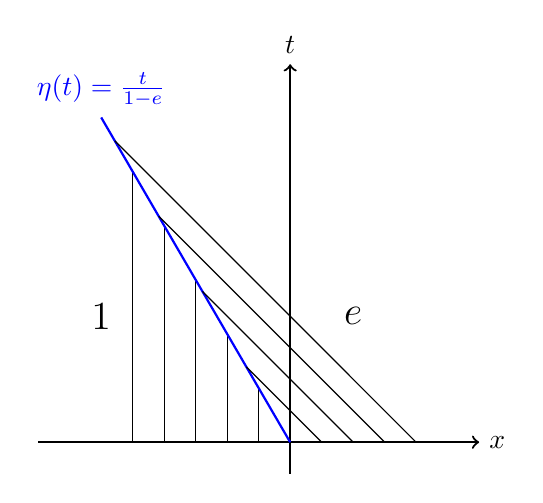
\begin{tikzpicture}[scale=0.8]

                  % Draw axes
                  \draw[thick, ->] (-4,0) -- (3,0) node[right] {$x$};
                  \draw[thick, ->] (0,-0.5) -- (0,6) node[above] {$t$};

                  % Vertical lines when x_0 < 0
                  \draw (-2.5,0) -- (-2.5,2.5/0.582);
                  \draw (-2,0) -- (-2,2/0.582);
                  \draw (-1.5,0) -- (-1.5,1.5/0.582);
                  \draw (-1,0) -- (-1,1/0.582);
                  \draw (-0.5,0) -- (-0.5,0.5/0.582);

                  % Function η(t) = t/(1-e) ≈ t/(-1.718) ≈ -0.582t
                  % Draw this as a function of x (treating x as t)
                  \draw[thick, blue] (0,0) -- (-3,3/0.582) node[above] {$\eta(t) = \frac{t}{1-e}$};

                  % Line x = -t + 1 when x_0 > 0, rearranged as t = -x + x_0
                  % Extended to meet the blue line
                  \pgfmathdeclarefunction{f}{1}{%
                      \pgfmathparse{#1/(1-0.582)}
                  }
                  \draw (0.5,0) -- ({(-0.582)*f(0.5)}, {f(0.5)});
                  \draw (1,0) -- ({(-0.582)*f(1)}, {f(1)});
                  \draw (1.5,0) -- ({(-0.582)*f(1.5)}, {f(1.5)});
                  \draw (2,0) -- ({(-0.582)*f(2)}, {f(2)});

                  % Add region labels
                  % Region to the left of the blue line (where solution = 1)
                  \node at (-3, 2) {\Large $1$};

                  % Region to the right of the blue line (where solution = e)
                  \node at (1, 2) {\Large $e$};
              \end{tikzpicture}
          \end{center}
          In the end, the only weak solution, i.e. the only solution the does satisfy the jump condition,
          to this problem is
          \[
              u(x,t) = \begin{cases}
                  1  & x < \eta(t) \\
                  e, & x > \eta(t)
              \end{cases}
          \]
          Now it's easy to check that the entropy condition is not satisfied, since for
          any \(E>0\) and \(a > 0\) we can find a couple of points \(x\) and \(t\) such
          that
          \[
              \underbrace{u(x+a,t)}_{=e} - \underbrace{u(x,t)}_{=1} > \frac{Ea}{t}.
          \]
          The idea is just to take \((x, t)\) such that \(x + a > \eta(t)\) and \(x <
          \eta(t)\) and \(t\) big enough to make sure that $e-1>Ea/t$.
\end{itemize}

\newpage
\begin{exercise}
    Let \(\Omega \subset \real^3\) be a bounded Lipschitz domain. Prove that the problem
    \begin{equation*}
        \begin{cases}
            \grad \cdot u = 0, & \text{in } \Omega,          \\
            u  = 0,            & \text{on } \partial \Omega,
        \end{cases}
    \end{equation*}
    has infinitely many solutions in \(C^\infty(\Omega) \cap C^0(\overline{\Omega})\).
\end{exercise}
We can prove this with the help of Helmoltz decomposition. We can write any vector field \(u\) as the sum of a solenoidal and an irrotational part
\[
    u = \grad \phi + \grad \times \psi.
\]
where \(\phi\) is the scalar potential and \(\psi\) is the vector potential.
Our constraint is that the divergence of \(u\) is zero, so we have
\[
    \grad \cdot u = \grad \cdot \grad \phi + \grad \cdot \grad \times \psi = \Delta \phi = 0 \quad \Rightarrow \quad \grad \phi = \text{const.}
\]
This means that the scalar potential is constant and we can rewrite the
decomposition
\[
    u = \grad \phi + \grad \times \psi = \grad \times \psi + C
\]
Now, choosing \(\psi\) such that satisfies the boundary condition, we can have
infinitely many solutions, since
\[
    \grad \cdot u = \grad \cdot \grad \times \psi + \grad \cdot C = 0 \quad \forall \psi \in  C^\infty(\Omega) \cap C^0(\overline{\Omega}).
\]

\newpage
\begin{exercise}
    Let \(\Omega \subset \real^n\) be a smooth bounded open set. Prove that the problem
    \begin{equation*}
        \begin{cases}
            \Delta u = u^3, & \text{in } \Omega,          \\
            u = 0,          & \text{on } \partial \Omega,
        \end{cases}
    \end{equation*}
    admits a unique classical solution and determine it.
\end{exercise}
We can prove the uniqueness of the solution by using the energy method. We multiply the equation by \(u\) and integrate over \(\Omega\)
\[
    \int_\Omega u \Delta u \, dx = \int_\Omega u^4 \, dx.
\]
Using the divergence theorem we have
\[
    -\int_\Omega \abs{\grad u}^2 \, dx = \int_\Omega u^4 \, dx.
\]
We have that the left side is negative, while the right side is positive, so
the only way to have a solution is to have \(u = 0\). This is the unique
solution to the problem.

\newpage
\subsection{July 2023}
\begin{exercise}
    Consider the two second order sobolev spaces \(H^2_0(-1, 1)\) and \(H^2(-1, 1) \cap H^1_0(-1, 1)\).
    \begin{enumerate}
        \item Prove that the map
              \[
                  (u, v) \longmapsto \int_{-1}^1 \left[ u''(x) v''(x) + u'(x) v'(x) + u(x) v(x) \right] \, dx
              \]
              defines a scalar product that turns both Sobolev spaces into Hilbert spaces.
        \item Prove that the map
              \[
                  (u, v) \longmapsto \int_{-1}^1 u''(x) v''(x) \, dx
                  \tag{(M)}
              \]
              defines a scalar product that turns both Sobolev spaces into Hilbert spaces.
        \item Determine a basis of the orthogonal complement of \(H^2_0(-1, 1)\) into
              \(H^2(-1, 1)\cap H^1_0(-1, 1)\) with respect to the scalar product \((M)\).
    \end{enumerate}
\end{exercise}
We start by checking the properties of the scalar product
\begin{remark}
    Let \(X\) be a vector space and we define a function
    \[
        \begin{aligned}
            \langle \cdot, \cdot \rangle : X \times X & \longrightarrow \real            \\
            (u, v)                                    & \longmapsto \langle u, v \rangle
        \end{aligned}
    \]
    such that for all \(u, v, w \in X\) and \(\alpha \in \real\) we have
    \begin{enumerate}
        \item \(\langle u, u \rangle \leq 0\), and \(\langle u, u \rangle = 0 \iff u = 0\) (non-degeneracy),
        \item \(\langle u, v \rangle = \langle v, u \rangle\) (symmetry),
        \item \(\langle \alpha u + \beta v, w \rangle = \alpha \langle u, w \rangle + \beta \langle v, w \rangle\) (linearity),
    \end{enumerate}
    then \(\langle \cdot, \cdot \rangle\) is a scalar product.
\end{remark}
Now we check if the given scalar products satisfy the properties.
\begin{enumerate}
    \item Starting with the first one
          \[
              \begin{aligned}
                  \langle u, u \rangle & = \int_{-1}^1 \left[ u''(x)^2 + u'(x)^2 + u(x)^2 \right] \, dx \geq 0, \\
                  \langle u, u \rangle & = 0 \iff u''(x) = u'(x) = u(x) = 0 \quad \forall x \in (-1, 1).
              \end{aligned}
          \]
          is true because in the first case is the sum of squares, and in the second case
          we have that \(u = 0\) means that all its derivatives are zero.

          For the symmetry property we see that is defined as sum of products, so it is
          symmetric.

          Then we check the linearity
          \[
              \begin{aligned}
                  \langle \alpha u + \beta v, w \rangle & = \int_{-1}^1 \left[ (\alpha u + \beta v)''(x) w''(x) + (\alpha u + \beta v)'(x) w'(x) + (\alpha u + \beta v)(x) w(x) \right] \, dx \\
                                                        & = \alpha \int_{-1}^1 \left[ u''(x) w''(x) + u'(x) w'(x) + u(x) w(x) \right] \, dx +                                                 \\
                                                        & + \beta \int_{-1}^1 \left[ v''(x) w''(x) + v'(x) w'(x) + v(x) w(x) \right] \, dx                                                    \\
                                                        & = \alpha \langle u, w \rangle + \beta \langle v, w \rangle.
              \end{aligned}
          \]
          This is true because derivatives and integrals are linear operators, and we can
          say that this map defines a scalar product. Now we need to check that the
          induced norm is complete, meaning that each Cauchy sequence converges. We have
          the norm
          \[
              \norm{u}_* = \sqrt{\langle u, u \rangle} = \sqrt{\int_{-1}^1 \left[ u''(x)^2 + u'(x)^2 + u(x)^2 \right] \, dx}.
          \]
          The standard norm in \(H^2_0(-1, 1)\) is
          \[
              \norm{u}_{H^2_0} = \sqrt{\int_{-1}^1 u''(x)^2 \, dx}.
          \]
          We can see that the two norms are equivalent, starting with the inequality
          \begin{align*}
              \norm{u}_{H^2_0} & \leq \norm{u}_*
          \end{align*}
          we only need to prove the opposite inequality. We start from \(\int_{-1}^1 -u''(x) u (x) \, dx \) and obtain
          \[
              \begin{split}
                  \frac{1}{2} \norm{u''(x)}^2_{L^2} + \frac{1}{2} \norm{u}^2_{L^2} = \int_{-1}^1 \frac{u''(x)^2}{2} + \frac{u(x)^2}{2} \, dx \geq \int_{-1}^1 u''(x) u(x) \, dx = \\= \int_{-1}^1 u'(x) u'(x) \, dx - \cancel{\left. u'(x) u(x) \right|_{-1}^1} = \norm{u'}^2_{L^2}.
              \end{split}
          \]
          Since by Poincaré inequality we have that \(\norm{u}_{L^2} \leq C
          \norm{u''}_{L^2}\), we have that \(\norm{u'}_{L^2}^2 \leq C
          \norm{u''}_{L^2}^2\), and also \(\norm{u}_{L^2}^2 \leq C \norm{u''}_{L^2}^2\).
          This means
          \[
              \norm{u}_{L^2}^2 + \norm{u'}_{L^2}^2 + \norm{u''}_{L^2}^2 \leq C \norm{u''}_{L^2}^2 \quad \Rightarrow \quad \norm{u}_* \leq C \norm{u}_{H^2_0}.
          \]
          This means that the two norms are equivalent, and since \(H^2_0(-1, 1)\) is
          complete, also the space defined by the scalar product is complete.

          Now we do the same proof for the space \(H^2(-1, 1) \cap H^1_0(-1, 1)\). We
          have the norm
          \[
              \norm{u}_* = \sqrt{\int_{-1}^1 \left[ u''(x)^2 + u'(x)^2 + u(x)^2 \right] \, dx}.
          \]
          The standard norm in \(H^2(-1, 1) \cap H^1_0(-1, 1)\) is
          \[
              \norm{u}_{H^2} = \sqrt{\int_{-1}^1 u''(x)^2 + u'(x)^2 \, dx}.
          \]
          We can clearly see that
          \[
              \norm{u}_{H^2} \leq \norm{u}_* \leq C \norm{u}_{H^2}.
          \]
          Now let's prove the othe inequality. by Poincaré inequality we have that
          \(\norm{u}_{L^2} \leq C \norm{u''}_{L^2}\), so we have the same reasoning as
          before.
    \item For the second scalar product we have
          \[
              \begin{aligned}
                  \langle u, u \rangle & = \int_{-1}^1 u''(x)^2 \, dx \geq 0,             \\
                  \langle u, u \rangle & = 0 \iff u''(x) = 0 \quad \forall x \in (-1, 1).
              \end{aligned}
          \]
          Same reasoning as before, also for the symmetry and linearity properties, so
          also this map defines a scalar product. Now we need to check that the induced
          norm is complete, meaning that each Cauchy sequence converges. For the first
          space \(H^2_0(-1, 1)\) we have the norm is already the standard norm, so the
          space is complete. For the second space \(H^2(-1, 1) \cap H^1_0(-1, 1)\) we
          have the norm
          \[
              \norm{u}_* = \sqrt{\int_{-1}^1 u''(x)^2 \, dx}.
          \]
          complies with the inequality
          \[
              \norm{u}_* \leq \norm{u}_{H^2\cap H^1_0}.
          \]
          To check the opposite inequality we start from \(\int_{-1}^1 -u''(x) u (x) \,
          dx \) and obtain
          \[
              \begin{split}
                  \frac{1}{2} \norm{u''(x)}^2_{L^2} + \frac{1}{2} \norm{u}^2_{L^2} = \int_{-1}^1 \frac{u''(x)^2}{2} + \frac{u(x)^2}{2} \, dx \geq \int_{-1}^1 u''(x) u(x) \, dx = \\= \int_{-1}^1 u'(x) u'(x) \, dx - \cancel{\left. u'(x) u(x) \right|_{-1}^1} = \norm{u'}^2_{L^2}.
              \end{split}
          \]
          So we have that \(\norm{u''}_{L^2}^2 \geq \norm{u'}_{L^2}^2\). Since
          \[
              \norm{u}_{H^2}^2 = \norm{u''}_{L^2}^2 + \norm{u'}_{L^2}^2 \leq C \norm{u''}_{L^2}^2 = C \norm{u}_*^2
          \]

    \item We now need to determine a basis of the orthogonal complement of \(H^2_0(-1,
          1)\) into \(H^2(-1, 1)\cap H^1_0(-1, 1)\) with respect to the scalar product
          \((M)\). To do so, we need to find all the functions \(v \in H^2_0(-1, 1)\)
          such that
          \[
              \int_{-1}^1 u''(x) v''(x) \, dx = 0 \quad \forall u \in H^2(-1, 1)\cap H^1_0(-1, 1).
          \]
          Integrating by parts we have
          \[
              \int_{-1}^1 u''(x) v''(x) \, dx = \cancel{\left. v'(x) u''(x) \right|_{-1}^1} - \int_{-1}^1 u'''(x) v'(x) \, dx = 0.
          \]
          Again integrating by parts we have
          \[
              -\int_{-1}^1 u'''(x) v'(x) \, dx = -\cancel{\left. v(x) u'''(x) \right|_{-1}^1} + \int_{-1}^1 u''''(x) v(x) \, dx = 0.
          \]
          So we have obtained
          \[
              \int_{-1}^1 u''''(x) v(x) \, dx = 0 \quad \forall u \in H^2(-1, 1)\cap H^1_0(-1, 1).
          \]
          Which is the weak formulation of the problem
          \[
              \begin{cases}
                  u''''(x) = 0, & \text{in } (-1, 1),          \\
                  u = 0         & \text{on } \partial (-1, 1).
              \end{cases}
          \]
          The general solution of this problem is
          \[
              u(x) = a + bx + cx^2 + d x^3.
          \]
          Since we have the boundary condition \(u(1) = u(-1) = 0\) we have that
          \[
              \begin{cases}
                  a + b + c + d = 0, \\
                  a - b + c - d = 0.
              \end{cases}
          \]
          Solving this gives us \(b = -d\) and \(a = -c\), so the general solution is
          \[
              u(x) = c(x^2 - 1) + d(x^3 - x).
          \]
          and the basis of the orthogonal complement is given by
          \[
              \left\{ x^2 - 1, x^3 - x \right\}.
          \]
\end{enumerate}

\newpage
\begin{exercise}
    Write the weak formulation of the forced stationary Navier-Stokes equations under Dirichlet boundary conditions in a smooth bounded domain \(\Omega \subset \real^n\) and explain why the assumption \(n \leq 4\) is needed.
\end{exercise}
We start by writing the stationary Navier-Stokes equations
\[
    \begin{cases}
        - \eta \Delta u + \left( u \cdot \grad \right) u + \grad p = f & \Omega         \\
        \div u = 0                                                     & \Omega         \\
        u = 0                                                          & \partial\Omega
    \end{cases}
\]
where \(\Omega \subset \real^n\), \(\partial\Omega \in C^1\), and \(n \leq 4\).
\begin{remark}
    About the term \(\left( u \cdot \grad \right) u\), we have that (\(n = 3\))
    \[
        u = \begin{pmatrix}
            u_1 \\
            u_2 \\
            u_3
        \end{pmatrix} \quad \text{and} \quad \grad = \begin{pmatrix}
            \partial_1 \\
            \partial_2 \\
            \partial_3
        \end{pmatrix}
    \]
    So combining the two we have
    \[
        \begin{split}
            \left( u \cdot \grad \right) u = \begin{pmatrix}
                                                 u_1 \partial_1 + u_2 \partial_2 + u_3 \partial_3
                                             \end{pmatrix} \begin{pmatrix}
                                                               u_1 \\
                                                               u_2 \\
                                                               u_3
                                                           \end{pmatrix} = \begin{pmatrix}
                                                                               u_1 \partial_1 u_1 + u_2 \partial_2 u_1 + u_3 \partial_3 u_1 \\
                                                                               u_1 \partial_1 u_2 + u_2 \partial_2
                                                                               u_2 + u_3 \partial_3 u_2                                     \\
                                                                               u_1 \partial_1 u_3 + u_2 \partial_2 u_3 + u_3 \partial_3 u_3
                                                                           \end{pmatrix}
        \end{split}
    \]
    which is the so-called convective term.
\end{remark}
As functional spaces we choose the spaces introduced in the previous exercise about the Stokes problem \(\bm{V}, \bm{G_1}, \bm{G_2}, \bm{G_3}\).
\begin{remark}
    \(\bm{V} \coloneqq \left\{ f \in \bm{H}^1_0(\Omega) \mid \grad \cdot f = 0 \right\}\) is the space of divergence-free functions.
    We also introduce three spaces:
    \begin{itemize}
        \item \(\bm{G}_1 \coloneqq \left\{ f \in \bm{L}^2(\Omega) \mid \grad \cdot f = 0, \gamma_\nu f = 0 \right\}\)
        \item \(\bm{G}_2 \coloneqq \left\{ f \in \bm{L}^2(\Omega) \mid \grad \cdot f = 0, \exists g \in H^1(\Omega) \text{ s.t. } f = \grad g \right\}\)
        \item \(\bm{G}_3 \coloneqq \left\{ f \in \bm{L}^2(\Omega) \mid \exists g \in H^1_0(\Omega) \text{ s.t. } f = \grad g \right\}\)
    \end{itemize}
\end{remark}
We now multiply the equation by a test function \(v \in \bm{V}\) and obtain
\[
    \begin{split}
        - \eta \int_\Omega \Delta u v \, dx + \int_\Omega \left( u \cdot \grad \right) u v \, dx + \int_\Omega \grad p \cdot v \, dx = \int_\Omega f v \, dx
    \end{split}
\]
We integrate by parts the first term and obtain
\[
    \begin{split}
        \eta \int_\Omega \grad u : \grad v \, dx + \int_\Omega \left( u \cdot \grad \right) u \cdot v \, dx + \underbrace{\int_\Omega \grad p \cdot v \, dx}_{=0} = \int_\Omega f v \, dx
    \end{split}
\]
The term \(\int_\Omega \grad p v \, dx\) is zero because \(v \in \bm{V}
\subseteq \bm{G_1}\) and \(\grad p \in \bm{G_2} \oplus \bm{G_3} =
\bm{G_1}^\perp\). We can now write the weak formulation of the problem
\[
    \begin{split}
        \text{Find } u \in \bm{V} \text{ such that } \eta \int_\Omega \grad u : \grad v \, dx + \int_\Omega \left( u \cdot \grad \right) u \cdot v \, dx = \langle f, v \rangle \qquad \forall v \in \bm{V}
    \end{split}
\]
Now we need to explain why the assumption \(n \leq 4\) is necessary. We need to
understand in which space the convective term lies and that \(v \in \bm{V}
\Rightarrow \grad v \in \bm{L}^2(\Omega)\).
\begin{itemize}
    \item[\(n = 2\)] In the bidimensional case, we have that \(u \in \bm{V} \Rightarrow u \in \bm{L}^p(\Omega) \, \forall 1 \leq p < \infty\). Since \(u \cdot \grad u\) is a product of a function in \(\bm{L}^p(\Omega)\) and a function in \(\bm{L}^2(\Omega)\), we have that \(u \cdot \grad u \in \bm{L}^2(\Omega) \, \forall q < 2\).
          \[
              \begin{pmatrix*}
                  \bm{H}^1_0(\Omega) \subset \bm{L}^p{(\Omega)} & \forall 1 \leq p < \infty \\
                  \bm{L}^{p'}(\Omega) \subset \bm{H}^{-1}(\Omega) & \forall 1 < p \leq \infty
              \end{pmatrix*}
              \Rightarrow u \cdot \grad u \in \bm{H}^{-1}(\Omega)
          \]
    \item[\(n = 3\)] In the tridimensional case, Sobolev embedding gives us \(u \in \bm{V} \Rightarrow u \in \bm{L}^6(\Omega)\). In this case we have that \(u \cdot \grad u \in \bm{L}^{3/2}(\Omega)\), because we have that \(u \in \bm{L}^6(\Omega)\) and \(\grad u \in \bm{L}^2(\Omega)\), and by Holder's inequality \(\frac{1}{6} + \frac{1}{2} + \frac{1}{r} = 1 \Rightarrow r = 3\) and the dual of \(\bm{L}^{3}(\Omega)\) is \(\bm{L}^{3/2}(\Omega)\).
          \[
              \begin{pmatrix*}
                  \bm{H}^1_0(\Omega) \subset \bm{L}^6{(\Omega)}  \\
                  \bm{L}^{6/5}(\Omega) \subset \bm{H}^{-1}(\Omega)
              \end{pmatrix*}
              \Rightarrow u \cdot \grad u \in \bm{L}^{3/2}(\Omega) \subset \bm{L}^{6/5}(\Omega) \subset \bm{H}^{-1}(\Omega)
          \]
    \item[\(n = 4\)] In the four-dimensional case, we have that \(u \in \bm{V} \Rightarrow u \in \bm{L}^4(\Omega)\). In this case we have that \(u \cdot \grad u \in \bm{L}^{4/3}(\Omega)\), because we have that \(u \in \bm{L}^4(\Omega)\) and \(\grad u \in \bm{L}^2(\Omega)\), and by Holder's inequality \(\frac{1}{4} + \frac{1}{2} + \frac{1}{r} = 1 \Rightarrow r = 4\) and the dual of \(\bm{L}^{4}(\Omega)\) is \(\bm{L}^{4/3}(\Omega)\).
          \[
              \begin{pmatrix*}
                  \bm{H}^1_0(\Omega) \subset \bm{L}^4{(\Omega)}  \\
                  \bm{L}^{4/3}(\Omega) \subset \bm{H}^{-1}(\Omega)
              \end{pmatrix*}
              \Rightarrow u \cdot \grad u \in \bm{H}^{-1}(\Omega)
          \]
    \item[\(n = 5\)] In the five-dimensional case, we have that \(u \in \bm{V} \Rightarrow u \in \bm{L}^{10/3}(\Omega)\). In this case we have that \(u \cdot \grad u \in \bm{L}^{5/4}(\Omega)\), because we have that \(u \in \bm{L}^{10/3}(\Omega)\) and \(\grad u \in \bm{L}^2(\Omega)\), and by Holder's inequality \(\frac{3}{10} + \frac{1}{2} + \frac{1}{r} = 1 \Rightarrow r = 5\) and the dual of \(\bm{L}^{5}(\Omega)\) is \(\bm{L}^{5/4}(\Omega)\).
          \[
              \begin{pmatrix*}
                  \bm{H}^1_0(\Omega) \subset \bm{L}^{10/3}{(\Omega)}  \\
                  \bm{L}^{10/7}(\Omega) \subset \bm{H}^{-1}(\Omega)
              \end{pmatrix*}
              \nRightarrow u \cdot \grad u \in \bm{L}^{10/7}(\Omega) \subset \bm{H}^{-1}(\Omega) \text{ because } \frac{5}{4} < \frac{10}{7}
          \]
          Because \(L^q \subset L^p\) if \(p < q\), in \(n = 5\) we do not have that \(u
          \cdot \grad u \in \bm{H}^{-1}(\Omega)\).
\end{itemize}

\newpage
\begin{exercise}
    It is known that if \(w(\cdot, t) \in \mathcal{S}(\real)\) satisfies \(w_t + 6(w - \epsilon w^2)w_x + w_{xxx} = 0\) in \(\real \times \real^+\), then, for all \(\epsilon \geq 0\),
    the function \(u \coloneqq w + \epsilon w_x - \epsilon^2 w^2\) satisfies the Korteweg-de Vries equation
    \[
        u_t + 6uu_x + u_{xxx} = 0 \quad \text{in } \real \times \real^+.
    \]
    Prove that the Korteweg-de Vries equation has infinitely many conserved
    quantities.
\end{exercise}
We will add the assumptions that we know that mass and momentum, and energy are conserved for the KdV equation.
To prove this, we start by rewriting the equation in \(w\) as
\[
    w_t + \left(3w^2 - 2\epsilon^2 w^3\right)_x + \left(w_{xx}\right)_x = 0 \Rightarrow u \text{ solves KdV } \Rightarrow \int w \text{ is conserved for all } \epsilon \geq 0.
\]
Then we write \(w = w(x, t; \epsilon)\) to highlight the dependence on
\(\epsilon\). It can be proved that this dependence \(\epsilon \mapsto w(x, t;
\epsilon)\) is analytic, so we can write
\[
    w(x, t; \epsilon) = \sum_{n=0}^\infty \epsilon^n w_n(x, t).
\]
which is the power series expansion of \(w\) in \(\epsilon\), and \(
\frac{d}{dt} \int w_n \, dx = 0 \text{ because mass is conserved.} \) At this
point we rewrite \(u\) as
\begin{align*}
    u & = w + \epsilon w_x - \epsilon^2 w^2 =                                                                                                            \\
      & = \sum_{n=0}^\infty \epsilon^n w_n + \sum_{n=0}^\infty \epsilon^{n+1} (w_{n})_x - \sum_{n=0}^\infty \epsilon^{n+2} w_n^2 =                       \\
      & = w_0 + \epsilon \left[w_1 + (w_0)_x\right] + \epsilon^2 \left[w_2 + (w_1)_x - w_0^2\right] + \epsilon^3 \left[w_3 + (w_2)_x - 2w_0 w_1\right] + \\
      & + \epsilon^4 \left[w_4 + (w_3)_x - 2w_0 w_2 - w_1^2\right] + R_4(\epsilon).
\end{align*}
Where in the last step we used the MacLaurin expansion in term of \(\epsilon\). But \(u\) has no dependence on \(\epsilon\), so we have that \((\cdot)\epsilon^n = 0\) for all \(n\).
\begin{align*}
     & w_0 = u,                                                                    \\
     & w_1 + (w_0)_x = -(w_0)_x = -u_x,                                            \\
     & w_2 + (w_1)_x - w_0^2 = u^2 - u_{xx},                                       \\
     & w_3 + (w_2)_x - 2w_0 w_1 = -u_{xxx} - 4uu_x,                                \\
     & w_4 + (w_3)_x - 2w_0 w_2 - w_1^2 = 5 u_x^2 + 6 u u_{xx} + u_{xxxx} + 2 u^3.
\end{align*}
Now we integrate all the equations in \(x\) and we obtain
\begin{align*}
    \int w_0 \, dx & = \int u \, dx = 0, \text{ mass}                                                                               \\
    \int w_1 \, dx & = -\underbrace{\int u_x \, dx}_{\text{\tiny div. form}} = 0, \text{ conserved}                                 \\
    \int w_2 \, dx & = \int u^2 \, dx - \int u_{xx} \, dx = \int u^2 \, dx, \text{ momentum}                                        \\
    \int w_3 \, dx & = -\int u_{xxx} \, dx - 4 \int u u_x \, dx = - \int \left(2 u^2 + u_{xx}\right)_x \, dx = 0, \text{ conserved} \\
    \int w_4 \, dx & = 5 \int u_x^2 \, dx + 6 \int u u_{xx} \, dx + \int u_{xxxx} \, dx + 2 \int u^3 \, dx =                        \\
                   & \underset{\mathclap{\text{IPP}}}{=} \int \left(2 u^3 - u_x^2\right) \, dx = 0, \text{ energy}.
\end{align*}
We find infinitely many conserved quantities for the KdV equation, with an increasing power of \(u\).

\newpage
\subsection{September 2023}
\begin{exercise}
    Let \(\Omega \subset \real^2\) be a bounded open set of class \(C^1\), and let \(f \in L^2(\Omega)\). Consider the Dirichlet problem
    \begin{equation*}
        \begin{cases}
            u_{tt} - \left(\partial_x^2 u + 2 \partial_y^2 u - 2 \partial_{xy} u\right) = f, & \text{in } \Omega \times (0, T),          \\
            u = 0,                                                                           & \text{on } \partial \Omega \times (0, T), \\
            u(x,0) = u_0(x),                                                                 & x \in \Omega,                             \\
            u_t(x,0) = u_1(x),                                                               & x \in \Omega.
        \end{cases}
        \tag{(P)}
    \end{equation*}
    \begin{enumerate}
        \item For a suitable symmetric matrix \(A\), write the PDE appearing in (P) in the
              form \(u_{tt} - \div(A \grad u) = f\).
        \item Write the weak formulation of (P).
        \item Sketch the proof of existence and uniqueness of a solution of (P), explaining
              to which functional spaces is expected to belong.
    \end{enumerate}
\end{exercise}
\begin{enumerate}
    \item We start by writing the PDE in the form \(u_{tt} - \div(A \grad u) = f\). We
          have that
          \[
              u_{tt} - \left(A_{11} u_{xx} + A_{22} u_{yy} + 2A_{12} u_{xy}\right) = f.
          \]
          We can write the matrix \(A\) as
          \[
              A = \begin{pmatrix}
                  2  & -1 \\
                  -1 & 2
              \end{pmatrix}
          \]
          and the PDE becomes
          \[
              u_{tt} - \div (A \grad u) = f.
          \]
    \item To write the weak formulation of the problem we first recall the space of
          weakly continuous functions
          \begin{remark}
              Let \(H\) be a Hilbert space. The space of weakly continuous functions over \([0, T]\) is defined as
              \[
                  \begin{split}
                      C_w^0([0, T]; H) = \left\{ u \in L^\infty(0, T; H) \mid \lim_{t \to t_0} (u(t) - u(t_0), v)_H = 0, \quad \forall t_0 \in [0, T], \forall v \in H \right\}
                  \end{split}
              \]
          \end{remark}
          Then choose an adequate Hilbert triplet, keeping in mind that this problem is equipped with Dirichlet boundary conditions. We can choose the Hilbert triplet
          \[
              V = H^1_0(\Omega) \subset H = L^2(\Omega) \subset V' = H^{-1}(\Omega).
          \]
          The weak formulation of the problem is then obtained by multiplying the
          equation by a test function \(v \in V\) and integrating over \(\Omega\)
          \begin{align*}
              \int_\Omega f(t) v \, dx & = \int_\Omega u_{tt} v \, dx + \int_\Omega \div(A \grad u)v \, dx =                                                                                  \\
                                       & = \int_\Omega u_{tt} v \, dx - \cancel{\int_{\partial\Omega} \partial_\nu u v \, d\sigma} + \int_\Omega \left[A \grad u \cdot \grad v\right] \, dx = \\
                                       & = \int_\Omega u_{tt} v \, dx + \int_\Omega \underbrace{A \grad u \cdot \grad v}_{B(u, v)} \, dx
          \end{align*}
          The weak formulation of the problem is then
          \[
              \begin{split}
                  \text{Find } u(t) \in C^0([0, T]; H) \cap C_w^0([0, T]; V) \text{ such that } \\
                  u' \in C_w^0([0, T]; H), u'' \in L^2(0, T; V') \text{ and }                   \\
                  \begin{cases}
                      \langle u_{tt}(t), v \rangle + B(u(t), v) = (f(t), v)_H \\
                      u(0) = u_0, \quad u'(0) = u_1
                  \end{cases}\quad \forall v \in V, \text{ in } \mathcal{D}(0, T).
              \end{split}
          \]
    \item To sketch the proof of existence and uniqueness of a solution of the problem we
          need to use the Galerkin method. The advantage of the Galerkin method is that
          is finite-dimensional, so we can have as much regularity as we want. Let
          \(\left\{V_m\right\}\) be a Galerkin sequence for \(V\), and therefore for
          \(H\). Then, \(\exists \left\{u_0^m\right\} \subset V_m\) and \(\exists
          \left\{u_1^m\right\} \subset V_m\) such that \(u_0^m \to u_0\) in \(V\) and
          \(u_1^m \to u_1\) in \(H\). Let \(m = \dim V_m\) and consider a basis
          \(\left\{w_k^m\right\}\) for \(V_m\) orthonormal in \(H\). We now look for
          \(u_m = u_m(t)\) such that
          \[
              u_m(t) = \sum_{k=1}^m g_k^m(t) w_k^m
          \]
          Moreover, for \(1 \leq k \leq m\) we have the system
          \[
              \begin{cases}
                  g_m''(t) + B_m g_m(t) = \gamma_m(t) \\
                  g_m(0) = g_0^m, \quad g_m'(0) = g_1^m
              \end{cases}
          \]
          Since \(g_m(t)\) is the unique solution of the system, we have that \(g_m(t)\)
          uniquely determines \(u_m(t)\). Then it is possible, starting from
          \[
              \frac{1}{2}\frac{d}{dt} \left[\norm{u_m'(t)}_H^2 + \norm{u_m(t)}_V^2\right] = \left(f(t), u_m(t)\right)_H \qquad \text{a.e in } [0, T],
              \tag*{(E)}
          \]
          to obtain the following a priori estimates
          \[
              \norm{u_0}_{L^\infty(0, T; V)} \leq C_1 \qquad \norm{u_1}_{L^\infty(0, T; H)} \leq C_2
          \]
          And it can be shown that the weak formulation can be recovered up to a
          subsequence, and that \(u\) admits a weak derivative \(u' \in L^\infty(0, T;
          H)\), and also that \(u'' \in L^2(0, T; V')\). Since
          \[
              \begin{cases}
                  u \in L^\infty(0, T; V)  \\
                  u' \in L^\infty(0, T; H) \\
              \end{cases}
              \Rightarrow u \in C^0([0, T]; H)
          \]
          and \(V \subset H\), we have that \(u \in C^0([0, T]; H) \cap C_w^0([0, T];
          V)\) and we have existence, by proving the same result for \(u'\). Then we take
          two solutions \(u_1\) and \(u_2\) and we have that \(w = u_1 - u_2\) . Putting
          \(w\) in (E) we obtain
          \[
              \begin{cases}
                  \frac{1}{2}\frac{d}{dt} \left[\norm{w'(t)}_H^2 + \norm{w(t)}_V^2\right] = 0 \\
                  w(0) = 0, \quad w'(0) = 0
              \end{cases}
              \Rightarrow w = 0 \Rightarrow u_1 = u_2
          \]
          and we have uniqueness.
\end{enumerate}

\newpage
\begin{exercise}
    Consider the Burgers' equation
    \[
        u_t + u u_x = 0 \quad \text{in } \real \times \real^+.
    \]
    By the method of characteristics, find the solution with initial condition
    \[
        u(x,0) = \begin{cases}
            1,      & x < 0,     \\
            2 - 2x, & 0 < x < 1, \\
            0,      & x > 1.
        \end{cases}
    \]
    and determine whether it satisfies the entropy condition.
\end{exercise}
We start by writing the characteristics equations
\[
    \frac{du}{ds} = \frac{dt}{ds} \frac{du}{dt} + \frac{dx}{ds} \frac{du}{dx} = 0
\]
we have that \(u\) is constant along the characteristics and \(t=s\) since the
initial condition is given at \(t=0\). Now we find the characteristics
equations from
\[
    x(t) = x_0 + u(x_0, t) t
\]
which gives us
\[
    x(t) = \begin{cases}
        x_0 + t,           & x_0 < 0,     \\
        x_0 + (2 - 2x_0)t, & 0 < x_0 < 1, \\
        x_0,               & x_0 > 1.
    \end{cases}
\]
Drawing the characteristics we have
\begin{center}
    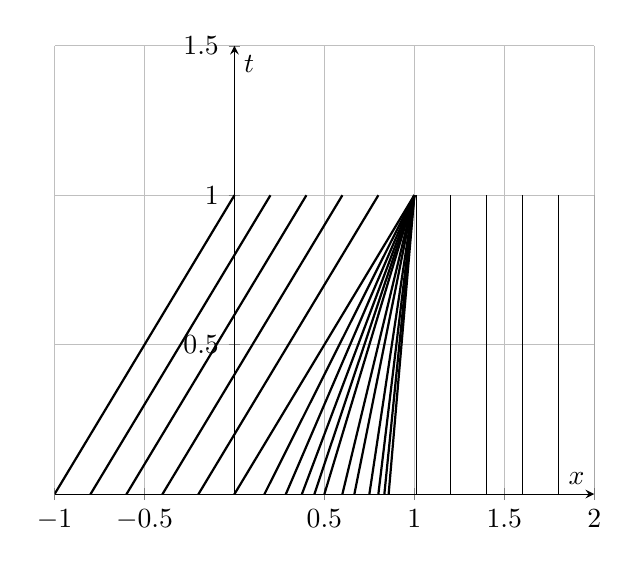
\begin{tikzpicture}
        \begin{axis}[
                xlabel={$x$}, ylabel={$t$},
                xmin=-1, xmax=2, ymin=0, ymax=1.5,
                axis lines=middle, grid=major,
                samples=20, domain=-2:1, legend pos=outer north east
            ]

            % Plot characteristics for u_0(x) = 1 for x <= 0

            \addplot[black, thick, domain=-2:-0.6] {x -0.4}; % Characteristic with slope 1
            \addplot[black, thick, domain=-2:-0.8] {x - 0.2}; % Characteristic with slope 1
            \addplot[black, thick, domain=-1:1] {x}; % Characteristic with slope 1
            \addplot[black, thick, domain=-1:0.8] {x + 0.2}; % Characteristic with slope 1
            \addplot[black, thick, domain=-1:0.6] {x + 0.4}; % Characteristic with slope 1
            \addplot[black, thick, domain=-1:0.4] {x + 0.6}; % Characteristic with slope 1
            \addplot[black, thick, domain=-1:0.2] {x + 0.8}; % Characteristic with slope 1
            \addplot[black, thick, domain=-1:0] {x + 1}; % Characteristic with slope 1

            % Plot characteristics for u_0(x) = 2 - 2x for 0 < x < 1
            \addplot[black, thick,domain=0:1] {x - (2 - 2*x) * 0.1};
            \addplot[black, thick,domain=0:1] {x - (2 - 2*x) * 0.2};
            \addplot[black, thick,domain=0:1] {x - (2 - 2*x) * 0.3};
            \addplot[black, thick,domain=0:1] {x - (2 - 2*x) * 0.4};
            \addplot[black, thick,domain=0:1] {x - (2 - 2*x) * 0.5};
            \addplot[black, thick,domain=0:1] {x - (2 - 2*x) * 0.75};
            \addplot[black, thick,domain=0:1] {x - (2 - 2*x)};
            \addplot[black, thick,domain=0:1] {x - (2 - 2*x) * 1.5};
            \addplot[black, thick,domain=0:1] {x - (2 - 2*x) * 2};
            \addplot[black, thick,domain=0:1] {x - (2 - 2*x) * 2.5};
            \addplot[black, thick,domain=0:1] {x - (2 - 2*x) *3};

            % Plot characteristics for u_0(x) = 0 for x > 1
            \draw[color=black]
            (axis cs:1.01, 0) -- (axis cs:1.01, 1);
            \draw[color=black]
            (axis cs:1.2, 0) -- (axis cs:1.2, 1);
            \draw[color=black]
            (axis cs:1.4, 0) -- (axis cs:1.4, 1);
            \draw[color=black]
            (axis cs:1.6, 0) -- (axis cs:1.6, 1);
            \draw[color=black]
            (axis cs:1.8, 0) -- (axis cs:1.8, 1);
            \draw[color=black]
            (axis cs:2, 0) -- (axis cs:2, 1);
        \end{axis}
    \end{tikzpicture}
\end{center}
that the characteristic do not intersect at least until \(t=1\).
Therefore, the function \(u(x,t)\) is defined continuous in \(\real \times [0, 1)\) and it is written as
\[
    u(x,t) = \begin{cases}
        1,                 & x \leq t,  \\
        \frac{2-2x}{1-2t}, & t < x < 1, \\
        0,                 & x \geq 1.
    \end{cases}
\]
We want to extend the solution to \(t > 1\). We need the solution to undergo a
jump, so given \(x = \eta(t)\) the curve of discontinuity, we have that
\[
    u(x, t) = \begin{cases}
        u_- = 1, & x < \eta(t) \\
        u_+ = 0, & x > \eta(t)
    \end{cases}
\]
The jump conditions states that
\[
    \eta'(t) \cdot \left[u_+ - u_-\right] = \left[B(u_+) - B(u_-)\right] \quad \text{on } \Gamma
\]
Here we have that \(B(u) = \frac{u^2}{2}\), so the jump condition becomes
\[
    \eta'(t) = \frac{u_+^2 - u_-^2}{u_+ - u_-} = \frac{1}{2}
\]
and the solution is
\[
    \eta(t) = \frac{t}{2} + C
\]
But, we know that \(\eta(1) = 1\), so \(C = 1/2\) and the solution is
\[
    u(x,t) = \begin{cases}
        1, & x < \frac{1}{2}(t+1), \\
        0, & x > \frac{1}{2}(t+1).
    \end{cases}
\]
Which is a discontinuous solution.

To satisfy the entropy condition we need to have that the characteristics on
both sides of the shock point towards the shock. To ensure this the condition
\(s = \eta'(t)\) should be less than the speed of the characteristic on the
right side and greater than the speed of the characteristic on the left side.
We have
\begin{align*}
    \text{Left side:}  & \quad u_-(x,t) = 1, \Rightarrow \frac{1}{2} < 1, \quad \text{True} \\
    \text{Right side:} & \quad u_+(x,t) = 0, \Rightarrow \frac{1}{2} > 0, \quad \text{True}
\end{align*}
Therefore the solution satisfies the entropy condition.

\newpage
\begin{exercise}
    Let \(\Omega \subset \real^n\) \(n \geq 2\) be a bounded open domain with \(\partial\Omega \in C^\infty\) and consider the boundary value problem
    \[
        \begin{cases}
            -\Delta u = f & \Omega         \\
            u = 0         & \partial\Omega
        \end{cases}
        \tag*{(P)}
    \]
    \begin{enumerate}
        \item Assuming that \(f \in H^{-1}(\Omega)\), write the weak formulation of (P).
        \item Prove that this problem admits a unique weak solution.
        \item Show that the unique solution \(u\) satisfies the Dirichlet principle.
        \item If \(f \in L^2(\Omega)\), in which space dimension \(n\) is it guaranteed that
              the solution \(u\) belongs to \(C^0(\overline{\Omega})\)?
    \end{enumerate}
\end{exercise}
\begin{enumerate}
    \item We start by writing the weak formulation of the problem. First we define a
          suitable function space, in this case we have \(V \in H^1_0(\Omega)\). We
          multiply the equation by a test function \(v \in V\) and obtain
          \[
              \begin{split}
                  -\int_\Omega \Delta u v \, dx = \int_\Omega f v \, dx \qquad \forall v \in V
              \end{split}
          \]
          We integrate by parts the left-hand side and obtain
          \[
              \begin{split}
                  \int_\Omega \grad u \grad v \, dx = \underbrace{\langle f, v \rangle}_{\text{bc } f \in H^{-1}} \qquad \forall v \in V
              \end{split}
          \]
          Then we obtain the weak formulation of the problem
          \[
              \begin{split}
                  \text{Find } u \in H^1_0(\Omega) \text{ such that } \int_\Omega \grad u \grad v \, dx =  \langle f, v \rangle \qquad \forall v \in V
              \end{split}
          \]
    \item Then we state the Dirichlet principle for the homogeneous Dirichlet problem
          \begin{remark}
              Let \(\Omega \subset \real^n\) be a bounded and Lipschitz domain and let \(f \in H^{-1}(\Omega), \alpha \geq 0\). Then the problem (P) admits a unique solution \(u \in V\) such that
              \[
                  \int_\Omega \grad u \grad v \, dx = \langle f, v \rangle \qquad \forall v \in V
              \]
              Moreover, \(u\) is the unique minimizer of the functional
              \[
                  J(u) = \frac{1}{2} \int_\Omega \abs{\grad u}^2 \, dx - \langle f, u \rangle
              \]
          \end{remark}
          A sketch of the proof goes as follows. We start by defining the functional
          \begin{align*}
              a: V \times V & \longrightarrow \real                         \\
              (u, v)        & \longmapsto \int_\Omega \grad u \grad v \, dx
          \end{align*}
          We have that \(a(u,v)\) is a continuous and coercive bilinear form. Then we can apply the Lax-Milgram theorem to obtain the existence of a unique solution \(u \in V\).

          To prove that the solution is the unique minimizer of the functional we need to
          observe that the functional \(J(u)\) is convex.
    \item Now we will prove that the unique solution \(u\) is the minimizer of the
          functional \(J(u)\). We start by recalling \(J(u)\)
          \[
              J(u) = \frac{1}{2} \int_\Omega \abs{\grad u}^2 \, dx - \langle f, u \rangle
          \]
          Assume \(\bar{u} \in V\) is a solution of the weak formulation of the problem.
          Then \(\exists w \in V\) such that \(u = \bar{u} + w\). We have that
          \[
              \begin{split}
                  J(u) = J(\bar{u} + w) = \frac{1}{2} \int_\Omega \abs{\grad \bar{u} + \grad w}^2 \, dx - \langle f, \bar{u} + w \rangle = \\
                  =J(\bar{u}) + \underbrace{\frac{1}{2}\int_\Omega \abs{\grad w}^2 \, dx}_{\geq 0} + \underbrace{\int_\Omega \grad \bar{u} \grad w \, dx - \langle f, w \rangle}_{\text{\tiny def. of weak solution } = 0} \geq J(\bar{u})
              \end{split}
          \]
          So, if \(w \neq 0\) we have that \(J(u) > J(\bar{u})\). Then, if \(\bar{u}\) is
          the weak solution, it is also the minimizer of the functional.
    \item To prove that the solution \(u\) belongs to \(C^0(\overline{\Omega})\) we need
          Sobolev embedding. We know that \(f \in H^m(\Omega)\) implies that \(u \in
          H^{m+2}(\Omega)\). We have that \(f \in L^2 \Rightarrow u \in H^2\) By Sobolev
          embedding, \(u \in C^0(\overline{\Omega})\) if \(n < 2s\), where \(s\) is the
          Sobolev exponent. Therefore, if \(n < 4\) we have that the solution \(u\)
          belongs to \(C^0(\overline{\Omega})\).
\end{enumerate}

\newpage
\subsection{January 2024}
\begin{exercise}
    For given constants \(\alpha, \beta, \gamma \in \real\), consider the Cauchy problem
    \[
        \begin{cases}
            u_{t} - \alpha u_{xx} - \beta u_{x}^4 + \gamma u^3u_x = 0, & (x,t) \in \real \times (0, \infty), \\
            u(x,0) = u_0(x),                                           & x \in \real,                        \\
        \end{cases}
        \tag*{(P)}
    \]
    \begin{enumerate}
        \item Find conditions on \(\alpha, \beta, \gamma\) ensuring mass conservation for
              regular solutions of (P).
        \item Find conditions on \(\alpha, \beta, \gamma\) ensuring momentum conservation for
              regular solutions of (P).
        \item When \(\beta = 0\), find a first-order ODE on \(g\) giving a necessary
              condition to have solitary wave solutions of (P).
    \end{enumerate}
\end{exercise}
\begin{enumerate}
    \item To have mass conservation we need \(\frac{\partial}{\partial t}\int_\real
          u(x,t) \, dx = 0\). We have that
          \[
              \begin{split}
                  \frac{\partial}{\partial t}\int_\real u(x,t) \, dx = \int_\real u_t(x,t) \, dx = \int_\real \left(- \alpha u_{xx} - \beta u_{x}^4 - \gamma u^3u_x\right) \, dx =
              \end{split}
          \]
          Let's see each term separately
          \[
              \begin{split}
                  \int_\real - \alpha u_{xx} \, dx = -\alpha \left.u_x\right|_\real = 0
              \end{split}
          \]
          This term goes to zero because we have that \(u \in \mathcal{S}(\real)\), so it
          is zero \(\forall \alpha\). The third term becomes
          \[
              \begin{split}
                  \int_\real - \gamma u^3u_x \, dx = -\frac{\gamma}{4} \left. u^4 \right|_\real = 0
              \end{split}
          \]
          same as before, this term goes to zero because we have that \(u \in
          \mathcal{S}(\real)\), so it is zero \(\forall \gamma\). The second term becomes
          \[
              \begin{split}
                  \int_\real - \beta u_{x}^4 \, dx = 0 \iff \beta = 0
              \end{split}
          \]
          Therefore, the condition for mass conservation is \(\beta = 0\).
    \item To have momentum conservation we need \(\frac{\partial}{\partial t}\int_\real
          u(x,t)^2 \, dx = 0\). We have that
          \[
              \begin{split}
                  \frac{\partial}{\partial t}\int_\real u(x,t)^2 \, dx = \int_\real 2u(x,t)u_t(x,t) \, dx = \int_\real 2u(x,t)\left(- \alpha u_{xx} - \beta u_{x}^4 - \gamma u^3u_x\right) \, dx
              \end{split}
          \]
          Let's see each term separately
          \[
              \begin{split}
                  -2\alpha \int_\real u u_{xx} \, dx = -\alpha \int_\real (u_x)^2 \, dx = 0 \iff \alpha = 0
              \end{split}
          \]
          The second term becomes
          \[
              \begin{split}
                  -2\beta \int_\real u u_{x}^4 \, dx = 0 \iff \beta = 0
              \end{split}
          \]
          The third term becomes
          \[
              \begin{split}
                  -2\gamma \int_\real u^4u_x \, dx = -\frac{\gamma}{5} \int_\real (u^5)_x \, dx = 0
              \end{split}
          \]
          Therefore, the condition for momentum conservation is \(\alpha = \beta = 0\).
    \item When \(\beta = 0\) we have that the equation becomes
          \[
              \begin{split}
                  u_{t} - \alpha u_{xx} + \gamma u^3u_x = 0
              \end{split}
          \]
          Solitary waves are solutions of the form \(u(x,t) = g(x + ct)\). We substitute
          this into the equation and obtain
          \[
              \begin{split}
                  cg'(x + ct) - \alpha g''(x + ct) + \gamma g(x + ct)^3g'(x + ct) = 0
              \end{split}
          \]
          We perform the change of variables \(s = x + ct\) and obtain
          \[
              \begin{split}
                  cg'(s) - \alpha g''(s) + \gamma g(s)^3g'(s) = 0
              \end{split}
          \]
          We can rewrite this as
          \[
              \begin{split}
                  \frac{d}{ds} \left[ cg(s) - \alpha g'(s) + \frac{\gamma}{4} g(s)^4 \right] = 0
              \end{split}
          \]
          Integrating this equation we obtain
          \[
              \begin{split}
                  cg(s) - \alpha g'(s) + \frac{\gamma}{4} g(s)^4 = C
              \end{split}
          \]
          where \(C\) is a constant. This is the first-order ODE that gives a necessary
          condition to have solitary wave solutions of the problem.
\end{enumerate}

\newpage
\begin{exercise}
    Let \(\Omega \subset \real^n (n \geq 2)\) be a bounded smooth domain, let \(a\) be a measurable function in \(\Omega\).
    Consider the problem
    \[
        \begin{cases}
            - \Delta u = a(x) u^3 & \Omega         \\
            u = 0                 & \partial\Omega
        \end{cases}
        \tag*{(P)}
    \]
    Under which assumptions on the space dimension n can we write a variational
    formulation of problem (P) in \(H^1_0(\Omega)\)?

    For each of these dimensions find the most general assumptions on \(a\) that
    allow to write the variational formulation.

    Finally, write the variational formulation.
\end{exercise}

First, a quick reminder on Sobolev embedding, which will be very useful a.e. in
this document
\begin{remark}
    Let \(\Omega \subseteq \real^n\) open with \(\partial\Omega \in \text{Lip}\), \(s \geq 0\),
    \[
        H^s(\Omega) \subset
        \begin{cases}
            L^p(\Omega) \qquad \forall \, 2 \leq p \leq 2^* & \text{if } n > 2s \\
            L^p(\Omega) \qquad \forall \, 2 \leq p < \infty & \text{if } n = 2s \\
            C^0(\bar{\Omega})                               & \text{if } n < 2s
        \end{cases}
    \]
    Increasing \(s\) increases the regularity, while increasing \(n\) decreases it.

    The exponent \(2^*\) is called critical exponent and is defined as \(2^*
    \coloneqq \frac{2n}{n - 2s}\).

    If \(\Omega\) is bounded, all these embeddings are compact except \(H^s(\Omega)
    \subset L^{2^*}\) when \(n > s\).
\end{remark}

Since we want to know the variational formulation in \(H^1_0\) we have \(s =
1\) and need to check \(n = 2, n \geq 3\). Remember a variational formulation
makes sense if \(\int_\Omega fv < \infty\).
\begin{itemize}
    \item[\(n = 2\).] In this case we have \(u, v \in H^1_0(\Omega)\), so by Sobolev embedding we know \(u, v \in L^p(\Omega)\) for \(2 \leq p < \infty\).
          \[
              \abs{\int_\Omega a(x) u^3 v}  \, dx \leq \int_\Omega \abs{a(x)} \abs{u^3} \abs{v} \, dx \underset{Holder}{\leq} \left(\int_\Omega \abs{a(x)}^r\right)^{\frac{1}{r}} \left(\int_\Omega \abs{u^3}^p \right)^{\frac{1}{p}} \left(\int_\Omega \abs{v}^q \right)^{\frac{1}{q}} < \infty.
          \]
          To use Holder inequality we need to find \(r, p, q\) such that \(\frac{1}{r} +
          \frac{1}{p} + \frac{1}{q} = 1\). We see that,
          \[
              \frac{1}{r} + \frac{1}{p} + \frac{1}{q} = 1 \iff a(x) \in L^r(\Omega) \qquad \text{with } r > 1
          \]
    \item[\(n \geq 3\).] In this case we have \(u, v \in H^1_0(\Omega)\), so by Sobolev embedding we know \(u, v \in L^p(\Omega)\) for \(2 \leq p \leq 2^*\).
          We proceed as before, using Holder inequality, but decide to use \(p = \frac{2^*}{3}\) and \(q = \frac{1}{2^*}.\)
          \[
              \abs{\int_\Omega a(x) u^3 v}  \, dx \leq \int_\Omega \abs{a(x)} \abs{u^3} \abs{v} \, dx \underset{\mathclap{Holder}}{\leq} \left(\int_\Omega \abs{a(x)}^r\right)^{\frac{1}{r}} \left(\int_\Omega \abs{u}^{2^*} \right)^{\frac{3}{2^*}} \left(\int_\Omega \abs{v}^{2^*} \right)^{\frac{1}{2^*}} < \infty.
          \]
          In this case Holder inequality gives us
          \[
              \frac{1}{r} + \frac{3}{2^*} + \frac{1}{2^*} = 1 \iff \frac{1}{r} = 1 - \frac{4}{2^*} \iff r = \frac{2^*}{2^* - 4}
          \]
          Substituting \(2^* = \frac{2n}{n - 2}\) we get \(r = \frac{n}{-n + 4}\). Since
          \(r > 0\) we need \(n < 4\). In this case we have \(a(x) \in L^3(\Omega)\) for
          \(n = 3\), but also \(a(x) \in L^\infty(\Omega)\) for \(n = 4\).
\end{itemize}

At this point we can write the weak formulation of the problem. We multiply the
equation by a test function \(v \in H^1_0(\Omega)\) and obtain
\[
    \int_\Omega - \Delta u v \, dx = \int_\Omega a(x) u^3 v \, dx \qquad \forall v \in H^1_0(\Omega)
\]
We integrate by parts the left-hand side and obtain
\[
    \int_\Omega \nabla u \nabla v \, dx = \int_\Omega a(x) u^3 v \, dx \qquad \forall v \in H^1_0(\Omega)
\]
This is the weak formulation of the problem. This is well posed if
\begin{table}[h]
    \centering
    \begin{tabular}{|c|c|}
        \hline
        Dimension  & Assumptions on $a(x)$        \\
        \hline
        $n = 2$    & $a \in L^r(\Omega)$, $r > 1$ \\
        $n = 3$    & $a \in L^3(\Omega)$          \\
        $n = 4$    & $a \in L^\infty(\Omega)$     \\
        $n \geq 5$ & No variational formulation   \\
        \hline
    \end{tabular}
\end{table}

\newpage
\begin{exercise}
    Let \(\Omega \subset \real^2\) be a bounded, simply connected, smooth domain and \(\eta > 0\). Consider the inhomogeneous Dirichlet boundary value problem for the unforced Navier-Stokes equations
    \[
        \begin{cases}
            -\eta \Delta u + (u \cdot \grad )u + \grad p = f & \Omega         \\
            \div u = 0                                       & \Omega         \\
            u = (1,1)                                        & \partial\Omega
        \end{cases}
        \tag*{(P)}
    \]
    \begin{enumerate}
        \item Find an explicit solenoidal extension of the boundary datum.
        \item Prove that (P) admits a unique solution \(u\) for any \(\eta > 0\).
    \end{enumerate}
\end{exercise}

\begin{enumerate}
    \item We start by finding an explicit solenoidal extension of the boundary datum. We
          have that the boundary datum is \(u = (1,1)\) on \(\partial\Omega\). We can
          extend this to the whole domain by defining
          \[
              \begin{split}
                  u(x) = (1,1) \qquad \forall x \in \Omega
              \end{split}
          \]
          This is a solenoidal extension of the boundary datum because \(\div u = 0\).
    \item We will now prove uniqueness thanks to the theorem
          \begin{remark}[Uniqueness stationary N-S]
              If \(\exists \gamma > 0\) such that \(\norm{f}_{\bm{V'}} < \gamma\), then the problem (P) admits a unique solution.
          \end{remark}
          For the proof we start with the weak formulation of the problem.
          \[
              \begin{split}
                  \eta \int_\Omega \grad u : \grad v \, dx + \int_\Omega (u \cdot \grad) u \cdot v \, dx = \langle f, v \rangle \qquad \forall v \in \bm{V}
              \end{split}
          \]
          and define trilinear form
          \[
              \begin{split}
                  b(u, v, w) = \int_\Omega (u \cdot \grad) v \cdot w \, dx
              \end{split}
          \]
          Now we take \(v = u\) and obtain the following a priori bound
          \[
              \begin{split}
                  \eta \norm{u}_{\bm{V}}^2 = \langle f, u \rangle - \underbrace{\cancel{b(u, u, u)}}_{=0} \leq \norm{f}_{\bm{V'}} \norm{u}_{\bm{V}}
              \end{split}
          \]
          Thanks to the Cauchy-Schwarz inequality. We have that
          \[
              \begin{split}
                  \norm{u}_{\bm{V}} \leq \frac{\norm{f}_{\bm{V'}}}{\eta}
              \end{split}
          \]
          Now assume the existence of two solutions \(u_1\) and \(u_2\):
          \begin{align*}
              \eta \int_\Omega \grad u_1 : \grad v \, dx + b(u_1, u_1, v) & = \langle f, v \rangle \qquad \forall v \in \bm{V} \\
              \eta \int_\Omega \grad u_2 : \grad v \, dx + b(u_2, u_2, v) & = \langle f, v \rangle \qquad \forall v \in \bm{V}
          \end{align*}
          Subtracting the two equations with \(w = u_1 - u_2\) we obtain
          \[
              \begin{split}
                  \eta \int_\Omega \grad w : \grad w \, dx + b(u_1, u_1, v) - b(u_2, u_2, v) = 0 \qquad \forall v \in \bm{V}
              \end{split}
          \]
          We see that
          \begin{align*}
              b(u_1, u_1, v) - b(u_2, u_2, v) & = b(u_1, u_1, v) - b(u_1, u_2, v) + b(u_1, u_2, v) - b(u_2, u_2, v) \\
                                              & = b(u_1, u_1 - u_2, v) + b(u_1 - u_2, u_2, v)                       \\
                                              & = b(u_1, w, v) + b(w, u_2, v)                                       \\
          \end{align*}
          We can now rewrite the equation as
          \[
              \begin{split}
                  \eta \int_\Omega \grad w : \grad v \, dx= -b(w, u_2, v) - b(u_1, w, v) \qquad \forall v \in \bm{V}
              \end{split}
          \]
          Choosing \(v = w\) we obtain \(\eta \norm{w}_{\bm{V}}^2 = -b(w, u_2, w) -
          \cancel{b(u_1, w, w)}\). We have that
          \[
              \begin{split}
                  \eta \norm{w}_{\bm{V}}^2 = -b(w, u_2, w) \leq C \norm{w}_{\bm{V}}^2 \norm{u_2}_{\bm{V}}
              \end{split}
          \]
          where \(C\) is a constant depending on the domain. Substituting the a priori
          bound we have that
          \[
              \begin{split}
                  \eta \norm{w}_{\bm{V}}^2 \leq C_\Omega \frac{\norm{f}_{\bm{V'}}}{\eta} \norm{w}_{\bm{V}}^2
              \end{split}
          \]
          We can see that if
          \[
              \begin{split}
                  C_\Omega \frac{\norm{f}_{\bm{V'}}}{\eta} < \eta \Rightarrow \norm{w}_{\bm{V}} = 0 \Rightarrow w = 0 \Rightarrow \gamma = \frac{\eta^2}{C_\Omega}
              \end{split}
          \]
          we have that the problem admits a unique solution.
\end{enumerate}

\newpage
\begin{exercise}
    Prove that there exists at most one smooth solution \(u\) for the beam equation
    \[
        \begin{cases}
            u_{tt} + u_{xxxx} = f                         & (x,t) \in (0,1) \times (0, T) \\
            u(0, t) = u(1, t) = u_x(0, t) = u_x(1, t) = 0 & t \in [0, T]                  \\
            u(x, 0) = g(x), u_t(x, 0) = h(x)              & x \in [0, 1]
        \end{cases}
        \tag*{(P)}
    \]
    where \(f \in C^1([0,1] \times [0, T])\), \(g, h \in C^1([0,1])\) are given
    functions.
\end{exercise}

We start by assuming that there are two solutions \(u_1\) and \(u_2\). We
define \(w = u_1 - u_2\). We have that \(w\) satisfies the homogeneous beam
equation
\[
    \begin{cases}
        w_{tt} + w_{xxxx} = 0                         & (x,t) \in (0,1) \times (0, T) \\
        w(0, t) = w(1, t) = w_x(0, t) = w_x(1, t) = 0 & t \in [0, T]                  \\
        w(x, 0) = 0, w_t(x, 0) = 0                    & x \in [0, 1]
    \end{cases}
\]
We multiply the equation by \(w_t\) and integrate over \(x\)
\[
    \begin{split}
        \int_0^1 w_t w_{tt} + w_t w_{xxxx} \, dx = 0
    \end{split}
\]
The first term becomes
\[
    \begin{split}
        \int_0^1 w_t w_{tt} \, dx = \frac{1}{2} \frac{\partial}{\partial t} \int_0^1 w_t^2 \, dx = \frac{1}{2} \frac{\partial}{\partial t} \norm{w_t}_{L^2}^2
    \end{split}
\]
The second term becomes
\[
    \begin{split}
        \int_0^1 w_t w_{xxxx} \, dx = \cancel{\left. w_t w_{xxx} \right|_0^1} - \int_0^1 w_{tx} w_{xxx} \, dx = - \int_0^1 w_{tx} w_{xxx} \, dx = \\
        = -\cancel{\left. w_{tx} w_{xx} \right|_0^1} + \int_0^1 w_{txx} w_{xx} \, dx = \int_0^1 w_{txx} w_{xx} \, dx
    \end{split}
\]
which can be rewritten as
\[
    \begin{split}
        \int_0^1 w_{txx} w_{xx} \, dx = \frac{1}{2} \frac{\partial}{\partial t} \int_0^1 w_{xx}^2 \, dx = \frac{1}{2} \frac{\partial}{\partial t} \norm{w_{xx}}_{L^2}^2
    \end{split}
\]
Therefore we have that
\[
    \begin{split}
        \frac{1}{2} \frac{\partial}{\partial t} \left(\norm{w_t}_{L^2}^2 + \norm{w_{xx}}_{L^2}^2\right) = 0
    \end{split}
\]
which implies that
\[
    \begin{split}
        \norm{w_t}_{L^2}^2 + \norm{w_{xx}}_{L^2}^2 = \text{ constant} = F(t)
    \end{split}
\]
We have that \(F(t) = \text{ const.}\) and
\[
    \begin{split}
        F(0) = \norm{w_t(x, 0)}_{L^2}^2 + \norm{w_{xx}(x, 0)}_{L^2}^2 = 0
    \end{split}
\]
Since \(w_t(x, 0) = 0\) and \(w(x,0) = 0 \Rightarrow w_{xx}(x, 0) = 0\).
Therefore \(F(0) = 0\). We have that \(F(t) = 0\) for all \(t \in [0, T]\).
This implies that \(w_t = 0\) and \(w_{xx} = 0\). Therefore \(w = 0\) and the
solution is unique.

\newpage
\subsection{February 2024}
\begin{exercise}
    Let \(\Omega \subset \real^2\) be a bounded open set of class \(C^1\), and let \(f \in L^2(\Omega)\). Consider the Dirichlet problem
    \begin{equation*}
        \begin{cases}
            u_{t} - \left(\partial_x^2 u +  \partial_y^2 u - 2 \partial_{xy} u\right) = f, & \text{in } \Omega \times (0, T),          \\
            u = 0,                                                                         & \text{on } \partial \Omega \times (0, T), \\
            u(x,0) = u_0(x),                                                               & x \in \Omega,                             \\
        \end{cases}
        \tag{(P)}
    \end{equation*}
    \begin{enumerate}
        \item For a suitable symmetric matrix \(A\), write the PDE appearing in (P) in the
              form \(u_{tt} - \div(A \grad u) = f\).
        \item Write the weak formulation of (P).
        \item Sketch the proof of existence and uniqueness of a solution of (P), explaining
              to which functional spaces is expected to belong.
    \end{enumerate}
\end{exercise}
\begin{enumerate}
    \item We start by writing the PDE in the form \(u_{tt} - \div(A \grad u) = f\). We
          have that
          \[
              u_{t} - \left(A_{11} u_{xx} + A_{22} u_{yy} + 2A_{12} u_{xy}\right) = f.
          \]
          We can write the matrix \(A\) as
          \[
              A = \begin{pmatrix}
                  2 & 1 \\
                  1 & 1
              \end{pmatrix}
          \]
          and the PDE becomes
          \[
              u_{t} - \div (A \grad u) = f.
          \]
    \item To write the weak formulation we choose an adequate Hilbert triplet, keeping in
          mind that this problem is equipped with Dirichlet boundary conditions. We can
          choose the Hilbert triplet
          \[
              V = H^1_0(\Omega) \subset H = L^2(\Omega) \subset V' = H^{-1}(\Omega).
          \]
          The weak formulation of the problem is then obtained by multiplying the
          equation by a test function \(v \in V\) and integrating over \(\Omega\)
          \begin{align*}
              \int_\Omega f(t) v \, dx & = \int_\Omega u_{t} v \, dx + \int_\Omega \div(A \grad u)v \, dx =                                                                                  \\
                                       & = \int_\Omega u_{t} v \, dx - \cancel{\int_{\partial\Omega} \partial_\nu u v \, d\sigma} + \int_\Omega \left[A \grad u \cdot \grad v\right] \, dx = \\
                                       & = \int_\Omega u_{t} v \, dx + \int_\Omega \underbrace{A \grad u \cdot \grad v}_{B(u, v)} \, dx
          \end{align*}
          The weak formulation of the problem is then
          \[
              \begin{split}
                  \text{Find } u(t) \in L^2([0, T]; V)\cap C^0([0, T]; H)\text{ such that } \\
                  u' \in L^2([0, T];H)\text{ and }                                          \\
                  \begin{cases}
                      \langle u_{t}(t), v \rangle + B(u(t), v) = (f(t), v)_H \\
                      u(0) = u_0,
                  \end{cases}\quad \forall v \in V, \text{ in } \mathcal{D}(0, T).
              \end{split}
          \]
    \item To sketch the proof of existence and uniqueness of a solution of the problem we
          need to use the Galerkin method. The advantage of the Galerkin method is that
          is finite-dimensional, so we can have as much regularity as we want. Let
          \(\left\{V_m\right\}\) be a Galerkin sequence for \(V\), with a basis
          \(\left\{w_m \right\}\). We can now write the weak formulation of the problem
          in the Galerkin space
          \[
              \begin{split}
                  \text{Find } u_m \in H^1((0, T); V_m) \text{ such that } \\
                  \begin{cases}
                      \left(u_m'(t), v_m\right)_H + B(u_m(t), v_m) = \langle f(t), v_m \rangle_H  \quad \forall v_m \in V_m \\
                      u_m(0) = P_m u_0
                  \end{cases}
              \end{split}
          \]
          We now have a finite number of linear ODEs, and for \(1 \leq k \leq m\) we have
          \[
              u_m(t) = \sum_{k=1}^m g_k^m(t) w_k^m
          \]
          So we want to solve the following system
          \[
              \begin{cases}
                  g_m'(t) + B_m g_m(t) = \gamma_m(t) \\
                  g_m(0) = g_0^m,
              \end{cases}
          \]
          Since \(g_m(t)\) is the unique solution of the system, we have that \(g_m(t)\)
          uniquely determines \(u_m(t)\). Then it is possible, taking \(v_m = u_m\) to
          obtain
          \[
              \frac{1}{2}\frac{d}{dt}\norm{u_m(t)}_H^2 + B(u_m(t), u_m(t)) = \langle f(t), u_m(t) \rangle \quad \forall t \in (0, T)
              \tag*{(E)}
          \]
          Integrating and using some inequalities gives us two a priori bounds
          \[
              \norm{u_m(t)}_{L^\infty(0, T; H)} \leq K_1 \quad \text{and} \quad \norm{u_m(t)}_{L^2(0, T; V)} \leq K_2
          \]
          Since the bounds are in \(L^2(0, T; V)\) and \(L^\infty(0, T; H)\), we have
          that up to a subsequence
          \begin{align*}
              \int_0^T \left(u_m(t), v(t)\right)_H \, dt & \to \int_0^T \left(u(t), v(t)\right)_H \, dt \quad \forall v \in L^1(0, T; H) \\
              \int_0^T \left(u_m(t), v(t)\right)_V \, dt & \to \int_0^T \left(u(t), v(t)\right)_V \, dt \quad \forall v \in L^2(0, T; V)
          \end{align*}
          With these converges we are able to manage \(B(u_m, v_m)\) and \(\langle f, v_m \rangle\). We need some bounds on \(\langle u_t, v \rangle\). Using the weak derivative definition we can ``free'' the time derivative and obtain
          \[
              \begin{split}
                  - \int_0^T \left(u_m(t), v_t(t)\right)_H \phi'(t) \, dt - \left(u_m(0), v(0)\right)_H \phi(0) \\\to -\int_0^T \left(u(t), v_t(t)\right)_H \phi'(t) \, dt - \left(u(0), v(0)\right)_H \phi(0)
              \end{split}
          \]
          We can integrate by parts and obtain
          \[
              \begin{split}
                  -\int_0^T \left(u(t), v\right)_H \phi'(t) \, dt + \left(u(0), v(0)\right)_H \phi(0) = \int_0^T \langle u_t(t), v \rangle \phi(t) \, dt
              \end{split}
          \]
          We have then that
          \[
              \begin{split}
                  \langle u_t(t), v \rangle = - B(u(t), v) + \langle f(t), v \rangle
              \end{split}
          \]
          Since \(B(u,v)\) is a bilinear continuous and coercive form, if we fix \(v\) we
          have that \(B(u, v)\) is a linear continuous functional. Then we have
          \[
              \begin{split}
                  \langle u_t(t), v \rangle = \langle \mathcal{L}(t), v \rangle
              \end{split}
          \]
          with \(\mathcal{L}(t) = -B(u(t), v) + \langle f(t), v \rangle \in L^2(0, T;
          V')\). Then
          \[
              \begin{cases}
                  u \in L^2(0, T; V)   \\
                  u' \in L^2(0, T; V') \\
              \end{cases}
              \Rightarrow u \in C^0([0, T]; H).
          \]
          Then we take two solutions \(u_1\) and \(u_2\) and we have that \(w = u_1 -
          u_2\) . Putting \(w\) in (E) we obtain
          \[
              \begin{cases}
                  \frac{1}{2} \frac{d}{dt} \norm{w(t)}_H^2 + B(w(t), w(t)) = 0 \\
                  w(0) = 0
              \end{cases}
          \]
          Since both \(\norm{w(t)}_H^2\) and \(B(w(t), w(t))\) are positive, we have that
          \(\frac{1}{2} \frac{d}{dt} \norm{w(t)}_H^2 \leq 0\). This implies that \(w =
          0\) and the solution is unique.
\end{enumerate}

\newpage
\begin{exercise}
    Consider the conservation law with two different initial conditions
    \begin{equation*}
        a)\,\begin{cases}
            u_t - u^3 u_x = 0,    & x \in \real, t > 0, \\
            u(x,0) = \sqrt[3]{x}, & x \in \real,
        \end{cases}
        \qquad
        b)\,\begin{cases}
            u_t - u^3 u_x = 0,    & x \in \real, t > 0, \\
            u(x,0) = -\sqrt[3]{x} & x \in \real.
        \end{cases}
    \end{equation*}
    Determine the maximal domain \(A\) of definition of the solution as continuous function: explain if they are also of class \(C^1(A)\) and satisfy the entropy condition.
\end{exercise}
\begin{enumerate}
    \item[\textbf{a)}] We look for solutions \(u(x, t) \in C^1(\real \times (0, \infty))\) that satisfy the conservation law and the initial condition.
          Its characteristics are given by
          \[
              \frac{du}{dt} = \frac{dt}{ds} \frac{du}{dt} + \frac{dx}{ds} \frac{du}{dx} = 0
          \]
          means that \(u\) is constant along the characteristics and then
          \[
              u(x,t) = u(x_0,0) = \sqrt[3]{x_0}
          \]
          with \(t=s\) since the initial condition is given at \(t=0\).
          \[
              \frac{dx}{ds} = u_0^3 \quad \Rightarrow \quad x(s) = x_0 + s u_0^3
          \]
          Since \(u_0^3 = (\sqrt[3]{x_0})^3 = x_0\), we have that \(x(s) = x_0 + s x_0 =
          x_0(1+s)\). We can then write the solution as
          \[
              x(s) = x_0 + s x_0 = x_0(1+s) \quad \Rightarrow \quad x_0 = \frac{x}{1+s}.
          \]
          The solution is then
          \[
              u(x,t) = \sqrt[3]{\frac{x}{1+t}}.
          \]
          This is a classical solution that remains smooth for all \(x \in \real\) and
          \(t > 0\), so the maximal domain of definition is \(A = \real \times (0,
          \infty)\). Let's compute the derivatives of \(u\)
          \begin{align*}
              u_x(x,t) & = \frac{1}{3} \frac{1}{\sqrt[2]{\frac{x}{1+t}}^2}         \\
              u_t(x,t) & = -\frac{1}{3(1+t)^2} \frac{1}{\sqrt[3]{\frac{x}{1+t}}^2}
          \end{align*}
          These are not continuous at \(x=0\), so the solution is not of class \(C^1(A)\). Since we do not have a discontinuity in our solution, the entropy condition is satisfied.
    \item[\textbf{b)}] Now we look at the second case.

          Its characteristics are given by
          \[
              \frac{du}{dt} = \frac{dt}{ds} \frac{du}{dt} + \frac{dx}{ds} \frac{du}{dx} = 0
          \]
          means that \(u\) is constant along the characteristics and then
          \[
              u(x,t) = u(x_0,0) = -\sqrt[3]{x_0}
          \]
          with \(t=s\) since the initial condition is given at \(t=0\).
          \[
              \frac{dx}{ds} = u_0^3 \quad \Rightarrow \quad x(s) = x_0 + s u_0^3
          \]
          Since \(u_0^3 = (-\sqrt[3]{x_0})^3 = -x_0\), we have that \(x(s) = x_0 - s x_0
          = x_0(1-s)\). We can then write the solution as
          \[
              x(s) = x_0 + s x_0 = x_0(1+s) \quad \Rightarrow \quad x_0 = \frac{x}{1-s}.
          \]
          The solution is then
          \[
              u(x,t) = \sqrt[3]{\frac{x}{1-t}}.
          \]
          We can immediately see that this solution present a discontinuity in \(t=1\) so
          the maximal domain of definition is \(A = \real \times (0, 1)\). Let's compute
          the derivatives of \(u\)
          \begin{align*}
              u_x(x,t) & = -\frac{1}{3} \frac{1}{\sqrt[2]{\frac{x}{1+t}}^2}       \\
              u_t(x,t) & = \frac{1}{3(1+t)^2} \frac{1}{\sqrt[3]{\frac{x}{1+t}}^2}
          \end{align*}
          These are not continuous at \(x=0\), so the solution is not of class \(C^1(A)\). No idea about the entropy condition.
\end{enumerate}

\newpage
\begin{exercise}
    Let \(\Omega \subset \real^n\) with \(n \geq 2\) be a bounded domain with \(\partial \Omega \in C^\infty\) and let \(f \in H^3(\Omega)\). Determine the space dimension \(n\) for which the we can conclude that
    \begin{enumerate}
        \item \(f \in L^4(\Omega)\).
        \item \(f \in C^0(\overline{\Omega})\).
        \item \(\gamma_0 f \in H^{5/2}(\Omega)\).
    \end{enumerate}
\end{exercise}
We start by recalling the Sobolev embeddings with \(2s = 6\)
\begin{align*}
    H^3(\Omega) & \subset C^0(\Omega)                                               &  & \text{ if } n < 6 \\
    H^3(\Omega) & \subset L^p(\Omega) \qquad \forall 2 \leq p < \infty              &  & \text{ if } n = 6 \\
    H^3(\Omega) & \subset L^p(\Omega) \qquad \forall 2 \leq p \leq \frac{2n}{n - 6} &  & \text{ if } n > 6
\end{align*}
Then we check the statements
\begin{enumerate}
    \item In this case we have that \(f \in L^4(\Omega)\) if \(n = 6\), but we need to
          check when \(n > 6\). We have that \(2^* = \frac{2n}{n - 6}\) and we need to
          check if \(4 \leq 2^*\). We have that \(4 \leq \frac{2n}{n - 6}\) if \(n \leq
          12\).
    \item In this case we need to check if \(f \in C^0(\overline{\Omega})\). We have that
          \(f \in C^0(\overline{\Omega})\) if \(n < 6\).
    \item In this case we have \(\gamma_j f \in H^{s-j-1/2}(\Omega)\) with \(j = 0\). We
          have that \(\gamma_0(f) \in H^{3 - 0 - 1/2}(\partial\Omega) =
          H^{5/2}(\partial\Omega)\), this is true for all dimensions \(n\).
\end{enumerate}

\newpage

\begin{exercise}
    Let \(\Omega \coloneqq B(0, 1) \subset \real^n\), and let
    \[
        f(x) \coloneqq \frac{\log(1+\abs{x}^\alpha)}{\abs{x}^2}, \quad \text{with } \alpha > 0
    \]
    Find the values of \(\alpha\) for which \(f \in H^1(\Omega)\).
\end{exercise}
To check that a function is in \(H^1(\Omega)\) we need that
\begin{remark}
    \[
        H^1(\Omega) = \left\{ f \in L^2(\Omega) \mid \grad f \in L^2(\Omega) \right\}
    \]
\end{remark}
\textit{First step.} We start by verifying when \(f \in L^2(\Omega)\), i.e. when \(\int_\Omega \abs{f(x)}^2 \, dx < \infty\).
\[
    \begin{split}
        \int_\Omega \abs{f(x)}^2 \, dx = \int_\Omega \abs{\frac{\log(1+\abs{x}^\alpha)}{\abs{x}^2}}^2 \, dx
    \end{split}
\]
Since our domain is a ball, we can use spherical coordinates to compute the
integral
\begin{align*}
    \int_\Omega \abs{\frac{\log(1+\abs{x}^\alpha)}{\abs{x}^2}}^2 \, dx = \omega_n \int_0^1 \abs{\frac{\log(1+\rho^\alpha)}{\rho^2}}^2  \rho^{n-1} \, d\rho
\end{align*}
where \(\omega_n\) is the surface measure of the unit sphere in \(\real^n\).
At this point, we know that $\log(1+\rho^\alpha) \sim \rho^\alpha$ as $\rho \to 0$, so we study the convergence of the following integral
\begin{equation*}
    \int_0^1 \frac{\rho^{2\alpha}}{\rho^4} \rho^{n-1} \, d\rho < \infty \iff - 2 \alpha - n + 5 < 1 \iff \alpha > \frac{4-n}{2}
\end{equation*}
So we have that \(f \in L^2(\Omega)\) if \(\alpha > \frac{4-n}{2}\).\\
\vspace{0.1cm}\\
\textit{Second step.} We now need to check when \(\grad f \in L^2(\Omega)\) and we proceed by computing the gradient of \(f\).
We recall that
\begin{remark}
    In general, if \(f\) is radial, the modulus of the a.e. gradient is given by the modulus of the derivative with respect to the radial coordinate.
    \begin{equation*}
        \frac{\partial f}{\partial x_j} = \frac{\partial f}{\partial \rho} \frac{\partial \rho}{\partial x_j} = \frac{\partial f}{\partial \rho} \frac{x_j}{\abs{x}}
        \implies \abs{\grad f} = \sqrt{\sum_j \left(\frac{\partial f}{\partial x_j}\right)^2} = \abs{\frac{\partial f}{\partial \rho}} \frac{\abs{x}}{\abs{x}} = \abs{\frac{\partial f}{\partial \rho}}
    \end{equation*}
\end{remark}
\begin{align*}
    \frac{\partial f}{\partial \rho} & = \frac{\alpha\rho^{\alpha}}{(1 + \rho^\alpha)\rho^3} - \frac{\log(1 + \rho^\alpha)2}{\rho^3}       \\
    \abs{\grad f}                    & = \abs{\frac{\alpha\rho^{\alpha}}{(1 + \rho^\alpha)\rho^3} - \frac{\log(1 + \rho^\alpha)2}{\rho^3}}
\end{align*}
And now we check when this function is in \(L^2(\Omega)\)
\begin{align*}
    \int_\Omega \abs{\grad f}^2 \, dx = \omega_n \int_0^1 \abs{\frac{\alpha\rho^{\alpha}}{(1 + \rho^\alpha)\rho^3} - \frac{\log(1 + \rho^\alpha)2}{\rho^3}}^2 \rho{n-1}\, d\rho \\
\end{align*}
At this point, we exploit that $\abs{\grad f} \sim (\alpha-2)\rho^{\alpha-3}$ as $\rho \to 0$ if $\alpha \neq 2$.
So we check when the following integral is finite
\begin{equation*}
    \int_0^1 \rho^{2(\alpha-3)}\rho^{n - 1} \, d\rho < \infty \iff -2\alpha + 6 - n + 1 < 1 \iff \alpha > \frac{6-n}{2}
\end{equation*}
In the case \(\alpha = 2\) we have that $\abs{\grad f} \sim \rho^{2\alpha-3}$ as $\rho \to 0$, so we check the convergence of the integral
\begin{equation*}
    \int_0^1 \rho^{2(2\alpha-3)} \rho^{n-1} \, d\rho < \infty \iff -4\alpha + 6 - n + 1 < 1 \iff 2 = \alpha > \frac{6-n}{4} \text{ (satisfied for every } n \text{)}
\end{equation*}
So we have that \(\grad f \in L^2(\Omega)\) if \(\alpha > \frac{6-n}{2}\).\\
\\
\vspace{0.1cm}\\
\textit{Third step.} In order to justify other procedure and conclude that $f \in H^1(\Omega)$,
it remains to verify whether the weak derivative of \(f\) exists and coincides with the a.e. derivative.
We have that the weak derivative of \(f\) exists if
\begin{equation}\label{eq:weak_derivative2}
    \int_\Omega f \partial_{x_i} \phi \, dx = - \int_\Omega \partial_{x_i} f \phi \, dx \qquad \forall \phi \in \mathcal{D}(\Omega)
\end{equation}
We now consider that $\partial_{x_i} f$ is a.e. one and we want to verify that it satisfies this condition.
The main idea is to cut off the singularity of \(f\) in the origin in the following way, defining the set
\[
    \Omega_\epsilon = B(0, 1) \setminus B(0, \epsilon) = B_1 \setminus B_\epsilon = \left\{ x \in \real^n \mid \epsilon < \abs{x} < 1 \right\}
\]
Since \(f \in C^1(\Omega_\epsilon)\) we can apply the divergence theorem and
obtain
\begin{equation}\label{eq:divergence2}
    \int_{\Omega_\epsilon} f \partial_{x_i} \phi \, dx = -\int_{\Omega_\epsilon} \partial_{x_i} f \phi \, dx - \int_{\partial\Omega_\epsilon} f \phi \nu_i \, d\sigma
\end{equation}
So what we want to show is that taking the limit as \(\epsilon \to 0\) in \eqref{eq:divergence2} we get \eqref{eq:weak_derivative2}.
To do so we need to check that the boundary term goes to zero, and the other two terms converge to the ones in \eqref{eq:weak_derivative2}. \\
We start with the first term
\[
    \begin{split}
        \int_{\Omega_\epsilon} f \partial_{x_i} \phi \, dx = \int_{B_1} f \partial_{x_i} \phi \chi_{\Omega_\epsilon} \, dx
    \end{split}
\]
We want to claim that
\[
    \begin{split}
        \lim_{\epsilon \to 0^+} \int_{\Omega_\epsilon} f \partial_{x_i} \phi \, dx = \int_{B_1} f \partial_{x_i} \phi \, dx
    \end{split}
\]
To do so we need to swap the limit and the integral. We see that
\begin{itemize}
    \item \(f \partial_{x_i} \phi \chi_{\Omega_\epsilon} \underset{\epsilon \to 0}{\longrightarrow} f \partial_{x_i} \phi\) a.e. in \(B_1\)
    \item \(\abs{f \partial_{x_i} \phi \chi_{\Omega_\epsilon}} \leq \underbrace{\abs{f}}_{L^p(B_1)} \underbrace{\abs{\partial_{x_i} \phi}}_{L^q(B_1)} \in L^1(B_1)\)
\end{itemize}
We can now apply the Dominated Convergence Theorem and obtain the desired result.
The same process can be applied to
\[
    \begin{split}
        \int_{\Omega_\epsilon} \partial_{x_i} f \phi \, dx = \int_{B_1} \partial_{x_i} f \phi \chi_{\Omega_\epsilon} \, dx
    \end{split}
\]
It is clear now clear why we need to check that the boundary term goes to zero.
In particular it is composed by the following two integrals.
\[
    \begin{split}
        \int_{\partial\Omega_\epsilon} f \phi \nu_i \, d\sigma = \cancel{\int_{\partial B_1} f \phi \nu_i \, d\sigma} + \int_{\partial B_\epsilon} f \phi \nu_i \, d\sigma
    \end{split}
\]
And we can neglet the first one since we know that $\phi = 0$ on $\partial
    B_1$. Moreover,
\[
    \begin{split}
        \abs{\int_{\partial B_\epsilon} f \phi \nu_i \, d\sigma} & \leq \int_{\partial B_\epsilon} \abs{f} \abs{\phi} \underbrace{\abs{\nu_i}}_{\leq 1} \, d\sigma \leq \max_{\partial B_\epsilon} \abs{\phi} \int_{\{ \abs{x} = \epsilon \}} \abs{f} \, d\sigma \\
                                                                 & = \max_{\partial B_\epsilon} \abs{\phi} \frac{\log(1+\epsilon^\alpha)}{\epsilon^2} \omega_n \epsilon^{n-1} = C \frac{\log(1+\epsilon^\alpha)}{\epsilon^2} \epsilon^{n-1}
    \end{split}
\]
We have that
\[
    \begin{split}
        \lim_{\epsilon \to 0^+} \frac{\log(1+\epsilon^\alpha)}{\epsilon^2} \epsilon^{n-1} = \lim_{\epsilon \to 0^+} \frac{\epsilon^\alpha}{\epsilon^2} \epsilon^{n-1} = 0 \iff \alpha - 2 + n - 1 >  0 \iff \alpha > 3 - n
    \end{split}
\]
Since we know that $3 - n < \frac{6-n}{4}$ for every \(n > 2\), it's guaranteed
that the limit goes to zero if \(\alpha > \frac{6-n}{2}\). So we have shown
that $f \in H^1(\Omega)$ if \(\alpha \in \left(\max\left\{0,
\frac{6-n}{2}\right\}, \infty\right)\).\\


\section{Exams 2024/25}
\subsection{June 2024}
\begin{exercise}
    Let \(\Omega \subset \real^2\) be a bounded open set of class \(C^\infty\), let \(f \in \left[H^1(\Omega)\right]'\), \(g \in H^{1/2}(\partial \Omega)\), \(\alpha \in \real\) and \(A = (a_{ij})_{i, j=1,2}\) be a symmetric matrix. Write the weak formulation of the inhomogeneous Dirichlet problem
    \[
        \begin{cases}
            -\div(A \grad u) + \alpha u = f & \text{in } \Omega, \\
            u = g & \text{on } \partial \Omega.
        \end{cases}
    \]
    Then find sufficient conditions on \(A\) and \(\alpha\) such that this problem has a unique solution that can be identified through the Dirichlet principle.
    \end{exercise}
    The Dirichlet principle for the inhomogeneous Dirichlet problem states that 
    \begin{remark}
        Let \(\alpha > -\lambda_1\), where \(\lambda_1\) is the first eigenvalue of \(-\div(A \grad \cdot)\) with Dirichlet boundary conditions, \(f \in H^{-1}(\Omega)\) and \(g \in H^{1/2}(\partial \Omega)\). Then there exists a unique solution \(u \in K\) where \(K = \{u \in H^1(\Omega) : u-u_0 \in H^1_0(\Omega)\}\) and \(u_0 \in H^1(\Omega)\) is the function such that \(\gamma_0(u_0) = g\), for the weak formulation of the inhomogeneous Dirichlet problem
        \[
            \begin{split}
                \text{Find } u \in K \text{ such that } \int_\Omega A \grad u \cdot \grad v + \alpha u v \, dx = \langle f, v \rangle \text{ for all } v \in H^1_0(\Omega)
            \end{split}
        \]
    \end{remark}
    We first write the weak formulation of the inhomogeneous Dirichlet problem. Let \(u_0 \in H^1(\Omega)\) be the function such that \(\gamma_0(u_0) = g\). Then we define the space \(K = \{u \in H^1(\Omega) : u-u_0 \in H^1_0(\Omega)\}\). The weak formulation of the inhomogeneous Dirichlet problem is then
    \[
        \begin{split}
            \text{Find } u \in K \text{ such that } \int_\Omega A \grad u \cdot \grad v + \alpha u v \, dx = \langle f, v \rangle \text{ for all } v \in H^1_0(\Omega).
        \end{split}
    \]
    For \(\alpha\) to satisfy the Dirichlet principle, we need \(\alpha > -\lambda_1\).

    To find condition on \(A\), we need to check if the bilinear form \(a(u, v) = \int_\Omega A \grad u \cdot \grad v + \alpha u v \, dx\) is continuous and coercive. We have
    \[
        \begin{split}
            |a(u, v)| = \left|\int_\Omega A \grad u \cdot \grad v + \alpha u v \, dx\right| \leq \norm{A}_{L^\infty(\Omega)} \norm{\grad u}_{L^2(\Omega)} \norm{\grad v}_{L^2(\Omega)} + \abs{\alpha} \norm{u}_{L^2(\Omega)} \norm{v}_{L^2(\Omega)} \leq \\
            \leq C \norm{u}_{H^1(\Omega)} \norm{v}_{H^1(\Omega)}
        \end{split}
    \]
    We used the norm in \(L^\infty\) for \(A\) because we know that \(\grad u, \grad v \in L^2(\Omega)\) and by Holder's inequality we have
    \[
        \begin{split}
            \frac{1}{r} + \frac{1}{p} + \frac{1}{q} = 1 \Rightarrow \frac{1}{r} = 1 - \frac{1}{2} - \frac{1}{2} = 0 \Rightarrow r = \infty
        \end{split}
    \]
    So our first assumption is that \(A \in L^\infty(\Omega)\). We also need to check if the bilinear form is coercive, which means 
    \[
        \begin{split}
            a(u, u) \geq \norm{A} \norm{\grad u}_{L^2(\Omega)}^2 + \abs{\alpha} \norm{u}_{L^2(\Omega)}^2.
        \end{split}
    \]
    For this condition to hold true we choose two vectors \(\xi = \abs{\grad u} \in \real^2\) and we suppose that \(A\) is uniformly elliptic, i.e. there exists \(\lambda_0 > 0\) such that
    \[
        \begin{split}
            (A\xi, \xi) \geq \lambda_0 \abs{\xi}^2, \qquad \forall \xi \in \real^2.
        \end{split}
    \]
    This means we have a lower bound on the eigenvalues of \(A\). We can then write
    \[
        \begin{split}
            a(u, u) = \int_\Omega A \grad u \cdot \grad u + \alpha u^2 \, dx \geq \lambda_0 \norm{\grad u}_{L^2(\Omega)}^2 + \abs{\alpha} \norm{u}_{L^2(\Omega)}^2.
        \end{split}
    \]
    Summing up, we need 
    \begin{itemize}
        \item \(\alpha > -\lambda_1\),
        \item \(A \in L^\infty(\Omega)\),
        \item \(A\) is uniformly elliptic.
    \end{itemize}

\newpage
\begin{exercise}
    Let \(a \in \real, g \in C^2(\real)\) and consider the Cauchy problem
    \[
        \begin{cases}
            u_{t} + a u_{xx} + 2 u u_{x} = 0 & (x, t) \in \real \times (0, \infty), \\
            u(x, 0) = g(x) & x \in \real.
        \end{cases}
    \]
    \begin{enumerate}
        \item Prove the conservation of mass.
        \item In dependence of \(a\), discuss the conservation of momentum.
        \item Find solitary waves, if any.
    \end{enumerate}
\end{exercise}
\begin{enumerate}
    \item We first prove the conservation of mass. We have
    \[
        M(t) = \int_\real u(x, t) \, dx.
    \]
    In this case 
    \[
        \begin{split}
            \frac{d}{dt} M(t) = \frac{d}{dt} \int_\real u(x, t) \, dx = \int_\real u_t \, dx = -\int_\real (a u_{xx} + 2 u u_x) \, dx = \\ 
            = \underbrace{\int_\real -a(u_x)_x \, dx}_{\text{div. form} = 0} - \underbrace{\int_\real (u^2)_x}_{=0} \, dx = 0
        \end{split}
    \]
    \item We now discuss the conservation of momentum. We have
    \[
        \begin{split}
            \mathcal{M}(t) = \int_\real u(x, t) ^2 \, dx.
        \end{split}
    \]
    Its conservation is given by
    \[
        \begin{split}
            \frac{d}{dt} \mathcal{M}(t) = \frac{d}{dt} \int_\real u(x, t)^2 \, dx = \int_\real 2 u u_t \, dx 
        \end{split}
    \]
    We substitute the PDE into the integral
    \[
        \begin{split}
            \int_\real 2 u u_t \, dx = \int_\real 2 u (-a u_{xx} - 2 u u_x) \, dx = -2a \int_\real u u_{xx} \, dx - 4 \int_\real u^2 u_x \, dx = \\ 
            = \cancel{\left. -2a u u_x \right|_\real} + 2a \int_\real u_x^2 \, dx - \frac{4}{3} \underbrace{\int_\real (u^3)_x }_{=0} \, dx = 2a \int_\real u_x^2 \, dx
        \end{split}
    \]
    We have that momentum increases if \(a > 0\) and decreases if \(a < 0\). If \(a = 0\) then momentum is conserved.
    \item We now find solitary waves. We look for solutions of the form \(u(x, t) = g(x + ct)\). We substitute this into the PDE
    \[
        \begin{split}
            cg'(x + ct) + a g''(x + ct) + 2 g(x + ct) g'(x + ct) = 0
        \end{split}
    \]
    Performing the change of variables \(s = x + ct\) we get
    \[
        \begin{split}
            cg'(s) + a g''(s) + 2 g(s) g'(s) = 0
        \end{split}
    \]
    We can rewrite this as
    \[
        \begin{split}
            \frac{d}{ds} \left(cg(s) + a g'(s) + g(s)^2\right) = const.
        \end{split}
    \]
    We assume it is homogeneous, so we have
    \[
        \begin{split}
            g'(s) =- \frac{c}{a} g(s)  -\frac{1}{a} g(s)^2
        \end{split}
    \]
    This is a Bernoulli equation, which can be solved by the substitution \(y(s) = g(s)^{-1}\). We obtain
    \[
        y(s) = \frac{1}{g(s)} \Rightarrow y'(s) = -\frac{g'(s)}{g(s)^2} 
    \]
    We substitute this into the equation
    \[
        \begin{split}
            \left(\frac{c}{a} g(s)  + \frac{1}{a} g(s)^2\right) \frac{1}{g(s)^2} = \frac{c}{a} y(s) + \frac{1}{a} = y'(s)
        \end{split}
    \]
    So we have the ODE  
    \[
        \begin{split}
            y'(s) - \frac{c}{a} y(s) = \frac{1}{a}
        \end{split}
    \]
    We can solve this ODE by multiplying by the integrating factor \(e^{\int \frac{c}{a} \, ds}\)
    \[
        \begin{split}
            e^{\frac{c}{a}s} y'(s) - \frac{c}{a} e^{\frac{c}{a}s} y(s) = \frac{1}{a} e^{\frac{c}{a}s} \Rightarrow \left(e^{\frac{c}{a}s} y(s)\right)' = \frac{1}{a} e^{\frac{c}{a}s}
        \end{split}
    \]
    We can now integrate both sides
    \[
        \begin{split}
            e^{\frac{c}{a}s} y(s) = \frac{1}{a} \int e^{\frac{c}{a}s} \, ds \Rightarrow y(s) = \frac{1}{c} + C e^{-\frac{c}{a}s}
        \end{split}
    \]
    We can now substitute back \(y(s) = g(s)^{-1}\) and solve for \(g(s)\)
    \[
        \begin{split}
            g(s) = y(s)^{-1} = \frac{1}{\frac{1}{c} + C e^{-\frac{c}{a}s}}
        \end{split}
    \]
\end{enumerate}

\newpage

\begin{exercise}
    Prove that exists at most one smooth solution \(u\) for the telegraph equation
    \[
        \begin{cases}
            u_{tt} + d u_t - u_{xx} = f & (x, t) \in (0,1) \times (0, T), \\
            u(0, t) = u(1, t) = 0 & t \in (0, T), \\
            u(x, 0) = g(x), \quad u_t(x, 0) = h(x) & x \in (0, 1).
        \end{cases}
    \]
    Where \(d > 0\), \(g, h \in C^([0, 1])\) and \(f \in C([0, 1] \times [0, T])\).
\end{exercise}
We start by assuming that there are two solutions \(u_1\) and \(u_2\). We define \(v = u_1 - u_2\). We have the homogeneous problem
\[
    \begin{cases}
        v_{tt} + d v_t - v_{xx} = 0 & (x, t) \in (0,1) \times (0, T), \\
        v(0, t) = v(1, t) = 0 & t \in (0, T), \\
        v(x, 0) = 0, \quad v_t(x, 0) = 0 & x \in (0, 1).
    \end{cases}
\]
Now we use the energy method. We define the energy functional
\[
    \begin{split}
        E(t) = \frac{1}{2} \int_0^1 \left(v_t^2 + v_x^2\right) \, dx
    \end{split}
\]
Its derivative is 
\[
    \begin{split}
        \frac{d}{dt} E(t) = \int_0^t \left(v_t v_{tt} + v_x v_{xt}\right) \, dx = \int_0^1 v_t\left(-d v_t + v_{xx}\right) + \int_0^1 v_x v_{xt} \, dx = \\
        -\int_0^1 d v_t^2 + \cancel{\left. v_t v_x \right|_0^1} - \int_0^1 v_x v_{xt} \, dx  + \int_0^1 v_x v_{xt} \, dx = -d \int_0^1 v_t^2 \, dx \leq 0
    \end{split}
\]
We have that the energy is decreasing, but also that is always positive. Taking \(E(0)\) we have that \(E(0) = 0\). This means that \(E(t) = 0\) for all \(t\), which means that \(v = 0\) and therefore \(u_1 = u_2\).  
\newpage
\begin{exercise}
    Let \(\Omega \coloneqq B(0, 1) \subset \real^n\), and let 
    \[
        f(x) \coloneqq \frac{1}{\abs{x}^\alpha}, \quad \text{with } \alpha > 0
    \]
    Find the values of \(\alpha\) for which \(f \in H^2(\Omega)\).
\end{exercise}
To check that a function is in \(H^2(\Omega)\) we need recall its definition
\begin{remark}
\[H^2(\Omega) = \left\{ f \in L^2(\Omega) \mid D^\alpha f \in L^2(\Omega) \quad \forall \alpha : |\alpha|\leq 2\right\}\]
\end{remark}
and also the following fact
\begin{remark}
In $H^2 \cap H^1_0 (\Omega)$ the the following norms are equivalent
\begin{align*}
\norm{f}_{H^2(\Omega)}^2 &= \sum_{|\alpha| \leq 2} \norm{D^\alpha f}_{L^2(\Omega)}^2\\
\norm{f}^2_{*} &= \norm{\Delta f}_{L^2(\Omega)}^2 
\end{align*}
\end{remark}
So now we decide to exploit this fact studying the function $g=f-1$ and prove that it is in $H^2 \cap H^1_0(\Omega)$,
so that we can conclude immediately that \(f \in H^2(\Omega)\) as well.
From now on we will just write $f$ instead of $g$.\\
\vspace{0.1cm}\\
\textit{First step.}
We start by checking when \(f \in H^1(\Omega)\), i.e. when \(f \in L^2(\Omega)\) and \(\grad f \in L^2(\Omega)\). 
Thanks to the definition of \(f\) we automatically have that \(f \in H^1_0(\Omega)\) since it vanishes on the boundary of the ball.
We verify when \(f \in L^2(\Omega)\), i.e. \(\int_\Omega \abs{f(x)}^2 \, dx < \infty\).
\[
    \begin{split}
        \int_\Omega \abs{f(x)}^2 \, dx = \int_\Omega \abs{\frac{1}{\abs{x}^\alpha}-1}^2 \, dx
    \end{split}
\]
Since our domain is a ball, we can use spherical coordinates to compute the integral
\begin{align*}
\int_\Omega \abs{\frac{1}{\abs{x}^\alpha}+1}^2 \, dx = \omega_n \int_0^1 \abs{\frac{1}{\rho^\alpha}-1}^2  \rho^{n-1} \, d\rho
\end{align*}
where \(\omega_n\) is the surface measure of the unit sphere in \(\real^n\).
Near 0 the dominant term is $1/\rho^\alpha$, so we study the convergence of the following integral
\begin{equation*}
\int_0^1 {\frac{1}{\rho^{2\alpha}} \rho^{n-1} \, d\rho < \infty \iff  2 \alpha - n + 1 < 1 \iff \alpha < \frac{n}{2}}
\end{equation*}
So we have that \(f \in L^2(\Omega)\) if \(\alpha < \frac{n}{2}\).\\
\vspace{0.1cm}\\
We now need to check when \(\grad f \in L^2(\Omega)\) and we proceed by computing the gradient of \(f\).
We recall that 
\begin{remark}
In general, if \(f\) is radial, the modulus of the a.e. gradient is given by the modulus of the derivative with respect to the radial coordinate.
\begin{equation*}
\frac{\partial f}{\partial x_j} = \frac{\partial f}{\partial \rho} \frac{\partial \rho}{\partial x_j} = \frac{\partial f}{\partial \rho} \frac{x_j}{\abs{x}}
\implies \abs{\grad f} = \sqrt{\sum_j \left(\frac{\partial f}{\partial x_j}\right)^2} = \abs{\frac{\partial f}{\partial \rho}} \frac{\abs{x}}{\abs{x}} = \abs{\frac{\partial f}{\partial \rho}}
\end{equation*}
\end{remark}
\begin{align*}
\frac{\partial f}{\partial \rho} &= -\frac{\alpha}{\rho^{\alpha+1}}\\
\abs{\grad f} &= \frac{\alpha}{\rho^{\alpha+1}}
\end{align*}
And now we check when this function is in \(L^2(\Omega)\)
\begin{align*}
\int_\Omega \abs{\grad f}^2 \, dx = \omega_n \int_0^1 \left(\frac{\alpha}{\rho^{\alpha+1}}\right)^2 \rho^{n-1}\, d\rho
\end{align*}
which is finite if $2\alpha+2-n+1<1$, i.e. if $\alpha < \frac{n-2}{2}$.
So we have that \(\grad f \in L^2(\Omega)\) if \(\alpha < \frac{n-2}{2}\).
And we conclude that \(f \in H^1_0(\Omega)\).\\
\vspace{0.1cm}\\
\textit{Second step.} Now we want to check when \(f \in H^2\cap H^1_0(\Omega)\) 
and to do this we can check when \(\Delta f \in L^2(\Omega)\).
We recall that there is a general formula for the Laplacian of a radial function \(f\) in \(\real^n\), 
which is derived through similary computations as the one for the gradient.
\begin{remark}
In general, if \(f\) is radial, then the a.e. Laplacian is given by
\begin{equation*}
\Delta f = \frac{\partial^2 f}{\partial \rho^2} + \frac{n-1}{\rho} \frac{\partial f}{\partial \rho}
\end{equation*}
\end{remark}
So we compute the Laplacian of \(f\) as follows
\begin{align*}
\Delta f &= \alpha (\alpha + 1) \rho^{-\alpha - 2} + \frac{n-1}{\rho} \left(-\frac{\alpha}{\rho^{\alpha + 1}}\right)\\
         &= \alpha (\alpha - n + 2) \rho^{-\alpha - 2}
\end{align*}
We now check when this function is in \(L^2(\Omega)\), studying the convergence of the following integral
\begin{align*}
\int_\Omega \abs{\Delta f}^2 \, dx &= \omega_n \int_0^1 \abs{\alpha (\alpha - n + 2) \rho^{-\alpha - 2}}^2 \rho^{n-1} \, d\rho
\end{align*}
which is finite if \(2\alpha + 4 - n + 1 < 1\), i.e. if \(\alpha < \frac{n-4}{2}\).\\
\vspace{0.1cm}\\
\textit{Third step.} In order to justify other procedure and conclude that $f \in H^2(\Omega)$, 
it remains to verify whether the weak derivatives (of first and second order) of \(f\) exist 
and coincides with the a.e. derivatives.
We start by focusing on the first order derivative, and we have that the weak derivative of \(f\) exists if
\begin{equation}\label{eq:weak_derivative}
\int_\Omega f \partial_{x_i} \phi \, dx = - \int_\Omega \partial_{x_i} f \phi \, dx \qquad \forall \phi \in \mathcal{D}(\Omega)
\end{equation}
We now consider that $\partial_{x_i} f$ is a.e. one and we want to verify that it satisfies this condition. 
The main idea is to cut off the singularity of \(f\) in the origin in the following way, defining the set
\[
    \Omega_\epsilon = B(0, 1) \setminus B(0, \epsilon) = B_1 \setminus B_\epsilon = \left\{ x \in \real^n \mid \epsilon < \abs{x} < 1 \right\}
\]
Since \(f \in C^1(\Omega_\epsilon)\) we can apply the divergence theorem and obtain
\begin{equation}\label{eq:divergence}
\int_{\Omega_\epsilon} f \partial_{x_i} \phi \, dx = -\int_{\Omega_\epsilon} \partial_{x_i} f \phi \, dx - \int_{\partial\Omega_\epsilon} f \phi \nu_i \, d\sigma
\end{equation}
So what we want to show is that taking the limit as \(\epsilon \to 0\) in \eqref{eq:divergence} we get \eqref{eq:weak_derivative}. 
To do so we need to check that the boundary term goes to zero, and the other two terms converge to the ones in \eqref{eq:weak_derivative}. \\
We start with the first term
\[ 
    \begin{split}
        \int_{\Omega_\epsilon} f \partial_{x_i} \phi \, dx = \int_{B_1} f \partial_{x_i} \phi \chi_{\Omega_\epsilon} \, dx
    \end{split}
\]
We want to claim that 
\[
    \begin{split}
        \lim_{\epsilon \to 0^+} \int_{\Omega_\epsilon} f \partial_{x_i} \phi \, dx = \int_{B_1} f \partial_{x_i} \phi \, dx
    \end{split}
\]
To do so we need to swap the limit and the integral. We see that 
\begin{itemize}
    \item \(f \partial_{x_i} \phi \chi_{\Omega_\epsilon} \underset{\epsilon \to 0}{\longrightarrow} f \partial_{x_i} \phi\) a.e. in \(B_1\)
    \item \(\abs{f \partial_{x_i} \phi \chi_{\Omega_\epsilon}} \leq \underbrace{\abs{f}}_{L^p(B_1)} \underbrace{\abs{\partial_{x_i} \phi}}_{L^q(B_1)} \in L^1(B_1)\)
\end{itemize}
We can now apply the Dominated Convergence Theorem and obtain the desired result. 
The same process can be applied to
\[
    \begin{split}
        \int_{\Omega_\epsilon} \partial_{x_i} f \phi \, dx = \int_{B_1} \partial_{x_i} f \phi \chi_{\Omega_\epsilon} \, dx
    \end{split}
\]
It is clear now clear why we need to check that the boundary term goes to zero. In particular it is composed by the following two integrals.
\[
    \begin{split}
        \int_{\partial\Omega_\epsilon} f \phi \nu_i \, d\sigma = \cancel{\int_{\partial B_1} f \phi \nu_i \, d\sigma} + \int_{\partial B_\epsilon} f \phi \nu_i \, d\sigma
    \end{split}
\]
And we can neglet the first one since we know that $\phi = 0$ on $\partial B_1$.
Moreover,
\begin{equation}\label{eq:boundary_term}
    \begin{split}
    \abs{\int_{\partial B_\epsilon} f \phi \nu_i \, d\sigma} & \leq \int_{\partial B_\epsilon} \abs{f} \abs{\phi} \underbrace{\abs{\nu_i}}_{\leq 1} \, d\sigma \leq \max_{\partial B_\epsilon} \abs{\phi} \int_{\{ \abs{x} = \epsilon \}} \abs{f} \, d\sigma \\
                                                                 & = \max_{\partial B_\epsilon} \abs{\phi} \left(\frac{1}{\epsilon^\alpha}-1\right) \omega_n \epsilon^{n-1} = C \left(\frac{1}{\epsilon^\alpha}-1\right) \epsilon^{n-1}
    \end{split}
\end{equation}

We have that 
\[
    \begin{split}
        \lim_{\epsilon \to 0^+} \left(\frac{1}{\epsilon^\alpha}-1\right) \epsilon^{n-1} = \lim_{\epsilon \to 0^+} \frac{\epsilon^{n-1}}{\epsilon^\alpha}  = 0 \iff -\alpha + n - 1 >  0 \iff \alpha < n - 1
    \end{split}
\]
Since we know that $n - 1 > \frac{n-4}{2}$ for every \(n\), it's guaranteed that the limit goes to zero if \(\alpha < \frac{n-4}{2}\).\\
Now we focus on the second order weak derivatives. We can apply the same reasoning as before, replacing \(f\) with \(\partial_{x_j} f\), 
which is give by the following formula
\begin{equation*}
\partial_{x_j} f = -\frac{\alpha}{\abs{x}^{\alpha + 1}} \frac{x_j}{\abs{x}}
\end{equation*}
The only point to discuss here is the convergence of the boundary term to zero, as in \eqref{eq:boundary_term}.
In particular we want to exploit that 
\begin{equation*}
\abs{\partial_{x_j} f} \leq \frac{\alpha}{\abs{x}^{\alpha + 1}} 
\end{equation*}
in the following way
\begin{equation*}
    \begin{split}
    \abs{\int_{\partial B_\epsilon} \partial_{x_j} f \phi \nu_i \, d\sigma} & \leq \int_{\partial B_\epsilon} \abs{\partial_{x_j} f} \abs{\phi} \underbrace{\abs{\nu_i}}_{\leq 1} \, d\sigma \leq \max_{\partial B_\epsilon} \abs{\phi} \int_{\{ \abs{x} = \epsilon \}} \abs{\partial_{x_j} f} \, d\sigma \\
                                                                 & \leq \max_{\partial B_\epsilon} \abs{\phi} \frac{\alpha}{\epsilon^{\alpha+1}} \omega_n \epsilon^{n-1} = C \epsilon^{-\alpha + n - 2}
    \end{split}
\end{equation*}
In the end, we know that
\[
    \begin{split}
        \lim_{\epsilon \to 0^+} \epsilon^{-\alpha + n - 2} = 0 \iff -\alpha + n - 2 >  0 \iff \alpha < n - 2
    \end{split}
\]
Since we know that $n - 2 > \frac{n-4}{2}$ for every \(n\), it's guaranteed that the limit goes to zero if \(\alpha < \frac{n-4}{2}\).\\
\vspace{0.1cm}\\
\textit{Conclusion.} We have shown that \(f \in H^2(\Omega)\) if \(\alpha \in \left(0, \frac{n-4}{2}\right)\).


\newpage
\subsection{July 2024}
\begin{exercise}
    Let \(\Omega \subset \real^2\) be a bounded open set of class \(C^1\), and let \(f \in L^2(\Omega)\). Consider the Dirichlet problem
    \begin{equation*}
        \begin{cases}
            u_{t} - \left(2\partial_x^2 u +  3\partial_y^2 u - 2 \partial_{xy} u\right) = f, & \text{in } \Omega \times (0, T), \\
            u = 0, & \text{on } \partial \Omega \times (0, T), \\
            u(x,0) = u_0(x), & x \in \Omega, \\
        \end{cases}
        \tag{(P)}
    \end{equation*}
    \begin{enumerate}
        \item For a suitable symmetric matrix \(A\), write the PDE appearing in (P) in the form \(u_{tt} - \div(A \grad u) = f\).
        \item Write the weak formulation of (P).
        \item Sketch the proof of existence and uniqueness of a solution of (P), explaining to which functional spaces is expected to belong.
    \end{enumerate}
\end{exercise}
\begin{enumerate}
    \item We start by writing the PDE in the form \(u_{tt} - \div(A \grad u) = f\). We have that
    \[
        u_{t} - \left(A_{11} u_{xx} + A_{22} u_{yy} + 2A_{12} u_{xy}\right) = f.
    \]
    We can write the matrix \(A\) as
    \[
        A = \begin{pmatrix}
            2 & -1 \\
            -1 & 3
        \end{pmatrix}
    \]
    and the PDE becomes
    \[
        u_{t} - \div (A \grad u) = f.
    \]
    \item To write the weak formulation we choose an adequate Hilbert triplet, keeping in mind that this problem is equipped with Dirichlet boundary conditions. We can choose the Hilbert triplet
    \[
        V = H^1_0(\Omega) \subset H = L^2(\Omega) \subset V' = H^{-1}(\Omega).
    \]
    The weak formulation of the problem is then obtained by multiplying the equation by a test function \(v \in V\) and integrating over \(\Omega\)
    \begin{align*}
        \int_\Omega f(t) v \, dx &= \int_\Omega u_{t} v \, dx + \int_\Omega \div(A \grad u)v \, dx =\\
        &= \int_\Omega u_{t} v \, dx - \cancel{\int_{\partial\Omega} \partial_\nu u v \, d\sigma} + \int_\Omega \left[A \grad u \cdot \grad v\right] \, dx = \\
        &= \int_\Omega u_{t} v \, dx + \int_\Omega \underbrace{A \grad u \cdot \grad v}_{B(u, v)} \, dx
    \end{align*}
    The weak formulation of the problem is then
    \[
        \begin{split}
            \text{Find } u(t) \in L^2([0, T]; V) \text{ such that } \\
            u' \in L^2([0, T];H)\text{ and } \\
            \begin{cases}
                \langle u_{t}(t), v \rangle + B(u(t), v) = (f(t), v)_H \\
                u(0) = u_0,
            \end{cases}\quad \forall v \in V, \text{ in } \mathcal{D}(0, T).
        \end{split}
    \]
    \item To sketch the proof of existence and uniqueness of a solution of the problem we need to use the Galerkin method. The advantage of the Galerkin method is that is finite-dimensional, so we can have as much regularity as we want. Let \(\left\{V_m\right\}\) be a Galerkin sequence for \(V\), with a basis \(\left\{w_m \right\}\).
    We can now write the weak formulation of the problem in the Galerkin space
    \[
        \begin{split}
            \text{Find } u_m \in H^1((0, T); V_m) \text{ such that } \\
            \begin{cases}
                \left(u_m'(t), v_m\right)_H + B(u_m(t), v_m) = \langle f(t), v_m \rangle_H  \quad \forall v_m \in V_m \\
                u_m(0) = P_m u_0
            \end{cases}
        \end{split} 
    \]
    We now have a finite number of linear ODEs, and for \(1 \leq k \leq m\) we have
    \[
        u_m(t) = \sum_{k=1}^m g_k^m(t) w_k^m
    \]
    So we want to solve the following system
    \[
        \begin{cases}
            g_m'(t) + B_m g_m(t) = \gamma_m(t) \\
            g_m(0) = g_0^m, 
        \end{cases}
    \]
    Since \(g_m(t)\) is the unique solution of the system, we have that \(g_m(t)\) uniquely determines \(u_m(t)\). Then it is possible, taking \(v_m = u_m\) to obtain
    \[
        \frac{1}{2}\frac{d}{dt}\norm{u_m(t)}_H^2 + B(u_m(t), u_m(t)) = \langle f(t), u_m(t) \rangle \quad \forall t \in (0, T)
        \tag*{(E)}
    \]
    Integrating and using some inequalities gives us two a priori bounds
    \[
        \norm{u_m(t)}_{L^\infty(0, T; H)} \leq K_1 \quad \text{and} \quad \norm{u_m(t)}_{L^2(0, T; V)} \leq K_2
    \]
    Since the bounds are in \(L^2(0, T; V)\) and \(L^\infty(0, T; H)\), we have that up to  a subsequence 
    \begin{align*}
        \int_0^T \left(u_m(t), v(t)\right)_H \, dt &\to \int_0^T \left(u(t), v(t)\right)_H \, dt \quad \forall v \in L^1(0, T; H) \\
        \int_0^T \left(u_m(t), v(t)\right)_V \, dt &\to \int_0^T \left(u(t), v(t)\right)_V \, dt \quad \forall v \in L^2(0, T; V)
    \end{align*}
    With these converges we are able to manage \(B(u_m, v_m)\) and \(\langle f, v_m \rangle\). We need some bounds on \(\langle u_t, v \rangle\). Using the weak derivative definition we can ``free'' the time derivative and obtain
    \[
        \begin{split}
            - \int_0^T \left(u_m(t), v_t(t)\right)_H \phi'(t) \, dt - \left(u_m(0), v(0)\right)_H \phi(0) \\\to -\int_0^T \left(u(t), v_t(t)\right)_H \phi'(t) \, dt - \left(u(0), v(0)\right)_H \phi(0)
        \end{split}
    \]
    We can integrate by parts and obtain
    \[
        \begin{split}
            -\int_0^T \left(u(t), v\right)_H \phi'(t) \, dt + \left(u(0), v(0)\right)_H \phi(0) = \int_0^T \langle u_t(t), v \rangle \phi(t) \, dt 
        \end{split}
    \]
    We have then that 
    \[
        \begin{split}
            \langle u_t(t), v \rangle = - B(u(t), v) + \langle f(t), v \rangle
        \end{split}
    \]
    Since \(B(u,v)\) is a bilinear continuous and coercive form, if we fix \(v\) we have that \(B(u, v)\) is a linear continuous functional. Then we have 
    \[
        \begin{split}
            \langle u_t(t), v \rangle = \langle \mathcal{L}(t), v \rangle
        \end{split}
    \]
    with \(\mathcal{L}(t) = -B(u(t), v) + \langle f(t), v \rangle \in L^2(0, T; V')\). Then 
    \[
    \begin{cases}
        u \in L^2(0, T; V) \\
        u' \in L^2(0, T; V') \\
    \end{cases}
    \Rightarrow u \in C^0([0, T]; H). 
    \]
    Then we take two solutions \(u_1\) and \(u_2\) and we have that \(w = u_1 - u_2\) . Putting \(w\) in (E) we obtain
    \[
        \begin{cases}
            \frac{1}{2} \frac{d}{dt} \norm{w(t)}_H^2 + B(w(t), w(t)) = 0 \\
            w(0) = 0
        \end{cases} 
    \]
    Since both \(\norm{w(t)}_H^2\) and \(B(w(t), w(t))\) are positive, we have that \(\frac{1}{2} \frac{d}{dt} \norm{w(t)}_H^2 \leq 0\). This implies that \(w = 0\) and the solution is unique.
\end{enumerate}

\newpage
\begin{exercise}
    Consider the conservation law with two different initial conditions
    \begin{equation*}
        a)\,\begin{cases}
            u_t - 2u^5 u_x = 0, & x \in \real, t > 0, \\
            u(x,0) = \sqrt[5]{x}, & x \in \real,
        \end{cases}
        \qquad 
        b)\,\begin{cases}
            u_t - 2 u^5 u_x = 0, & x \in \real, t > 0, \\
            u(x,0) = -\sqrt[5]{x} & x \in \real.
        \end{cases}
    \end{equation*}
    Determine the maximal domain \(A\) of definition of the solution as continuous function: ecplain if they are also of class \(C^1(A)\) and satisfy the entropy condition.
\end{exercise}
\begin{enumerate}
    \item[\textbf{a)}] We look for solutions \(u(x, t) \in C^1(\real \times (0, \infty))\) that satisfy the conservation law and the initial condition. 
    Its characteristics are given by
    \[
        \frac{du}{dt} = \frac{dt}{ds} \frac{du}{dt} + \frac{dx}{ds} \frac{du}{dx} = 0
    \]
    means that \(u\) is constant along the characteristics and then 
    \[
        u(x,t) = u(x_0,0) = \sqrt[5]{x_0} 
    \]
    with \(t=s\) since the initial condition is given at \(t=0\). 
    \[
        \frac{dx}{ds} = 2u_0^5 \quad \Rightarrow \quad x(s) = x_0 + 2s u_0^5
    \]
    Since \(u_0^5 = (\sqrt[5]{x_0})^5 = x_0\), we have that \(x(s) = x_0 + 2s x_0 = x_0(1+2s)\). We can then write the solution as 
    \[
        x(s) = x_0 + 2s x_0 = x_0(1+2s) \quad \Rightarrow \quad x_0 = \frac{x}{1+2s}.
    \]
    The solution is then
    \[
        u(x,t) = \sqrt[5]{\frac{x}{1+2t}}.
    \]
    This is a classical solution that remains smooth for all \(x \in \real\) and \(t > 0\), so the maximal domain of definition is \(A = \real \times (0, \infty)\). Let's compute the derivatives of \(u\)
    \begin{align*}
        u_x(x,t) &= \frac{1}{5} \frac{1}{\sqrt[5]{\frac{x}{1+2t}}^4} 
    \end{align*}
    This is enough to show that it is not continuous at \(x=0\), so the solution is not of class \(C^1(A)\). Since we do not have a discontinuity in our solution, the entropy condition is satisfied.
    \item[\textbf{b)}] Now we look at the second case
    Its characteristics are given by
    \[
        \frac{du}{dt} = \frac{dt}{ds} \frac{du}{dt} + \frac{dx}{ds} \frac{du}{dx} = 0
    \]
    means that \(u\) is constant along the characteristics and then 
    \[
        u(x,t) = u(x_0,0) = -\sqrt[5]{x_0} 
    \]
    with \(t=s\) since the initial condition is given at \(t=0\). 
    \[
        \frac{dx}{ds} = u_0^5 \quad \Rightarrow \quad x(s) = x_0 + 2s u_0^5
    \]
    Since \(u_0^5 = (-\sqrt[5]{x_0})^5 = -x_0\), we have that \(x(s) = x_0 - 2s x_0 = x_0(1-2s)\). We can then write the solution as 
    \[
        x(s) = x_0 + s x_0 = x_0(1-2s) \quad \Rightarrow \quad x_0 = \frac{x}{1-2s}.
    \]
    The solution is then
    \[
        u(x,t) = \sqrt[5]{\frac{x}{1-2t}}.
    \]
    We can immediately see that this solution present a discontinuity in \(t=1/2\) so the maximal domain of definition is \(A = \real \times (0, 1/2)\). Let's compute the derivatives of \(u\)
        \begin{align*}
            u_x(x,t) &= -\frac{1}{5} \frac{1}{\sqrt[5]{\frac{x}{1+t}}^4} \\
        \end{align*}
    This is not continuous at \(x=0\), so the solution is not of class \(C^1(A)\). No idea about the entropy condition.
    \end{enumerate}

\newpage
\begin{exercise}
    Let \(n \geq 2\), and let \(\Omega \subset \real^n\) be a smooth bounded domain, and let \(f \in L^2(\Omega), \rho > 0\). Derive a variational formulation for the following problem
    \begin{equation*}
        \begin{cases}
            \Delta^2 u = f & \text{in } \Omega, \\
            u = 0 & \text{on } \partial \Omega, \\
            \Delta u + \rho \frac{\partial u}{\partial \nu} = 0 & \text{on } \partial \Omega, \\
        \end{cases}
    \end{equation*}
    Prove that the correct functional setting is \(H^2(\Omega) \cap H^1_0(\Omega)\), and the well posedness of the problem.
\end{exercise}
We start by seeing that 
    \[
     \Delta^2 u = f \in L^2(\Omega) \Rightarrow u \in H^2(\Omega)
    \]
Moreover, since we hhave \(u = 0\) on \(\partial \Omega\), but we also have \(\Delta u \neq 0\) on \(\partial \Omega\), we have that \(u \in H^2(\Omega) \cap H^1_0(\Omega)\). We can now derive the variational formulation of the problem. We start by multiplying the equation by a test function \(v \in H^2(\Omega) \cap H^1_0(\Omega)\) and integrating over \(\Omega\)
\[
    \int_\Omega \Delta^2 u v \, dx = \int_\Omega f v \, dx
\]
The first term becomes
\begin{align*}
    \int_\Omega \Delta^2 u v \, dx &= - \int_\Omega \grad(\Delta u) \cdot \grad v \, dx + \int_{\partial \Omega} v \grad(\Delta u) \cdot \nu \, d\sigma = \\
    &= \int_\Omega \Delta u \Delta v \, dx - \int_{\partial \Omega} \Delta u \grad v \cdot \nu \, d\sigma + \int_{\partial \Omega} v \grad(\Delta u) \cdot \nu \, d\sigma = \\
    &= \int_\Omega \Delta u \Delta v \, dx - \int_{\partial \Omega} \Delta u \frac{\partial v}{\partial \nu} \, d\sigma + \underbrace{\int_{\partial \Omega} v \frac{\partial \Delta u}{\partial \nu} \, d\sigma}_{=0} = \\
    &= \int_\Omega \Delta u \Delta v \, dx + \rho \int_{\partial \Omega} \frac{\partial u}{\partial \nu} \frac{\partial v}{\partial \nu} \, d\sigma = a(u, v)
\end{align*}
The variational formulation of the problem is then
\[
    \begin{split}
        \text{Find } u \in H^2(\Omega) \cap H^1_0(\Omega) \text{ such that } \\
        a(u, v) = (f, v) \quad \forall v \in H^2(\Omega) \cap H^1_0(\Omega)
    \end{split}
\]
Now we check the well-posedness of the problem, meaning that the bilinear form \(a(u, v)\) is continuous and coercive, while the linear form \((f, v)\) is continuous. We start by checking the continuity of the bilinear form
\[
   \begin{split}
     \abs{a(u, v)} \leq \int_\Omega \abs{\Delta u} \abs{\Delta v} \, dx + \rho \int_{\partial \Omega} \abs{\frac{\partial u}{\partial \nu}} \abs{\frac{\partial v}{\partial \nu}} \, d\sigma \leq \\
    \leq \norm{\Delta u}_{L^2(\Omega)} \norm{\Delta v}_{L^2(\Omega)} + \rho \norm{\grad u}_{L^2(\Omega)} \norm{\grad v}_{L^2(\Omega)} \leq C \norm{u}_{H^2(\Omega)} \norm{v}_{H^2(\Omega)} 
   \end{split} 
\]
This means that the bilinear form is continuous. We now check the coercivity of the bilinear form
\[
    \begin{split}
        a(u, u) = \int_\Omega \abs{\Delta u}^2 \, dx + \rho \int_{\partial \Omega} \abs{\frac{\partial u}{\partial \nu}}^2 \, d\sigma \geq \int_\Omega \abs{\Delta u}^2 \, dx = \norm{\Delta u}_{L^2(\Omega)}^2 \geq C_p \norm{u}_{H^2(\Omega)}^2
    \end{split}
\]
So, the bilinear form is coercive. Lastly, we check the continuity of the linear form
\[
    \begin{split}
        \abs{(f, v)} \leq \int_\Omega \abs{f} \abs{v} \, dx \leq \norm{f}_{L^2(\Omega)} \norm{v}_{L^2(\Omega)} \leq C \norm{v}_{H^2(\Omega)}
    \end{split}
\]
Having all the conditions satisfied, we have that the problem is well-posed.

\newpage
\subsection{September 2024}
\begin{exercise}
    Let \(\Omega \subset \real^2\) be a bounded open set of class \(C^1\), and let \(f \in L^2(\Omega)\). Consider the Dirichlet problem
    \begin{equation*}
        \begin{cases}
            u_{tt} - \left(5\partial_x^2 u +  \partial_y^2 u - 4 \partial_{xy} u\right) = f, & \text{in } \Omega \times (0, T), \\
            u = 0, & \text{on } \partial \Omega \times (0, T), \\
            u(x,0) = u_0(x), & x \in \Omega, \\
            u_t(x,0) = u_1(x), & x \in \Omega.
        \end{cases}
        \tag{(P)}
    \end{equation*}
    \begin{enumerate}
        \item For a suitable symmetric matrix \(A\), write the PDE appearing in (P) in the form \(u_{tt} - \div(A \grad u) = f\).
        \item Write the weak formulation of (P).
        \item Sketch the proof of existence and uniqueness of a solution of (P), explaining to which functional spaces is expected to belong.
    \end{enumerate}
\end{exercise}
\begin{enumerate}
    \item We start by writing the PDE in the form \(u_{tt} - \div(A \grad u) = f\). We have that
    \[
        u_{tt} - \left(A_{11} u_{xx} + A_{22} u_{yy} + 2A_{12} u_{xy}\right) = f.
    \]
    We can write the matrix \(A\) as
    \[
        A = \begin{pmatrix}
            5 & -2 \\
            -2 & 1
        \end{pmatrix}
    \]
    and the PDE becomes
    \[
        u_{tt} - \div (A \grad u) = f.
    \]
    \item To write the weak formulation of the problem we first recall the space of weakly continuous functions
    \begin{remark}
        Let \(H\) be a Hilbert space. The space of weakly continuous functions over \([0, T]\) is defined as
        \[
            \begin{split}
                C_w^0([0, T]; H) = \left\{ u \in L^\infty(0, T; H) \mid \lim_{t \to t_0} (u(t) - u(t_0), v)_H = 0, \quad \forall t_0 \in [0, T], \forall v \in H \right\}
            \end{split}
        \] 
    \end{remark}
    Then choose an adequate Hilbert triplet, keeping in mind that this problem is equipped with Dirichlet boundary conditions. We can choose the Hilbert triplet
    \[
        V = H^1_0(\Omega) \subset H = L^2(\Omega) \subset V' = H^{-1}(\Omega).
    \]
    The weak formulation of the problem is then obtained by multiplying the equation by a test function \(v \in V\) and integrating over \(\Omega\)
    \begin{align*}
        \int_\Omega f(t) v \, dx &= \int_\Omega u_{tt} v \, dx + \int_\Omega \div(A \grad u)v \, dx =\\
        &= \int_\Omega u_{tt} v \, dx - \cancel{\int_{\partial\Omega} \partial_\nu u v \, d\sigma} + \int_\Omega \left[A \grad u \cdot \grad v\right] \, dx = \\
        &= \int_\Omega u_{tt} v \, dx + \int_\Omega \underbrace{A \grad u \cdot \grad v}_{B(u, v)} \, dx
    \end{align*}
    The weak formulation of the problem is then
    \[
        \begin{split}
            \text{Find } u(t) \in C^0([0, T]; H) \cap C_w^0([0, T]; V) \text{ such that } \\
            u' \in C_w^0([0, T]; H), u'' \in L^2(0, T; V') \text{ and } \\
            \begin{cases}
                \langle u_{tt}(t), v \rangle + B(u(t), v) = (f(t), v)_H \\
                u(0) = u_0, \quad u'(0) = u_1
            \end{cases}\quad \forall v \in V, \text{ in } \mathcal{D}(0, T).
        \end{split}
    \]
    \item To sketch the proof of existence and uniqueness of a solution of the problem we need to use the Galerkin method. The advantage of the Galerkin method is that is finite-dimensional, so we can have as much regularity as we want. Let \(\left\{V_m\right\}\) be a Galerkin sequence for \(V\), and therefore for \(H\). Then, \(\exists \left\{u_0^m\right\} \subset V_m\) and \(\exists \left\{u_1^m\right\} \subset V_m\) such that \(u_0^m \to u_0\) in \(V\) and \(u_1^m \to u_1\) in \(H\). Let \(m = \dim V_m\) and consider a basis \(\left\{w_k^m\right\}\) for \(V_m\) orthonormal in \(H\). We now look for \(u_m = u_m(t)\) such that
    \[
        u_m(t) = \sum_{k=1}^m g_k^m(t) w_k^m
    \]
    Moreover, for \(1 \leq k \leq m\) we have the system
    \[
        \begin{cases}
            g_m''(t) + B_m g_m(t) = \gamma_m(t) \\
            g_m(0) = g_0^m, \quad g_m'(0) = g_1^m
        \end{cases}
    \]
    Since \(g_m(t)\) is the unique solution of the system, we have that \(g_m(t)\) uniquely determines \(u_m(t)\). Then it is possible, starting from 
    \[
        \frac{1}{2}\frac{d}{dt} \left[\norm{u_m'(t)}_H^2 + \norm{u_m(t)}_V^2\right] = \left(f(t), u_m(t)\right)_H \qquad \text{a.e in } [0, T],
        \tag*{(E)}
    \]
    to obtain the following a priori estimates
    \[
        \norm{u_m}_{L^\infty(0, T; V)} \leq C_1 \qquad \norm{u_m'}_{L^\infty(0, T; H)} \leq C_2
    \]
    And it can be shown that the weak formulation can be recovered up to a subsequence, and that \(u\) admits a weak derivative \(u' \in L^\infty(0, T; H)\), and also that \(u'' \in L^2(0, T; V')\).
    Since 
    \[
    \begin{cases}
        u \in L^\infty(0, T; V) \\
        u' \in L^\infty(0, T; H) \\
    \end{cases}
    \Rightarrow u \in C^0([0, T]; H) 
    \]
    and \(V \subset H\), we have that \(u \in C^0([0, T]; H) \cap C_w^0([0, T]; V)\) and we have existence, by proving the same result for \(u'\).
    Then we take two solutions \(u_1\) and \(u_2\) and we have that \(w = u_1 - u_2\) . Putting \(w\) in (E) we obtain
    \[
        \begin{cases}
            \frac{1}{2}\frac{d}{dt} \left[\norm{w'(t)}_H^2 + \norm{w(t)}_V^2\right] = 0 \\
            w(0) = 0, \quad w'(0) = 0
        \end{cases} 
        \Rightarrow w = 0 \Rightarrow u_1 = u_2
    \]
    and we have uniqueness.
\end{enumerate}

\newpage
\begin{exercise}
    Let \(\Omega \subseteq \real^3\) be a smooth bounded domain, let \(\eta > 0\) and let \(f \in \bm{H}^{-1}(\Omega)\). Consider the stationary Navier-Stokes equations
    \begin{equation*}
        \begin{cases}
            -\eta \Delta u + (u \cdot \grad) u + \grad p = f, & \text{in } \Omega, \\
            \div u = 0, & \text{in } \Omega, \\
            u = 0, & \text{on } \partial \Omega.
        \end{cases}
        \tag{(NS)}
    \end{equation*}
    \begin{enumerate}
        \item Write the weak formulation of (NS).
        \item State an existence result for weak solutions to (NS) in correct functional spaces.
        \item State and prove a uniqueness result.
    \end{enumerate}
\end{exercise}
\begin{enumerate}
    \item We start by writing the weak formulation of (NS), obtained by multiplying the equation by a test function \(v \in \bm{V}\), the space of divergence-free functions in \(\bm{H}^1_0(\Omega)\), and integrating over \(\Omega\)
    \[
    \begin{split}
        \int_\Omega -\eta \Delta u \cdot v + (u \cdot \grad) u \cdot v + \grad p \cdot v \, dx = \int_\Omega f \cdot v \, dx
    \end{split}
    \]
    The term \(\grad p\) vanishes because is orthogonal to \(\bm{V}\), so we have
    \[
    \begin{split}
        \text{Find } u \in \bm{V} \text{ such that } \\
        \eta \int_\Omega \grad u : \grad v \, dx + \int_\Omega (u \cdot \grad) u \cdot v \, dx = \int_\Omega f \cdot v \, dx \quad \forall v \in \bm{V}
    \end{split}
    \]
    \item Next, we state an existence result for weak solutions to (NS).We start by defining the Hilbert spaces needed for the problem
    \[
        \bm{V} \subset \bm{H}^1_0(\Omega), \quad \bm{V} \subset \bm{G_1}(\Omega), \quad \bm{H}^{-1}(\Omega) \subset \bm{V'}
    \]
    where \(\bm{G_1}(\Omega) = \left\{f \in \bm{L}^2(\Omega) \mid \div f = 0, \gamma_\nu f = 0 \right\}\). The existence result is then
    \[
        \begin{split}
            \forall f \in \bm{V'} \text{ (NS) admits at least a weak solution } u \in \bm{V} 
        \end{split}
    \]
    \item Lastly, we state and prove a uniqueness result for (NS). 
    \begin{remark}[Uniqueness stationary N-S]
        If \(\exists \gamma > 0\) such that \(\norm{f}_{\bm{V'}} < \gamma\), then the problem (P) admits a unique solution.
    \end{remark}
    For the proof we start with the weak formulation of the problem. 
    \[
        \begin{split}
            \eta \int_\Omega \grad u : \grad v \, dx + \int_\Omega (u \cdot \grad) u \cdot v \, dx = \langle f, v \rangle \qquad \forall v \in \bm{V}
        \end{split}
    \]
    and define trilinear form
    \[
        \begin{split}
            b(u, v, w) = \int_\Omega (u \cdot \grad) v \cdot w \, dx
        \end{split}
    \]
    Now we take \(v = u\) and obtain the following a priori bound
    \[
        \begin{split}
            \eta \norm{u}_{\bm{V}}^2 = \langle f, u \rangle - \underbrace{\cancel{b(u, u, u)}}_{=0} \leq \norm{f}_{\bm{V'}} \norm{u}_{\bm{V}} 
        \end{split}
    \]
    Thanks to the Cauchy-Schwarz inequality. We have that 
    \[
        \begin{split}
            \norm{u}_{\bm{V}} \leq \frac{\norm{f}_{\bm{V'}}}{\eta}
        \end{split}
    \]
    Now assume the existence of two solutions \(u_1\) and \(u_2\):
    \begin{align*}
        \eta \int_\Omega \grad u_1 : \grad v \, dx + b(u_1, u_1, v) &= \langle f, v \rangle \qquad \forall v \in \bm{V} \\
        \eta \int_\Omega \grad u_2 : \grad v \, dx + b(u_2, u_2, v) &= \langle f, v \rangle \qquad \forall v \in \bm{V}
    \end{align*}
    Subtracting the two equations with \(w = u_1 - u_2\) we obtain
    \[
        \begin{split}
            \eta \int_\Omega \grad w : \grad w \, dx + b(u_1, u_1, v) - b(u_2, u_2, v) = 0 \qquad \forall v \in \bm{V}
        \end{split}
    \]
    We see that 
    \begin{align*}
        b(u_1, u_1, v) - b(u_2, u_2, v) &= b(u_1, u_1, v) - b(u_1, u_2, v) + b(u_1, u_2, v) - b(u_2, u_2, v) \\
        &= b(u_1, u_1 - u_2, v) + b(u_1 - u_2, u_2, v) \\
        &= b(u_1, w, v) + b(w, u_2, v) \\
    \end{align*}
    We can now rewrite the equation as
    \[
        \begin{split}
            \eta \int_\Omega \grad w : \grad v \, dx= -b(w, u_2, v) - b(u_1, w, v) \qquad \forall v \in \bm{V}
        \end{split}
    \]
    Choosing \(v = w\) we obtain \(\eta \norm{w}_{\bm{V}}^2 = -b(w, u_2, w) - \cancel{b(u_1, w, w)}\). We have that
    \[
        \begin{split}
            \eta \norm{w}_{\bm{V}}^2 = -b(w, u_2, w) \leq C \norm{w}_{\bm{V}}^2 \norm{u_2}_{\bm{V}}
        \end{split}
    \]
    where \(C\) is a constant depending on the domain. Substituting the a priori bound we have that
    \[
        \begin{split}
             \eta \norm{w}_{\bm{V}}^2 \leq C_\Omega \frac{\norm{f}_{\bm{V'}}}{\eta} \norm{w}_{\bm{V}}^2
        \end{split}
    \]
    We can see that if
    \[
        \begin{split}
            C_\Omega \frac{\norm{f}_{\bm{V'}}}{\eta} < \eta \Rightarrow \norm{w}_{\bm{V}} = 0 \Rightarrow w = 0 \Rightarrow \gamma = \frac{\eta^2}{C_\Omega} 
        \end{split}
    \]
    we have that the problem admits a unique solution. 


\end{enumerate}

\newpage    
\begin{exercise}
    Let \(I = (0,1)\). Prove that the function \(L: H^1_0(I) \to \real\) defined by
    \[
        L(u) = \int_0^1 u(x) \, dx \quad \forall u \in H^1_0(I)
    \]
    is an element of \(H^{-1}(I)\). Then, determine the element that represents it in \(H^1_0(I)\).
\end{exercise}
We start by proving that \(L\) is an element of \(H^{-1}(I)\). We need to show that \(L\) is a bounded linear functional. We start by showing that \(L\) is linear. Let \(u, v \in H^1_0(I)\) and \(\alpha, \beta \in \real\). Then
\[
    \begin{split}
        L(\alpha u + \beta v) = \int_0^1 (\alpha u + \beta v) \, dx = \alpha \int_0^1 u \, dx + \beta \int_0^1 v \, dx = \alpha L(u) + \beta L(v)
    \end{split}
\]
Now we show that \(L\) is bounded. We have that
\[
    \begin{split}
        \abs{L(u)} = \abs{\int_0^1 u \, dx} \leq \norm{u}_{L^2(I)} \leq C_p \norm{u}_{H^1_0(I)}
    \end{split}
\]
This means that \(L\) is a bounded linear functional and therefore an element of \(H^{-1}(I)\). 

By the Riesz representation theorem, we have that there exists a unique element \(v \in H^1_0(I)\) such that
\[
    \begin{split}
        L(u) = \langle v, u \rangle = \int_0^1 v'(x) u'(x) \, dx \quad \forall u \in H^1_0(I)
    \end{split}
\]
We can rewrite
\[
    \begin{split}
        \int_0^1 v'(x) u'(x) \, dx = -\int_0^1 v''(x) u(x) \, dx \quad \forall u \in H^1_0(I)
    \end{split}
\]
This means that we are tasked with finding the solution to the following problem
\[
    \begin{split}
        \text{Find } v \in H^1_0(I) \text{ such that } \\
        -\int_0^1 v''(x) u(x) \, dx = \int_0^1 u(x) \, dx \quad \forall u \in H^1_0(I)
    \end{split}
\]
which is the weak formulation for the problem
\[
    \begin{cases}
        -v''(x) = 1, & x \in I, \\
        v(0) = v(1) = 0.
    \end{cases}
\]
The solution to this problem is
\[
    \begin{split}
        v'(x) = -x + C_1 \quad \Rightarrow \quad v(x) = -\frac{x^2}{2} + C_1 x + C_2
    \end{split}
\]
Applying the boundary conditions
\[
    \begin{split}
        v(0) = 0 = C_2 \quad \Rightarrow \quad v(x) = -\frac{x^2}{2} + C_1 x
    \end{split}
\]
Then 
\[
    \begin{split}
        v(1) = 0 = -\frac{1}{2} + C_1 \quad \Rightarrow \quad C_1 = \frac{1}{2}
    \end{split}
\]
The element that represents \(L\) in \(H^1_0(I)\) is then
\[
    \begin{split}
        v(x) = -\frac{x^2}{2} + \frac{1}{2} x
    \end{split}
\]

\end{document}